%%-----------------------------------------------------------------------------
%%
%%                                   Sean Mauch
%%                       California Institute of Technology
%%                         @ 1995-2004 No Rights Reserved
%%
%%-----------------------------------------------------------------------------

\flushbottom


%% CONTINUE:
%% This may be a good chapter to introduce mappings.
%% CONTINUE:
%% Perhaps cover singularities before branch points.




%%============================================================================
%%============================================================================
\chapter{Functions of a Complex Variable}


If brute force isn't working, you'{}re not using enough of it.

\begin{flushright}
  -Tim Mauch
\end{flushright}






In this chapter we introduce the algebra of functions of a complex
variable.  We will cover the trigonometric and inverse trigonometric 
functions.  The properties of trigonometric functions carry over 
directly from real-variable theory.  However, because of multi-valuedness,
the inverse trigonometric functions are significantly trickier than
their real-variable counterparts.









%%=============================================================================
\section{Curves and Regions}


In this section we introduce curves and regions in the complex plane.  This 
material is necessary for the study of branch points in this chapter and
later for contour integration.


\paragraph{Curves.}
Consider two continuous functions $x(t)$ and $y(t)$ defined on the
interval $t \in [t_0 .. t_1]$.  The set of points in the complex plane,
\[
\{ z(t) = x(t) + \imath y(t) \mid t \in [t_0 \ldots t_1] \},
\]
defines a \textit{continuous curve} or simply a \textit{curve}.
\index{curve}
\index{curve!continuous}
If the endpoints coincide ( $z \left( t_0 \right) = z \left( t_1 \right)$ )
it is a \textit{closed curve}.
\index{curve!closed}
(We assume that $t_0 \neq t_1$.)
If the curve does not intersect itself, then it is said to be a
\textit{simple curve}.
\index{curve!simple}

If $x(t)$ and $y(t)$ have continuous derivatives and the derivatives
do not both vanish at any point, then it is a \textit{smooth curve}.%
\footnote{Why is it necessary that the derivatives do not both vanish?}
%% CONTINUE add an exercise concerning vanishing derivatives and corners.
\index{curve!smooth}
This essentially means that the curve does not have any corners or other
nastiness.

A continuous curve which is composed of a finite number of smooth curves
is called a \textit{piecewise smooth curve}.
\index{curve!piecewise smooth}
We will use the word \textit{contour}
\index{contour}
as a synonym for a piecewise smooth curve.


See Figure~\ref{curves} for a smooth curve, a piecewise smooth curve,
a simple closed curve and a non-simple closed curve.
\begin{figure}[htbp!]
  \begin{center}
      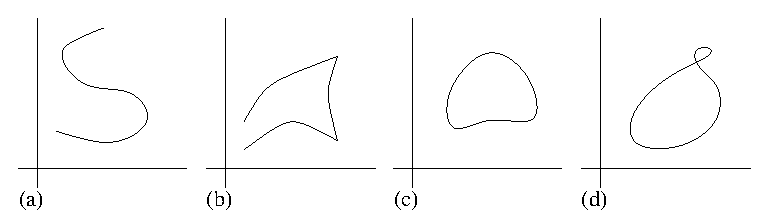
\includegraphics[width=0.8\textwidth]{fcv/function/curves}
  \end{center}
  \caption{(a) Smooth curve. (b) Piecewise smooth curve.
    (c) Simple closed curve. (d) Non-simple closed curve.}
  \label{curves}
\end{figure}






\paragraph{Regions.}
A region $R$ is \textit{connected} if any two points in $R$ can be connected
\index{connected region}
\index{region!connected}
by a curve which lies entirely in $R$.
A region is \textit{simply-connected} if every closed curve
\index{region!simply-connected}
in $R$ can be continuously shrunk to a point without leaving $R$.
A region which is not simply-connected is said to be
\textit{multiply-connected region}.
\index{region!multiply-connected}
Another way of defining simply-connected is that a path connecting two
points in $R$ can be continuously deformed into any other path that connects
those points.  Figure~\ref{regions} shows a simply-connected region with
two paths which can be continuously deformed into one another and two
multiply-connected regions with paths which cannot be deformed into one
another.

\begin{figure}[htb!]
  \begin{center}
      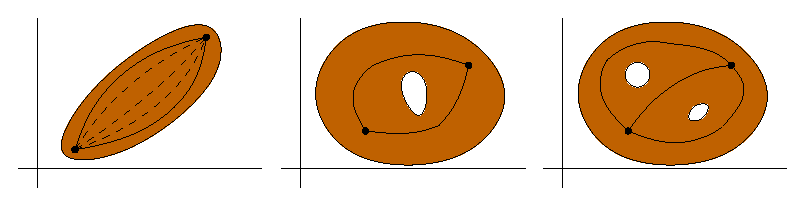
\includegraphics[width=0.9\textwidth]{fcv/function/regions}
  \end{center}
  \caption{A simply-connected and two multiply-connected regions.}
  \label{regions}
\end{figure}





\paragraph{Jordan curve theorem.}
A continuous, simple, closed curve is known as a \textit{Jordan curve}.
\index{curve!Jordan}
\index{Jordan curve}
The Jordan Curve Theorem, which seems intuitively obvious but is difficult
to prove, states that a Jordan curve divides the plane into a simply-connected,
bounded region and an unbounded region.  These two regions are called the
interior and exterior regions, respectively.  The two regions share the
curve as a boundary.  Points in the interior are said to be inside
the curve; points in the exterior are said to be outside the curve.







\paragraph{Traversal of a contour.}
\index{contour!traversal of}
Consider a Jordan curve.  If you traverse the curve in the
\textit{positive} direction, then the inside is to your left.  If you traverse%
\index{direction!positive}
\index{direction!negative}
\index{clockwise}
\index{counter-clockwise}
the curve in the opposite direction, then the outside will be to your
left and you will go around the curve in the negative direction.
For circles, the positive direction is the
\textit{counter-clockwise} direction.   The positive direction is
consistent with the way angles are measured in a right-handed coordinate
system,  i.e. for a circle centered on the origin, the positive direction
is the direction of increasing angle.  For an oriented contour $C$,
we denote the contour with opposite orientation as $-C$.



\paragraph{Boundary of a region.}
Consider a simply-connected region.  The boundary of the region is
traversed in the positive direction if the region is to the left as you
walk along the contour.  For multiply-connected regions, the boundary
may be a set of contours.  In this case the boundary is traversed in the
positive direction if each of the contours is traversed in the positive
direction.  When we refer to the boundary of a region we will assume it
is given the positive orientation.
In Figure~\ref{pos_boundary} the boundaries of three regions
are traversed in the positive direction.

\begin{figure}[htb!]
  \begin{center}
    
\includegraphics[width=0.6\textwidth]{fcv/function/pos_boundary}
  \end{center}
  \caption{Traversing the boundary in the positive direction.}
  \label{pos_boundary}
\end{figure}




\paragraph{Two interpretations of a curve.}
Consider a simple closed curve as depicted in Figure~\ref{two_views}a.
By giving it an orientation, we can make a contour that either
encloses the bounded domain Figure~\ref{two_views}b or the unbounded
domain Figure~\ref{two_views}c.  Thus a curve has two interpretations.
It can be thought of as enclosing either the points which are
``inside'' or the points which are ``outside''.%
\footnote{
  A farmer wanted to know the most efficient way to build a pen to
  enclose his sheep, so he consulted an engineer, a physicist and a
  mathematician.  The engineer suggested that he build a circular pen
  to get the maximum area for any given perimeter.  The physicist
  suggested that he build a fence at infinity and then shrink it to
  fit the sheep.  The mathematician constructed a little fence around
  himself and then defined himself to be outside.
  }


\begin{figure}[htb!]
  \begin{center}
      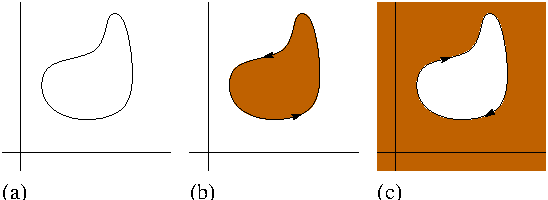
\includegraphics[width=0.6\textwidth]{fcv/function/two_views}
  \end{center}
  \caption{Two interpretations of a curve.}
  \label{two_views}
\end{figure}










%%=============================================================================
\section{The Point at Infinity and the Stereographic Projection}



\paragraph{Complex infinity.}
\index{complex infinity}
\index{infinity!complex}
\index{point at infinity}
\index{infinity!point at}
\index{extended complex plane}
In real variables, there are only two ways to get to infinity.  
We can either go up or down the number line.  Thus signed infinity makes 
sense.  By going up or down we respectively approach $+ \infty$ and $- \infty$.
In the complex plane there are an infinite number of ways to approach 
infinity.  We stand at the origin, point ourselves in any direction and 
go straight.  We could walk along the positive real axis and approach
infinity via positive real numbers.  We could walk along the positive 
imaginary axis and approach infinity via pure imaginary numbers.  We could
generalize the real variable notion of signed infinity to a complex variable
notion of directional infinity, but this will not be useful for our 
purposes.  Instead, we introduce \textit{complex infinity} or
the \textit{point at infinity} as the limit of going infinitely far
along any direction in the complex plane.  The complex plane together with
the point at infinity form the \textit{extended complex plane}.




\paragraph{Stereographic projection.}
\index{stereographic projection}
We can visualize the point at infinity with the 
\textit{stereographic projection}.  We place a unit 
sphere on top of the complex plane so that the south pole of the sphere
is at the origin.  Consider a line passing through the north pole and 
a point $z = x + \imath y$ in the complex plane.  In the stereographic projection,
the point point $z$ is mapped to the point where the line intersects 
the sphere.  (See Figure~\ref{figure stereographic-projection}.)  Each
point $z = x + \imath y$ in the complex plane is mapped to a unique point 
$(X, Y, Z)$ on the sphere.
\[
X = \frac{4 x}{|z|^2 + 4}, \quad
Y = \frac{4 y}{|z|^2 + 4}, \quad
Z = \frac{2 |z|^2}{|z|^2 + 4}
\]
The origin is mapped to the south pole.  The point at infinity, $|z| = \infty$,
is mapped to the north pole.


\begin{figure}[htbp!]
  \begin{center}
      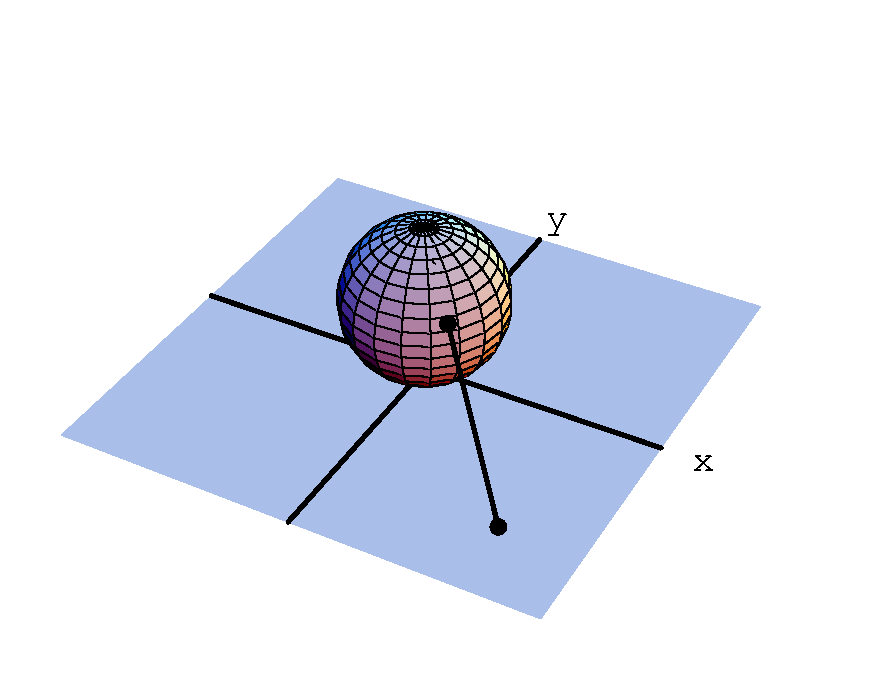
\includegraphics[width=0.5\textwidth]{fcv/function/stereographic-projection}
  \end{center}
  \caption{The stereographic projection.}
  \label{figure stereographic-projection}
\end{figure}



In the stereographic projection, circles in the complex plane are mapped 
to circles on the unit sphere.  Figure~\ref{figure stereo-circle stereo-lines}
shows circles along the real and imaginary axes under the mapping.
Lines in the complex plane are also mapped 
to circles on the unit sphere.  The right diagram in 
Figure~\ref{figure stereo-circle stereo-lines} shows
lines emanating from the origin under the mapping.
\begin{figure}[htbp!]
  \begin{center}
    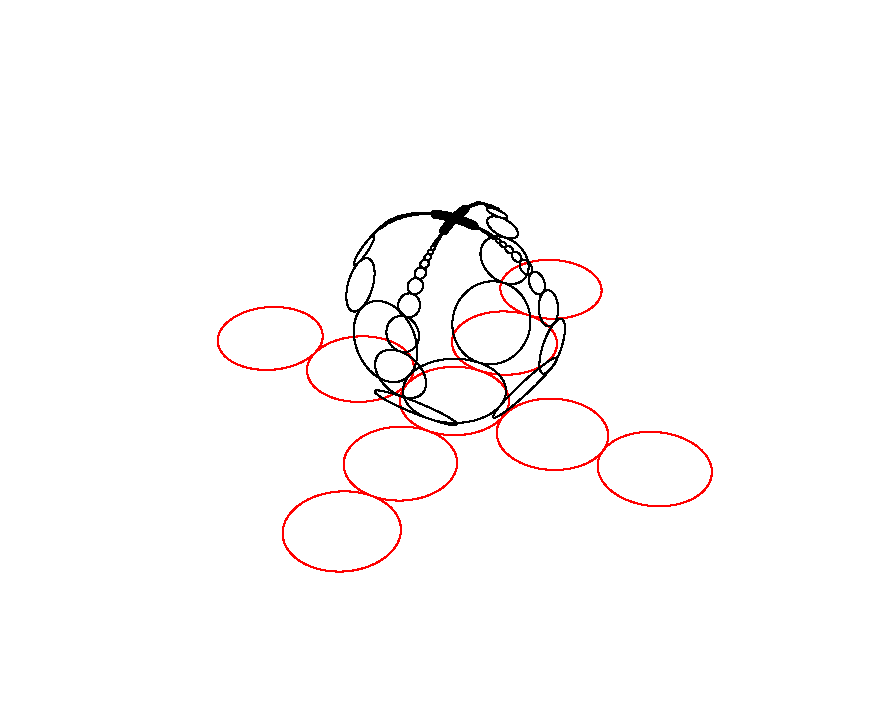
\includegraphics[width=0.49\textwidth]{fcv/function/stereo-circle}
    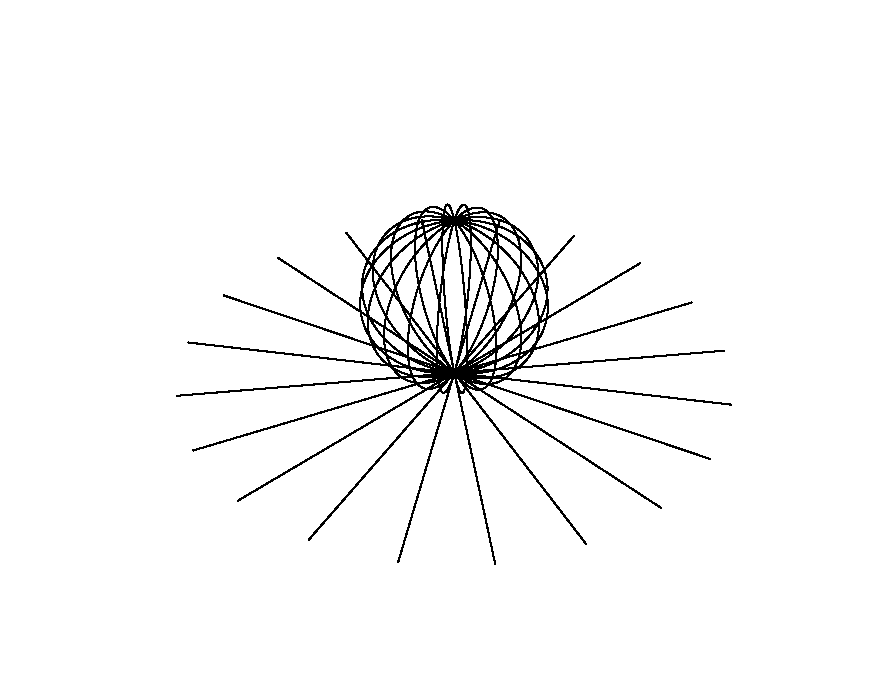
\includegraphics[width=0.49\textwidth]{fcv/function/stereo-line}
  \end{center}
  \caption{The stereographic projection of circles and lines.}
  \label{figure stereo-circle stereo-lines}
\end{figure}


The stereographic projection helps us reason about the point at infinity.
When we consider the complex plane by itself, the point at infinity is an 
abstract notion.  We can't draw a picture of the point at infinity.  It may 
be hard to accept the notion of a jordan curve enclosing the point at 
infinity.  However, in the stereographic projection, the point at infinity
is just an ordinary point (namely the north pole of the sphere).  
%% CONTINUE



%%=============================================================================
\section{A Gentle Introduction to Branch Points}



In this section we will introduce the concepts of \textit{branches}, 
\textit{branch points} and \textit{branch cuts}.  These concepts 
(which are notoriously difficult to understand for beginners)
are typically
defined in terms functions of a complex variable.  Here we will develop
these ideas as they relate to the arctangent function $\arctan(x,y)$.
Hopefully this simple example will make the treatment in 
Section~\ref{chapter function section branch points} more palateable.

First we review some properties of the arctangent.  It is a mapping from
$\mathbb{R}^2$ to $\mathbb{R}$.  It measures the angle around the 
origin from the positive $x$ axis.  Thus it is a multi-valued function.
For a fixed point in the domain, the function values differ by integer 
multiples of $2 \pi$.  The arctangent is not defined at the origin nor 
at the point at infinity; it is singular at these two points.  If we plot 
some of the values of the arctangent, it looks like a corkscrew with 
axis through the origin.  A portion of this function is plotted in
Figure~\ref{arctangent_few}.


\begin{figure}[htbp!]
  \begin{center}
    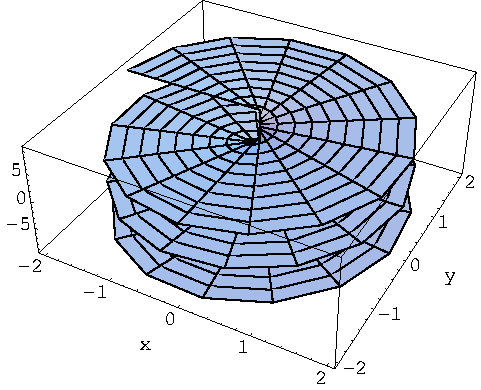
\includegraphics[width=0.4\textwidth]{fcv/function/arctangent_few}
  \end{center}
  \caption{Plots of the real part of the logarithm and a portion of 
    the imaginary part of the logarithm.}
  \label{arctangent_few}
\end{figure}

Most of the tools we have for analyzing functions (continuity, 
differentiability, etc.) depend on the fact that the function is 
single-valued.  In order to work with the arctangent we need to select a 
portion to obtain a single-valued function.  Consider the domain 
$(-1 .. 2) \times (1 .. 4)$.  On this domain we select the value of 
the arctangent that is between $0$ and $\pi$.  The domain and a plot of the 
selected values of the arctangent are shown in 
Figure~\ref{arctangent_square_domain}.

\begin{figure}[htbp!]
  \begin{center}
    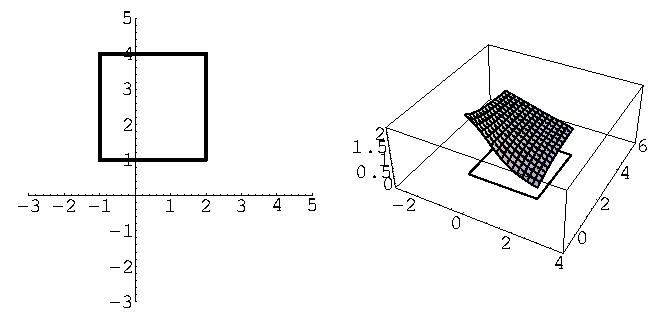
\includegraphics[width=0.7\textwidth]{fcv/function/arctangent_square_domain}
  \end{center}
  \caption{A domain and a selected value of the arctangent for the points
        in the domain.}
  \label{arctangent_square_domain}
\end{figure}




CONTINUE.



%%=============================================================================
\section{Cartesian and Modulus-Argument Form}


We can write a function of a complex variable $z$ as a function of $x$ and $y$
or as a function of $r$ and $\theta$ with the substitutions $z = x + \imath y$
and $z = r \e^{\imath \theta}$, respectively.
Then we can separate the real and imaginary components or write the function
in modulus-argument form,
\[
f(z) = u(x,y) + \imath v(x,y), \quad \mathrm{or} \quad 
f(z) = u(r,\theta) + \imath v(r,\theta),
\]
\[
f(z) = \rho(x,y) \e^{\imath \phi(x,y)}, \quad \mathrm{or} \quad
f(z) = \rho(r,\theta) \e^{\imath \phi(r,\theta)}.
\]



\begin{Example}
  Consider the functions $f(z) = z$, $f(z) = z^3$ and $f(z) = \frac{1}{1-z}$.
  We write the functions in terms of $x$ and $y$ and 
  separate them into their real and imaginary components.
  \begin{align*}
    f(z)    
    &= z 
    \\
    &= x + \imath y
  \end{align*}
  \begin{align*}
    f(z)    
    &= z^3 
    \\
    &= (x + \imath y)^3 
    \\
    &= x^3 + \imath x^2 y - x y^2 - \imath y^3 
    \\
    &= \left( x^3 - x y^2 \right) + \imath \left(x^2 y - y^3 \right)
  \end{align*}
  \begin{align*}
    f(z)    
    &= \frac{1}{1-z} 
    \\
    &= \frac{1}{1 - x - \imath y} 
    \\
    &= \frac{1}{1 - x - \imath y}  \frac{1 - x + \imath y}{1 - x + \imath y} 
    \\
    &= \frac{1-x}{(1-x)^2 + y^2} + \imath \frac{y}{(1-x)^2 + y^2}
  \end{align*}
\end{Example}






\begin{Example}
  Consider the functions $f(z) = z$, $f(z) = z^3$ and $f(z) = \frac{1}{1-z}$.
  We write the functions in terms of $r$ and $\theta$ and 
  write them in modulus-argument form.
  \begin{align*}
    f(z)    
    &= z 
    \\
    &= r \e^{\imath \theta}
  \end{align*}
  \begin{align*}
    f(z)    
    &= z^3 
    \\
    &= \left( r \e^{\imath \theta} \right)^3 
    \\
    &= r^3 \e^{\imath 3 \theta}
  \end{align*}
  \begin{align*}
    f(z)    
    &= \frac{1}{1-z} 
    \\
    &= \frac{1}{1 - r \e^{\imath \theta}} 
    \\
    &= \frac{1}{1 - r \e^{\imath \theta}}  \frac{1}{1 - r \e^{-\imath \theta}} 
    \\
    &= \frac{1 - r \e^{-\imath \theta}}{1 - r \e^{\imath \theta} - r \e^{-\imath \theta} + r^2} 
    \\
    &= \frac{1 - r \cos \theta + \imath r \sin \theta}{1 - 2 r \cos \theta + r^2} 
    \\
    \intertext{Note that the denominator is real and non-negative.}
    &= \frac{1} {1 - 2 r \cos \theta + r^2}  | 1 - r \cos \theta + \imath r \sin \theta | 
    \e^{\imath \arctan(1 - r \cos \theta, r \sin \theta)} 
    \\
    &= \frac{1} {1 - 2 r \cos \theta + r^2}  \sqrt{ (1 - r \cos \theta)^2 + r^2 \sin^2 \theta } 
     \e^{\imath \arctan(1 - r \cos \theta, r \sin \theta)} 
    \\
    &= \frac{1} {1 - 2 r \cos \theta + r^2} 
    \sqrt{ 1 - 2 r \cos \theta + r^2 \cos^2 \theta + r^2 \sin^2 \theta } 
    \e^{\imath \arctan(1 - r \cos \theta, r \sin \theta)} 
    \\
    &= \frac{1}{ \sqrt{ 1 - 2 r \cos \theta + r^2 } }  \e^{\imath \arctan(1 - r \cos \theta, r \sin \theta)} 
  \end{align*}
\end{Example}









%%=============================================================================
\section{Graphing Functions of a Complex Variable}




We cannot directly graph functions of a complex variable as they are 
mappings from $\mathbb{R}^2$ to $\mathbb{R}^2$.  To do so would require four
dimensions.  However, we can can use a surface plot to graph the real part, 
the imaginary part, the modulus or the argument of a function of a complex 
variable.  Each of these are scalar fields, mappings from $\mathbb{R}^2$ to 
$\mathbb{R}$.




\begin{Example}
  Consider the identity function, $f(z) = z$.  In Cartesian coordinates and
  Cartesian form, the function is $f(z) = x + \imath y$.  The real and imaginary
  components are $u(x,y) = x$ and $v(x,y) = y$.  (See Figure~\ref{zreim}.)
  \begin{figure}[htbp!]
    \begin{center}
        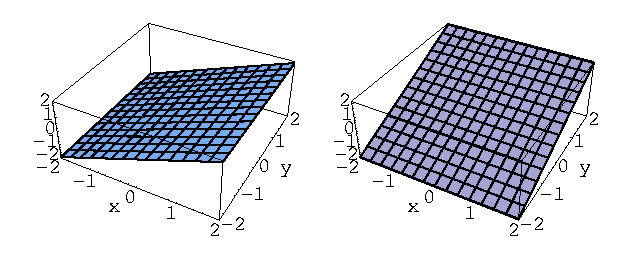
\includegraphics[width=0.6\textwidth]{fcv/function/zreim}
    \end{center}
    \caption{The real and imaginary parts.}
    \label{zreim}
  \end{figure}
  In modulus argument form the function is
  \[
  f(z) = z = r \e^{\imath \theta} = \sqrt{x^2 + y^2}  \e^{\imath \arctan(x,y)}.
  \]
  The modulus of $f(z)$ is a single-valued function which is the distance 
  from the origin.  The argument of $f(z)$ is a multi-valued function.  
  Recall that $\arctan(x,y)$ has an infinite number of values each of
  which differ by an integer multiple of $2 \pi$.  A few branches of 
  $\arg(f(z))$ are plotted in Figure~\ref{zarg}.
  \begin{figure}[htbp!]
    \begin{center}
        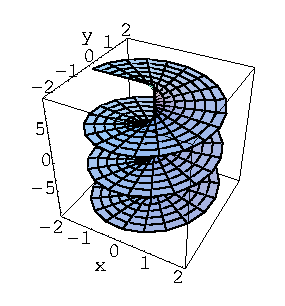
\includegraphics[width=0.25\textwidth]{fcv/function/zarg}
    \end{center}
    \caption{A few branches of the argument function.}
    \label{zarg}
  \end{figure}
  The modulus and principal argument of $f(z) = z$ are plotted in 
  Figure~\ref{zma}.
  \begin{figure}[htbp!]
    \begin{center}
        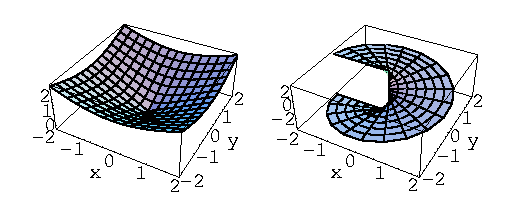
\includegraphics[width=0.5\textwidth]{fcv/function/zma}
    \end{center}
    \caption{Plots of the modulus and argument of \textit{z}.}
    \label{zma}
  \end{figure}
\end{Example}







\begin{Example}
  Consider the function $f(z) = z^2$.  In Cartesian coordinates and separated
  into its real and imaginary components the function is
  \[
  f(z) = z^2 = (x + \imath y)^2 = \left( x^2 - y^2 \right) + \imath 2 x y.
  \]
  Figure~\ref{zsqrreim} shows surface plots of the real and imaginary parts
  of $z^2$.
  \begin{figure}[htbp!]
    \begin{center}
        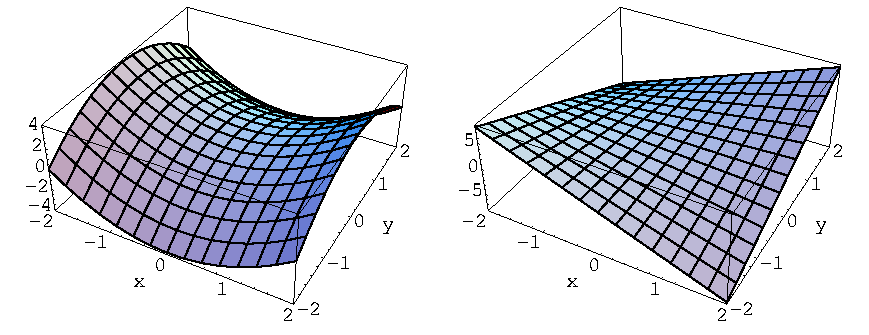
\includegraphics[width=0.8\textwidth]{fcv/function/zsqrreim}
    \end{center}
    \caption{Plots of the real and imaginary parts.}
    \label{zsqrreim}
  \end{figure}
  The magnitude of $z^2$ is
  \[
  |z^2| = \sqrt{z^2 \overline{z^2} } = z \overline{z} 
  = (x + \imath y) (x - \imath y) = x^2 + y^2.
  \]
  Note that 
  \[
  z^2 = \left( r \e^{\imath \theta} \right)^2 = r^2 \e^{\imath 2 \theta}.
  \]
  In Figure~\ref{zsqrma} are plots of $|z^2|$ and a branch of 
  $\arg \left( z^2 \right)$.
  \begin{figure}[htbp!]
    \begin{center}
      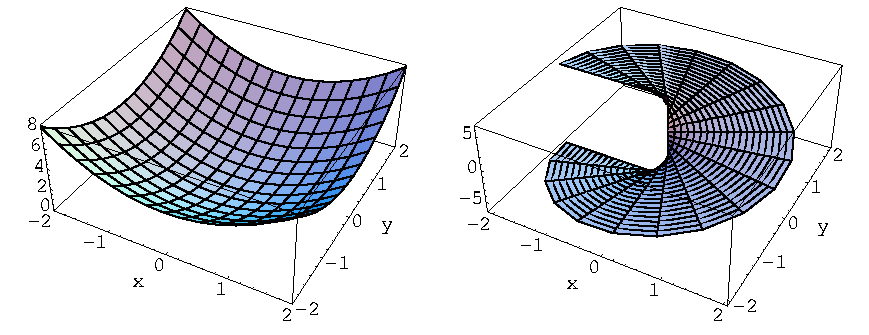
\includegraphics[width=0.8\textwidth]{fcv/function/zsqrma}
    \end{center}
    \caption{Plots of the modulus and a branch of the argument.}
    \label{zsqrma}
  \end{figure}
\end{Example}























%%=============================================================================
\section{Trigonometric Functions}




\paragraph{The exponential function.}
Consider the exponential function $\e^z$.  
We can use Euler's formula to write $\e^z = \e^{x + \imath y}$ in terms of its 
real and imaginary parts. 
\[
\e^z = \e^{x + \imath y} = \e^x \e^{\imath y} = \e^x \cos y + \imath \e^x \sin y
\]
From this we see that the exponential function is $\imath 2 \pi$ periodic:  
$\e^{z + \imath 2 \pi} = \e^z$, and $\imath \pi$ odd periodic: $\e^{z + \imath \pi} = -\e^z$.
Figure~\ref{expreim} has surface plots of the real and imaginary parts
of $\e^z$ which show this periodicity.
\begin{figure}[htbp!]
  \begin{center}
    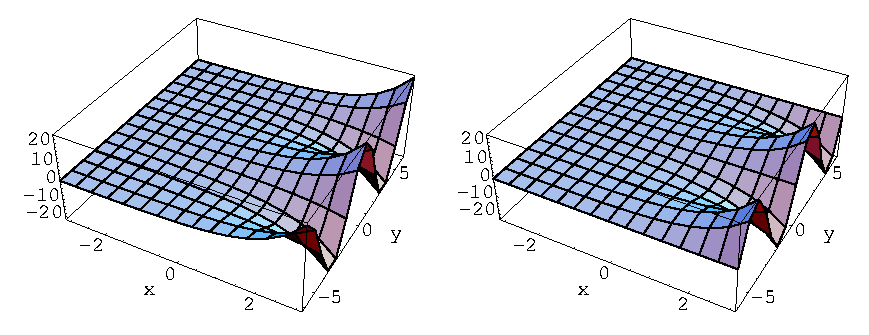
\includegraphics[width=0.8\textwidth]{fcv/function/expreim}
  \end{center}
  \caption{Plots of the real and imaginary parts.}
  \label{expreim}
\end{figure}

The modulus of $\e^z$ is a function of $x$ alone.
\[
\left| \e^z \right| = \left| \e^{x + \imath y} \right| = \e^x
\]
The argument of $\e^z$ is a function of $y$ alone.
\[
\arg \left( \e^z \right) = \arg \left( \e^{x + \imath y} \right) = 
\{ y + 2 \pi n \mid n \in \mathbb{Z} \} 
\]
In Figure~\ref{expma} are plots of $|\e^z|$ and a branch of 
$\arg \left( \e^z \right)$.
\begin{figure}[htbp!]
  \begin{center}
    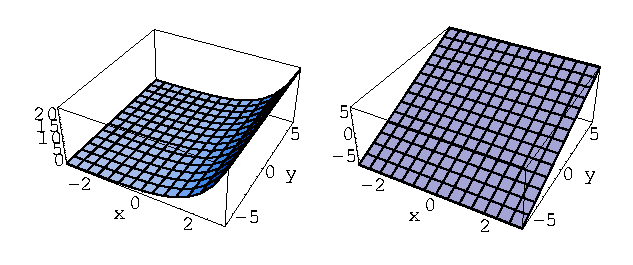
\includegraphics[width=0.6\textwidth]{fcv/function/expma}
  \end{center}
  \caption{Plots of the modulus and a branch of the argument.}
  \label{expma}
\end{figure}







\begin{Example}
  Show that the transformation $w = \e^z$ maps the infinite strip,
  $-\infty < x < \infty$, $0 < y < \pi$, onto the upper half-plane.

  \textbf{Method 1.}
  Consider the line $z = x + \imath c$, $-\infty < x < \infty$.  Under the
  transformation, this is mapped to
  \[ 
  w = \e^{x + \imath c} = \e^{\imath c} \e^x, \quad -\infty < x < \infty. 
  \]
  This is a ray from the origin to infinity in the direction of $\e^{\imath c}$.
  Thus we see that $z = x$ is mapped to the positive, real $w$ axis,
  $z = x + \imath \pi$ is mapped to the negative, real axis, and
  $z = x + \imath c$, $0 < c < \pi$ is mapped to a ray with angle $c$
  in the upper half-plane.  Thus the strip is mapped to the upper half-plane.
  See Figure~\ref{ez_upper_1}.

  \begin{figure}[htbp!]
    \begin{center}
      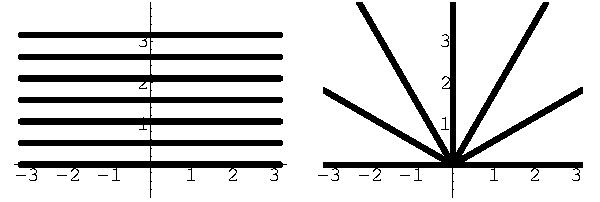
\includegraphics[width=0.6\textwidth]{fcv/function/ez_upper_1}
    \end{center}
    \caption{Horizontal lines are mapped to rays.}
    \label{ez_upper_1}
  \end{figure}

  \textbf{Method 2.}
  Consider the line $z = c + \imath y$, $0 < y < \pi$.  Under the transformation,
  this is mapped to
  \[ 
  w = \e^{c + \imath y} + \e^c \e^{\imath y}, \quad 0 < y < \pi. 
  \]
  This is a semi-circle in the upper half-plane of radius $\e^c$.  As
  $c \to -\infty$, the radius goes to zero.  As $c \to \infty$, the radius
  goes to infinity.  Thus the strip is mapped to the upper half-plane.
  See Figure~\ref{ez_upper_2}.

  \begin{figure}[htbp!]
    \begin{center}
      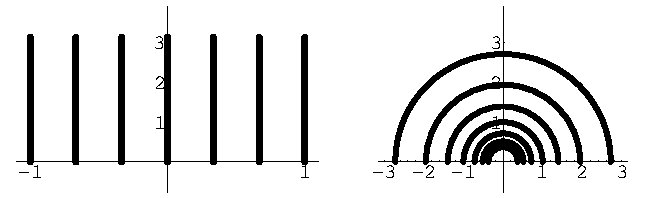
\includegraphics[width=0.6\textwidth]{fcv/function/ez_upper_2}
    \end{center}
    \caption{Vertical lines are mapped to circular arcs.}
    \label{ez_upper_2}
  \end{figure}

\end{Example}









\paragraph{The sine and cosine.}
We can write the sine and cosine in terms of the exponential function.
\begin{align*}
  \frac{ \e^{\imath z} + \e^{-\imath z} }{ 2 }
  &= \frac{ \cos(z) + \imath \sin(z) + \cos(-z) + \imath \sin(-z) }{ 2 } 
  \\
  &= \frac{ \cos(z) + \imath \sin(z) + \cos(z) - \imath \sin(z) }{ 2 } 
  \\
  &= \cos z
\end{align*}
\begin{align*}
  \frac{ \e^{\imath z} - \e^{-\imath z} }{ \imath 2 }
  &= \frac{ \cos(z) + \imath \sin(z) - \cos(-z) - \imath \sin(-z) }{ 2 } 
  \\
  &= \frac{ \cos(z) + \imath \sin(z) - \cos(z) + \imath \sin(z) }{ 2 } 
  \\
  &= \sin z
\end{align*}
We separate the sine and cosine into their real and imaginary parts.
%% CONTINUE cite an exercise.
\[
\cos z = \cos x \cosh y - \imath \sin x \sinh y \qquad
\sin z = \sin x \cosh y + \imath \cos x \sinh y
\]
For fixed $y$, the sine and cosine are oscillatory in $x$.  The amplitude 
of the oscillations grows with increasing $|y|$.  See 
Figure~\ref{cosreim} and Figure~\ref{sinreim} for plots of the real
and imaginary parts of the cosine and sine, respectively.  
Figure~\ref{cosmsinm} shows the modulus of the cosine and the sine.

\begin{figure}[htbp!]
  \begin{center}
    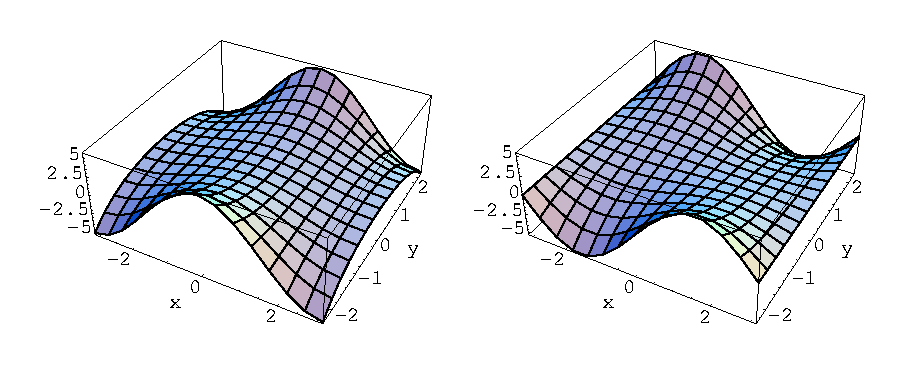
\includegraphics[width=0.8\textwidth]{fcv/function/cosreim}
  \end{center}
  \caption{Plots of the real and imaginary parts of the cosine.}
  \label{cosreim}
\end{figure}

\begin{figure}[htbp!]
  \begin{center}
    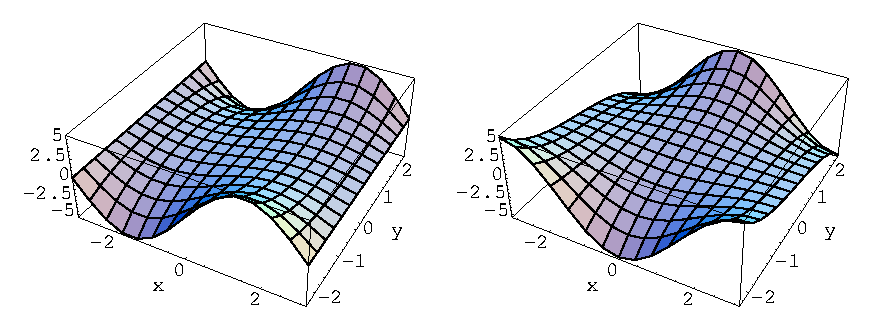
\includegraphics[width=0.8\textwidth]{fcv/function/sinreim}
  \end{center}
  \caption{Plots of the real and imaginary parts of the sine.}
  \label{sinreim}
\end{figure}

\begin{figure}[htbp!]
  \begin{center}
    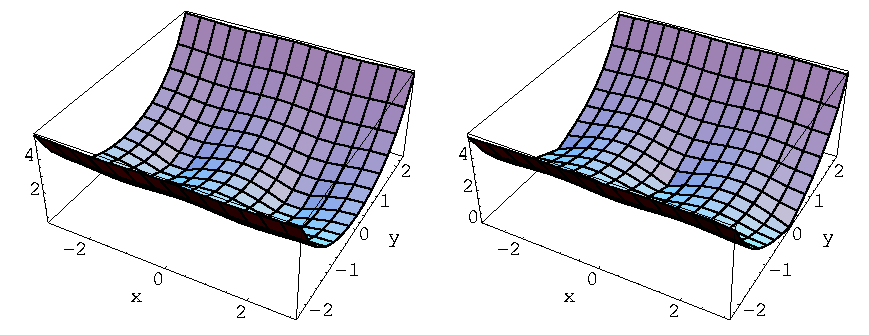
\includegraphics[width=0.8\textwidth]{fcv/function/cosmsinm}
  \end{center}
  \caption{Plots of the modulus of the cosine and the sine.}
  \label{cosmsinm}
\end{figure}



\paragraph{The hyperbolic sine and cosine.}
The hyperbolic sine and cosine have the familiar definitions in terms of the 
exponential function.  Thus not surprisingly, we can write the sine
in terms of the hyperbolic sine and write the cosine in terms of the
hyperbolic cosine.  Below is a collection of trigonometric identities.




\begin{Result}
  \begin{gather*}
    \e^z = \e^x (\cos y + \imath \sin y) 
    \\
    \cos z = \frac{\e^{\imath z} + \e^{-\imath z}}{2} 
    \qquad 
    \sin z = \frac{\e^{\imath z} - \e^{-\imath z}}{\imath 2} 
    \\
    \cos z = \cos x \cosh y - \imath \sin x \sinh y 
    \qquad
    \sin z = \sin x \cosh y + \imath \cos x \sinh y 
    \\
    \cosh z = \frac{\e^z + \e^{-z}}{2} 
    \qquad
    \sinh z = \frac{\e^z - \e^{-z}}{2} 
    \\
    \cosh z = \cosh x \cos y + \imath \sinh x \sin y 
    \qquad
    \sinh z = \sinh x \cos y + \imath \cosh x \sin y 
    \\
    \sin(\imath z) = \imath \sinh z  \qquad \sinh(\imath z) = \imath \sin z 
    \\
    \cos(\imath z) = \cosh z    \qquad \cosh(\imath z) = \cos z 
    \\
    \log z = \ln |z| + \imath \arg(z) 
    = \ln |z| + \imath \Arg(z) + \imath 2 \pi n, \quad n \in \mathbb{Z}
  \end{gather*}
\end{Result}





















%%=============================================================================
\section{Inverse Trigonometric Functions}



\paragraph{The logarithm.}
The logarithm, $\log(z)$, is defined as the inverse of the exponential 
function $\e^z$.  The exponential function is many-to-one and thus 
has a multi-valued inverse.  From what we know of many-to-one functions, we 
conclude that 
\[
\e^{\log z} = z, \quad \mathrm{but} \quad \log \left( \e^z \right) \neq z.
\]
This is because $\e^{\log z}$ is single-valued but $\log \left( \e^z \right)$ is not.
Because $\e^z$ is $\imath 2 \pi$ periodic, the logarithm of a number is 
a set of numbers which differ by integer multiples of $\imath 2 \pi$.  For 
instance, $\e^{\imath 2 \pi n} = 1$ so that 
$\log(1) = \{ \imath 2 \pi n : n \in \mathbb{Z} \}$.
The logarithmic function has an infinite number of branches.  The value of 
the function on the branches differs by integer multiples of $\imath 2 \pi$.  It has 
singularities at zero and infinity.  $|\log(z)| \to \infty$ as either
$z \to 0$ or $z \to \infty$.  

We will derive the formula for the complex variable logarithm.
For now, let $\ln(x)$ denote the real variable logarithm that is defined
for positive real numbers.   Consider $w = \log z$.  This means that
$\e^w = z$.   We write $w = u + \imath v$ in Cartesian form and 
$z = r \e^{\imath \theta}$ in polar form.
\[
\e^{u + \imath v} = r \e^{\imath \theta}
\]
We equate the modulus and argument of this expression.
\begin{gather*}
  \e^u = r \qquad v = \theta + 2 \pi n 
  \\
  u = \ln r \qquad v = \theta + 2 \pi n 
\end{gather*}
With $\log z = u + \imath v$, we have a formula for the logarithm.
\[
\boxed{
  \log z = \ln |z| + \imath \arg(z)
  }
\]
If we write out the multi-valuedness of the argument function we note 
that this has the form that we expected.
\[
\log z = \ln |z| + \imath ( \Arg(z) + 2 \pi n ), \quad n \in \mathbb{Z}
\]
We check that our formula is correct by showing that $\e^{\log z} = z$
\[
\e^{\log z} = \e^{\ln |z| + \imath \arg(z)}
= \e^{\ln r + \imath \theta + \imath 2 \pi n}
= r \e^{\imath \theta}
= z
\]
Note again that $\log \left( \e^z \right) \neq z$.
\[
\log \left( \e^z \right) = \ln |\e^z| + \imath \arg \left( \e^z \right)
= \ln \left( \e^x \right) + \imath \arg \left( \e^{x + \imath y} \right)
= x + \imath (y + 2 \pi n)
= z + \imath 2 n \pi 
\neq z
\]

The real part of the logarithm is the single-valued $\ln r$; 
the imaginary part is the multi-valued $\arg(z)$.
We define the principal branch of the logarithm $\Log z$ to be the branch that 
satisfies $-\pi < \Im(\Log z) \leq \pi$.  For positive, real numbers the
principal branch, $\Log x$ is real-valued.  We can write $\Log z$ in terms of
the principal argument, $\Arg z$.
\[
\Log z = \ln |z| + \imath \Arg(z)
\]
See Figure~\ref{logreim} for plots of the real and imaginary part of 
$\Log z$.

\begin{figure}[htbp!]
  \begin{center}
    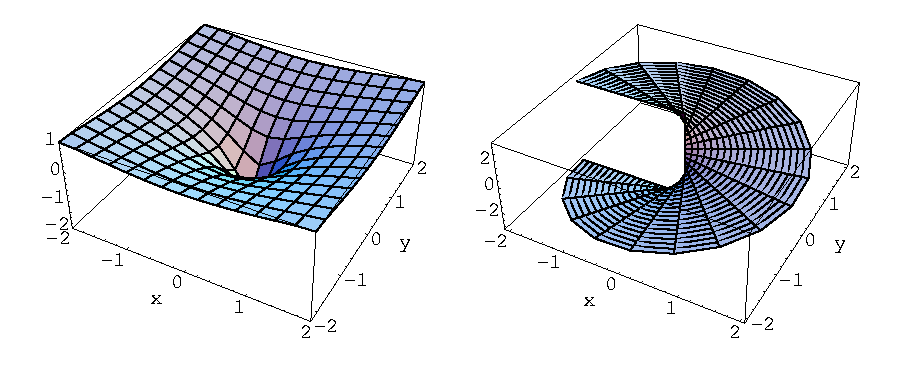
\includegraphics[width=0.8\textwidth]{fcv/function/logreim}
  \end{center}
  \caption{Plots of the real and imaginary parts of the principal branch of
    the logarithm.}
  \label{logreim}
\end{figure}







\paragraph{The form: $\mathbf{a^b}$.}
Consider $a^b$ where $a$ and $b$ are complex and $a$ is nonzero.  We define
this expression in terms of the exponential and the logarithm as
\[
a^b = \e^{b \log a}.
\]
Note that the multi-valuedness of the logarithm may make $a^b$ multi-valued.
First consider the case that the exponent is an integer.
\[
a^m = \e^{m \log a} = \e^{m (\Log a + \imath 2 n \pi)}
= \e^{m \Log a} \e^{\imath 2 m n \pi} = \e^{m \Log a}
\]
Thus we see that $a^m$ has a single value where $m$ is an integer.

Now consider the case that the exponent is a rational number.  Let 
$p/q$ be a rational number in reduced form.
\[
a^{p/q} = \e^{\frac{p}{q} \log a} = \e^{\frac{p}{q}  (\Log a + \imath 2 n \pi)}
= \e^{ \frac{p}{q} \Log a} \e^{\imath 2 n p \pi/q}.
\]
This expression has $q$ distinct values as
\[
\e^{\imath 2 n p \pi / q} = \e^{\imath 2 m p \pi / q} \quad \mathrm{if and only if} \quad
n = m \mod q.
\]

Finally consider the case that the exponent $b$ is an irrational number.
\[
a^b = \e^{b \log a} = \e^{b (\Log a + \imath 2 n \pi) }
= \e^{b \Log a} \e^{\imath 2 b n \pi}
\]
Note that $\e^{\imath 2 b n \pi}$ and
$\e^{\imath 2 b m \pi}$ are equal if and only if $\imath 2 b n \pi$ and $\imath 2 b m \pi$ 
differ by an integer multiple of $\imath 2 \pi$, which means that $b n$ and $b m$ 
differ by an integer.  This occurs only when $n = m$.  Thus $\e^{\imath 2 b n \pi}$
has a distinct value for each different integer $n$.  We conclude that
$a^b$ has an infinite number of values.

You may have noticed something a little fishy.  If $b$ is not an integer
and $a$ is any non-zero complex number, then $a^b$ is multi-valued.
Then why have we been treating $\e^b$ as single-valued, when it is 
merely the case $a = e$?  The answer is that in the realm of functions 
of a complex variable, $\e^z$ is an abuse of notation.  
We write $\e^z$ when we mean $\exp(z)$, the single-valued
exponential function.  Thus when we write $\e^z$ we do not mean 
``the number $e$ raised to the $z$ power'', 
we mean ``the exponential function of $z$''.
We denote the former scenario as $(e)^z$, which is multi-valued.








\paragraph{Logarithmic identities.}
Back in high school trigonometry when you thought that the logarithm was
only defined for positive real numbers you learned the identity
$\log x^a = a \log x$.  This identity doesn't hold when the logarithm is
defined for nonzero complex numbers.  Consider the logarithm of $z^a$.
\[
\log z^a = \Log z^a + \imath 2 \pi n
\]
\[
a \log z = a ( \Log z + \imath 2 \pi n ) = a \Log z + \imath 2 a \pi n
\]
Note that
\[
\log z^a \neq a \log z
\]
Furthermore, since
\[
\Log z^a = \ln |z^a| + \imath \Arg \left( z^a \right), \quad
a \Log z = a \ln |z| + \imath a \Arg(z)
\]
and $\Arg \left( z^a \right)$ is not necessarily the same as $a \Arg(z)$ 
we see that
\[ 
\Log z^a \neq a \Log z. 
\]



Consider the logarithm of a product.
\begin{align*}
  \log(a b) 
  &= \ln |a b| + \imath \arg(a b) 
  \\
  &= \ln |a| + \ln |b| + \imath \arg(a) + \imath \arg(b) 
  \\
  &= \log a + \log b
\end{align*}
There is not an analogous identity for the principal branch of the 
logarithm since $\Arg(a b)$ is not in general the same as 
$\Arg(a) + \Arg(b)$.

Using $\log(a b) = \log(a) + \log(b)$ we can deduce that
$\log \left( a^n \right) = \sum_{k=1}^n \log a = n \log a$, 
where $n$ is a positive integer.
This result is simple, straightforward and wrong.  I have led you down the
merry path to damnation.%
\footnote{
  Don't feel bad if you fell for it.  The logarithm is a 
  tricky bastard.
  }
In fact, $\log \left( a^2 \right) \neq 2 \log a$.  Just write the multi-valuedness
explicitly,
\[
\log \left( a^2 \right) = \Log \left( a^2 \right) + \imath 2 n \pi, \qquad
2 \log a = 2 (\Log a + \imath 2 n \pi) = 2 \Log a + \imath 4 n \pi.
\]


You can verify that 
\[
\log \left( \frac{1}{a} \right) = - \log a.
\]
We can use this and the product identity to expand the logarithm of 
a quotient.
\[
\log \left( \frac{a}{b} \right) = \log a - \log b
\]


For general values of $a$, $\log z^a \neq a \log z$.  However, for some values of 
$a$, equality holds.  We already know that $a = 1$ and $a = -1$ work.  To
determine if equality holds for other values of $a$, we explicitly write the
multi-valuedness.
\begin{gather*}
  \log z^a = \log \left( \e^{a \log z} \right) 
  = a \log z + \imath 2 \pi k, \quad k \in \mathbb{Z} 
  \\
  a \log z = a \ln |z| + \imath a \Arg z + \imath a 2 \pi m, \quad m \in \mathbb{Z}
\end{gather*}
We see that $\log z^a = a \log z$ if and only if
\[
\{ a m \mid m \in \mathbb{Z} \} = \{ a m + k \mid k,m \in \mathbb{Z} \}.
\]
The sets are equal if and only if $a = 1/n$, $n \in \mathbb{Z}^\pm$.  Thus we 
have the identity:
\[
\log \left( z^{1/n} \right) = \frac{1}{n} \log z, \quad n \in \mathbb{Z}^\pm 
\]












\begin{Result}
  \textbf{Logarithmic Identities.}
  \begin{align*}
    &a^b = \e^{b \log a} 
    \\
    &\e^{\log z} = \e^{\Log z} = z 
    \\
    &\log(a b) = \log a + \log b 
    \\
    &\log(1/a) = - \log a 
    \\
    &\log(a/b) = \log a - \log b 
    \\
    &\log \left( z^{1/n} \right) = \frac{1}{n} \log z, \quad n \in \mathbb{Z}^\pm 
  \end{align*}
  \textbf{Logarithmic Inequalities.}
  \begin{align*}
    &\Log(u v) \neq \Log(u) + \Log(v) 
    \\
    &\log z^a \neq a \log z 
    \\
    &\Log z^a \neq a \Log z 
    \\
    &\log \e^z \neq z 
  \end{align*}
\end{Result}









\begin{Example}
  Consider $1^\pi$.  We apply the definition $a^b = \e^{b \log a}$.
  \begin{align*}
    1^\pi    
    &= \e^{\pi \log(1)} 
    \\
    &= \e^{\pi (\ln(1) + \imath 2 n \pi)} 
    \\
    &= \e^{\imath 2 n \pi^2} 
  \end{align*}
  Thus we see that $1^\pi$ has an infinite number of values, all of which
  lie on the unit circle $|z| = 1$ in the complex plane.  However, the set
  $1^\pi$ is not equal to the set $|z| = 1$.  There are points in the 
  latter which are not in the former.  This is analogous to the fact
  that the rational numbers are dense in the real numbers, but are a 
  subset of the real numbers.
\end{Example}







\begin{Example}
  We find the zeros of $\sin z$.

  \begin{gather*}
    \sin z = \frac{\e^{\imath z} - \e^{-\imath z}}{\imath 2} = 0 
    \\
    \e^{\imath z} = \e^{-\imath z} 
    \\
    \e^{\imath 2 z} = 1 
    \\
    2 z \mod 2 \pi = 0 
    \\
    \boxed{ 
      z = n \pi, \quad n \in \mathbb{Z} 
      }
  \end{gather*}

  Equivalently, we could use the identity
  \[ 
  \sin z = \sin x \cosh y + \imath \cos x \sinh y = 0. 
  \]
  This becomes the two equations (for the real and imaginary parts)
  \[ 
  \sin x \cosh y = 0 \qquad \mathrm{and} \qquad \cos x \sinh y = 0. 
  \]
  Since $\cosh$ is real-valued and positive for real argument, 
  the first equation dictates that $x = n \pi$, $n \in \mathbb{Z}$. 
  Since $\cos(n \pi) = (-1)^n$ for $n \in \mathbb{Z}$, the second equation
  implies that $\sinh y = 0$.  For real argument, $\sinh y$ is only zero at
  $y = 0$.  Thus the zeros are
  \[ 
  \boxed{ 
    z = n \pi, \quad n \in \mathbb{Z} 
    } 
  \]
\end{Example}








\begin{Example}
  Since we can express $\sin z$ in terms of the exponential function, one
  would expect that we could express the $\sin^{-1} z$ in terms of the
  logarithm.
  \begin{gather*}
    w =  \sin^{-1} z 
    \\
    z =  \sin w 
    \\
    z =  \frac{\e^{\imath w} - \e^{-\imath w}}{\imath 2} 
    \\
    \e^{\imath 2 w} - \imath 2 z \e^{\imath w} - 1 = 0 
    \\
    \e^{\imath w} =  \imath z \pm \sqrt{1 - z^2} 
    \\
    w =  -\imath \log \left( \imath z \pm \sqrt{1 - z^2} \right)
  \end{gather*}
  Thus we see how the multi-valued $\sin^{-1}$ is related to the logarithm.
  \[
  \boxed{
    \sin^{-1} z =  - \imath \log \left( \imath z \pm \sqrt{1 - z^2} \right)
    }
  \]
\end{Example}











\begin{Example}
  Consider the equation $\sin^3 z = 1$.
  \begin{gather*}
    \sin^3 z = 1 
    \\
    \sin z = 1^{1/3} 
    \\
    \frac{\e^{\imath z} - \e^{-\imath z}}{\imath 2} = 1^{1/3} 
    \\
    \e^{\imath z} - \imath 2 (1)^{1/3} - \e^{-\imath z} = 0 
    \\
    \e^{\imath 2 z} - \imath 2 (1)^{1/3} \e^{\imath z} - 1 = 0 
    \\
    \e^{\imath z} = \frac{\imath 2 (1)^{1/3} \pm \sqrt{-4 (1)^{2/3} + 4}}{2} 
    \\
    \e^{\imath z} = \imath (1)^{1/3} \pm \sqrt{1 - (1)^{2/3}} 
    \\
    \boxed{ 
      z = - \imath \log\left(\imath (1)^{1/3} \pm \sqrt{1 - 1^{2/3}}\right) 
      }
  \end{gather*}
  Note that there are three sources of multi-valuedness in the expression for
  $z$.  The two values of the square root are shown explicitly.  There are
  three cube roots of unity.  Finally, the logarithm has an infinite
  number of branches.  To show this multi-valuedness explicitly, we could write
  \[ 
  \boxed{ 
    z = - \imath \Log\left(\imath \e^{\imath 2 m \pi / 3} \pm \sqrt{1 - \e^{\imath 4 m \pi / 3}}\right)
    + 2 \pi n, \qquad m = 0, 1, 2, \quad n = \ldots, -1, 0, 1, \ldots 
    } 
  \]
\end{Example}









\begin{Example}
  Consider the harmless looking equation, $\imath^z = 1$.

  Before we start with the algebra, note that the right side of the equation
  is a single number.  $\imath^z$ is single-valued only when $z$ is an integer.
  Thus we know that if there are solutions for $z$, they are integers.
  We now proceed to solve the equation.
  \begin{gather*}
    \imath^z = 1 
    \\
    \left( \e^{\imath \pi / 2} \right)^z = 1 
    \\
    \intertext{Use the fact that $z$ is an integer.}
    \e^{\imath \pi z / 2} = 1 
    \\
    \imath \pi z / 2 = \imath 2 n \pi, \quad \mathrm{for some}\ n \in \mathbb{Z} 
    \\
    \boxed{
      z = 4 n, \quad n \in \mathbb{Z}
      }
  \end{gather*}

  Here is a different approach.  We write down the multi-valued form of $\imath^z$.
  We solve the equation by requiring that all the values of $\imath^z$ are $1$.
  \begin{gather*}
    \imath^z = 1 
    \\
    \e^{z \log \imath} = 1 
    \\
    z \log \imath = \imath 2 \pi n, \quad \mathrm{for some}\ n \in \mathbb{Z} 
    \\
    z \left( \imath \frac{\pi}{2} + \imath 2 \pi m \right) = \imath 2 \pi n, \quad \forall 
    m \in \mathbb{Z}, \quad \mathrm{for some}\ n \in \mathbb{Z} 
    \\
    \imath \frac{\pi}{2} z + \imath 2 \pi m z = \imath 2 \pi n, \quad \forall m \in \mathbb{Z},
    \quad \mathrm{for some}\ n \in \mathbb{Z} 
  \end{gather*}
  The only solutions that satisfy the above equation are
  \[
  \boxed{
    z = 4 k, \quad k \in \mathbb{Z}.
    }
  \]

  Now let's consider a slightly different problem: $1 \in \imath^z$.  
  For what values of $z$ does $\imath^z$ have $1$ as one of its values.
  \begin{gather*}
    1 \in \imath^z 
    \\
    1 \in \e^{z \log \imath} 
    \\
    1 \in \{ \e^{z (\imath \pi / 2 + \imath 2 \pi n)} \mid n \in \mathbb{Z} \} 
    \\
    z (\imath \pi / 2 + \imath 2 \pi n) = \imath 2 \pi m, \quad m,n \in \mathbb{Z} 
    \\
    \boxed{
      z = \frac{4 m}{1 + 4 n}, \quad m,n \in \mathbb{Z}
      }
  \end{gather*}
  There are an infinite set of rational numbers for which $\imath^z$ has $1$ as one
  of its values.  For example,
  \[
  \imath^{4/5} = 1^{1/5} =
  \left\{ 1, \e^{\imath 2 \pi / 5}, \e^{\imath 4 \pi / 5}, \e^{\imath 6 \pi / 5}, \e^{\imath 8 \pi / 5} \right\}
  \]
\end{Example}











%%=============================================================================
\section{Riemann Surfaces}

Consider the mapping $w = \log(z)$.  Each nonzero point in the 
$z$-plane is mapped to an infinite number of points in the $w$ plane.
\[
w = \{ \ln |z| + \imath \arg(z) \} 
= \{ \ln |z| + \imath (\Arg(z) + 2 \pi n) \mid n \in \mathbb{Z} \} 
\]
This multi-valuedness makes it hard to work with the logarithm.  We would
like to select one of the branches of the logarithm.  One way of doing 
this is to decompose the $z$-plane into an infinite number of sheets.
The sheets lie above one another and are labeled with the integers, 
$n \in \mathbb{Z}$.  (See Figure~\ref{figure flat-sheets}.)
We label the point $z$ on the $n^{\mathrm{th}}$ sheet as $(z,n)$.  Now each
point $(z,n)$ maps to a single point in the $w$-plane.  For instance,
we can make the zeroth sheet map to the principal branch of the logarithm.
This would give us the following mapping.
\[
\log (z,n) = \Log z + \imath 2 \pi n
\]

\begin{figure}[htbp!]
  \begin{center}
    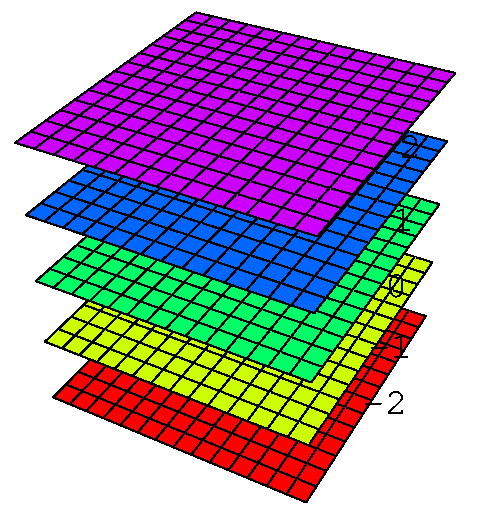
\includegraphics[width=0.3\textwidth]{fcv/function/flat-sheets}
  \end{center}
  \caption{The complex plane decomposed into flat sheets.}
  \label{figure flat-sheets}
\end{figure}



This is a nice idea, but it has some problems.  The mappings are not 
continuous.  Consider the mapping on the zeroth sheet.  As we approach
the negative real axis from above $z$ is mapped to $\ln |z| + \imath \pi$
as we approach from below it is mapped to $\ln |z| - \imath \pi$.
(Recall Figure~\ref{logreim}.)  The mapping is not continuous across the 
negative real axis.

Let's go back to the regular $z$-plane for a moment.
We start at the point $z = 1$ and selecting the branch of the logarithm
that maps to zero.  ($\log(1) = \imath 2 \pi n$).  We make the logarithm
vary continuously as we walk around the origin once in the positive 
direction and return to the point $z = 1$.  Since the argument of $z$
has increased by $2 \pi$, the value of the logarithm has changed to
$\imath 2 \pi$.  If we walk around the origin again we will have 
$\log(1) = \imath 4 \pi$.  Our flat sheet decomposition of the $z$-plane
does not reflect this property.  We need a decomposition with a 
geometry that makes the mapping continuous and connects the various 
branches of the logarithm.


Drawing inspiration from the plot of $\arg(z)$, Figure~\ref{zarg}, we 
decompose the $z$-plane into an infinite corkscrew with axis at the 
origin.  (See Figure~\ref{figure riemann-logz}.)   We define the mapping
so that the logarithm varies continuously on this surface.  
Consider a point $z$ on one of the sheets.  The value of the logarithm 
at that same point on the sheet directly above it is $\imath 2 \pi$ more than 
the original value.  We call this surface, the 
\textit{Riemann surface} for the logarithm.  The mapping from the
Riemann surface to the $w$-plane is continuous and one-to-one.

\begin{figure}[htbp!]
  \begin{center}
    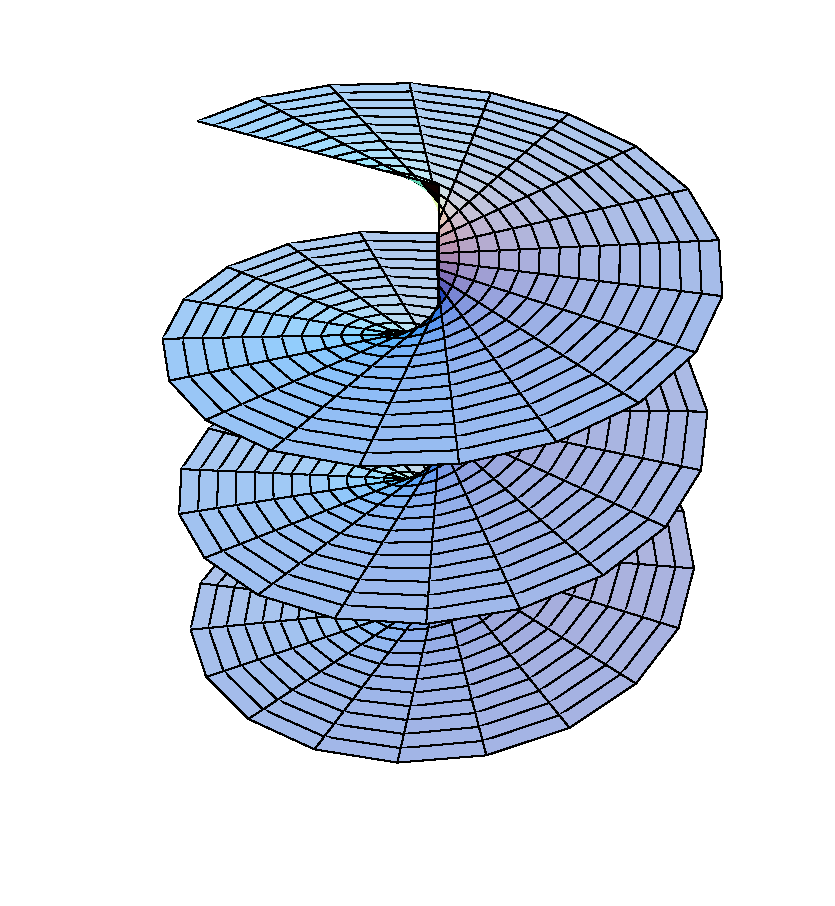
\includegraphics[width=0.3\textwidth]{fcv/function/riemann-logz}
  \end{center}
  \caption{The Riemann surface for the logarithm.}
  \label{figure riemann-logz}
\end{figure}







%%=============================================================================
\section{Branch Points}
\label{chapter function section branch points}
\index{branch point}


%% CONTINUE
%% Before this section:
%% First introduce multi-valuedness in the context of inverse functions of
%% many-to-one mappings.



%% CONTINUE
%% Discover that some multi-valued functions have branch points.






\begin{Example}
  Consider the function $z^{1/2}$.  For each value of $z$, there are
  two values of $z^{1/2}$.  We write $z^{1/2}$ in modulus-argument and 
  Cartesian form.
  \begin{gather*}
    z^{1/2} = \sqrt{|z|} \e^{\imath \arg(z) / 2} 
    \\
    z^{1/2} = \sqrt{|z|} \cos(\arg(z) / 2) + \imath \sqrt{|z|} \sin(\arg(z) / 2)
  \end{gather*}
  Figure~\ref{z_12_re_im} shows the real and imaginary
  parts of $z^{1/2}$ from three different viewpoints.  The second and
  third views are looking down the $x$ axis and $y$ axis,
  respectively.  Consider $\Re \left( z^{1/2} \right)$.  This is a
  double layered sheet which intersects itself on the negative real
  axis.  ($\Im(z^{1/2})$ has a similar structure, but intersects itself
  on the positive real axis.)  Let's start at a point on the positive
  real axis on the lower sheet.  If we walk around the origin once and
  return to the positive real axis, we will be on the upper sheet.  If
  we do this again, we will return to the lower sheet.

  Suppose we are at a point in the complex plane.  We pick one of the
  two values of $z^{1/2}$.  If the function varies continuously as we
  walk around the origin and back to our starting point, the value of
  $z^{1/2}$ will have changed.  We will be on the other branch.
  Because walking around the point $z = 0$ takes us to a different
  branch of the function, we refer to $z = 0$ as a \textit{branch
  point}.

  \begin{figure}[htbp!]
    \begin{center}
      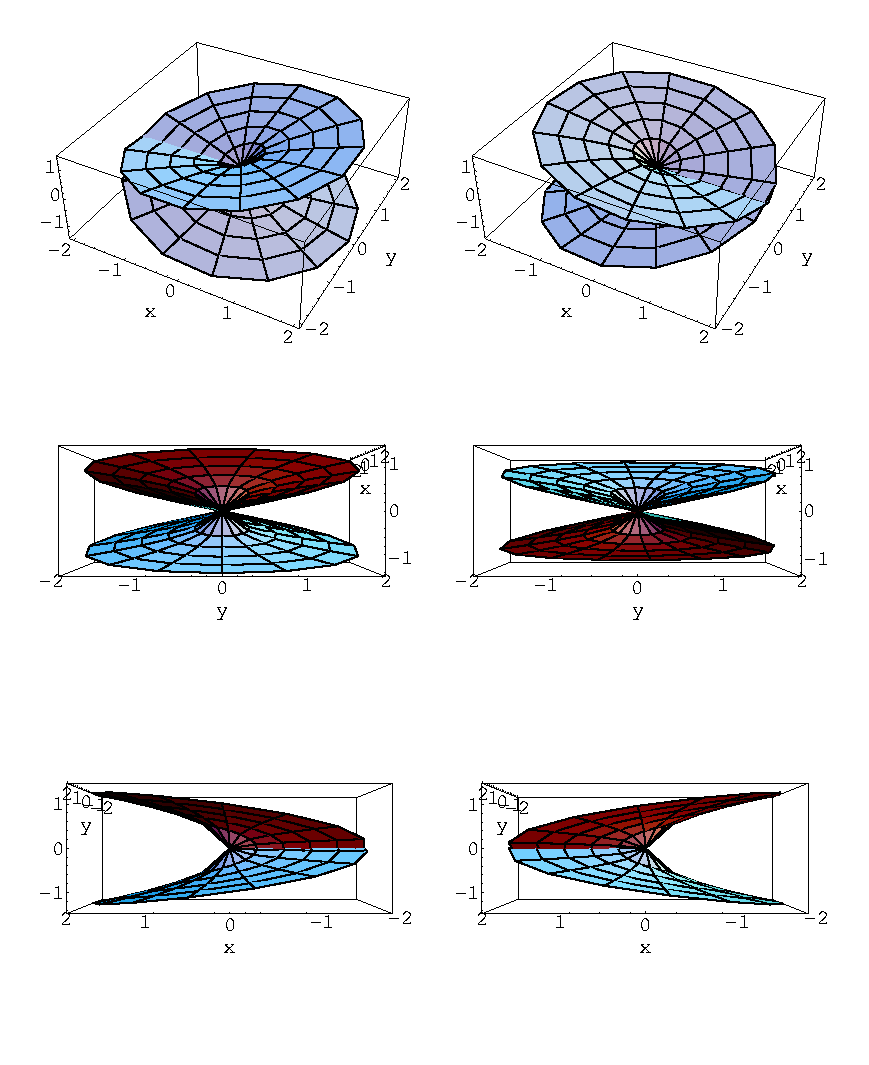
\includegraphics[width=0.55\textwidth]{fcv/function/z_12_re_im}
    \end{center}
    \caption{Plots of the real (left) and 
      imaginary (right) parts from three viewpoints.}
    \label{z_12_re_im}
  \end{figure}

  Now consider the modulus-argument form of $z^{1/2}$:
  \[
  z^{1/2} = \sqrt{|z|} \e^{\imath \arg(z) / 2}.
  \]
  Figure~\ref{z_12_ma} shows the modulus and the principal argument of $z^{1/2}$.
  We see that each time we walk around the origin, the argument of $z^{1/2}$
  changes by $\pi$.  This means that the value of the function changes
  by the factor $\e^{\imath \pi} = -1$, i.e. the function changes sign.  
  If we walk around the origin twice, the argument
  changes by $2 \pi$, so that the value of the function does not change,
  $\e^{\imath 2 \pi} = 1$.

  \begin{figure}[htbp!]
    \begin{center}
      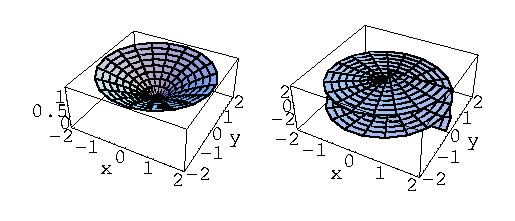
\includegraphics[width=0.5\textwidth]{fcv/function/z_12_ma}
    \end{center}
    \caption{Plots of the modulus and the principal argument.}
    \label{z_12_ma}
  \end{figure}

  $z^{1/2}$ is a continuous function except at
  $z = 0$.  Suppose we start at $z = 1 = \e^{\imath 0}$ and the function value
  $\left( \e^{\imath 0} \right)^{1/2} = 1$.  If we follow the first path in 
  Figure~\ref{unchange_circle_01},
  the argument of $z$
  varies from up to about $\frac{\pi}{4}$, down to about $-\frac{\pi}{4}$
  and back to $0$.  The value of the function is still 
  $\left( \e^{\imath 0} \right)^{1/2}$.

  \begin{figure}[htbp!]
    \begin{center}
      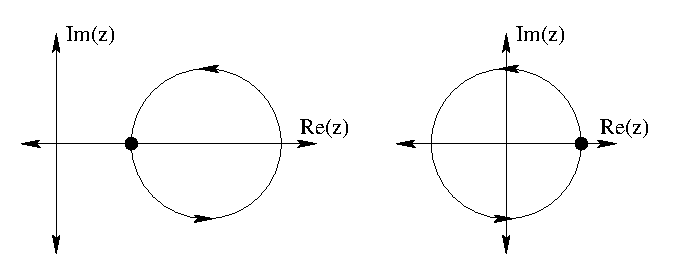
\includegraphics[width=0.5\textwidth]{fcv/function/unchange_change}
    \end{center}
    \caption{A path that does not encircle the origin and a path around 
      the origin.}
    \label{unchange_circle_01}
  \end{figure}

  Now suppose we follow a circular path around the origin in the positive,
  counter-clockwise, direction.  (See the second path in 
  Figure~\ref{unchange_circle_01}.)
  The argument of $z$ increases by $2 \pi$.  The value of the function at
  half turns on the path is
  \begin{align*}
    &\left( \e^{\imath 0} \right)^{1/2} = 1, 
    \\
    &\left( \e^{\imath \pi} \right)^{1/2} = \e^{\imath \pi / 2} = \imath, 
    \\
    &\left( \e^{\imath 2 \pi} \right)^{1/2} = \e^{\imath \pi} = -1
  \end{align*}
  As we return to the point $z = 1$, the argument of the function has changed
  by $\pi$ and the value of the function has changed from $1$ to $-1$.
  If we were to walk along the circular path again, the argument of $z$
  would increase by another $2 \pi$.  The argument of the function would
  increase by another $\pi$ and the value of the function would return to $1$.
  \[
  \left( \e^{\imath 4 \pi} \right)^{1/2} = \e^{\imath 2 \pi} = 1
  \]



  %% CONTINUE: Move this to the next section
  In general, any time we walk around the origin, the value of $z^{1/2}$
  changes by the factor $-1$.  We call $z = 0$ a branch point.  
  If we want a single-valued square root, we need something to prevent us from
  walking around the origin.  We achieve this by introducing a
  branch cut.  Suppose we have the complex plane drawn on an infinite sheet
  of paper. With a scissors we cut the paper from the origin
  to $-\infty$ along the real axis.  Then if we start at $z = \e^{\imath 0}$,
  and draw a continuous line without leaving the paper, the argument of
  $z$ will always be in the range $-\pi < \arg z < \pi$.  This means
  that $-\frac{\pi}{2} < \arg \left( z^{1/2} \right) < \frac{\pi}{2}$.  No matter what
  path we follow in this cut plane, $z = 1$ has argument zero and
  $(1)^{1/2} = 1$.  By never crossing the negative real axis, we have
  constructed a single valued \textbf{branch} of the square root function.
  We call the cut along the negative real axis a \textbf{branch cut}.
\end{Example}






\begin{Example}
  \label{ex_bp_log}
  Consider the logarithmic function $\log z$.  For each value of $z$, there are
  an infinite number of values of $\log z$.  
  We write $\log z$ in Cartesian form.
  \[
    \log z = \ln |z| + \imath \arg z
  \]
  Figure~\ref{logz_reim} shows the real and imaginary parts of the logarithm.
  The real part is single-valued.  The imaginary part is multi-valued and
  has an infinite number of branches.   The values of the logarithm form
  an infinite-layered sheet.  If we start on one of the sheets and walk
  around the origin once in the positive direction, then the value of the
  logarithm increases by $\imath 2 \pi$ and we move to the next branch.
  $z = 0$ is a branch point of the logarithm.

  \begin{figure}[htbp!]
    \begin{center}
      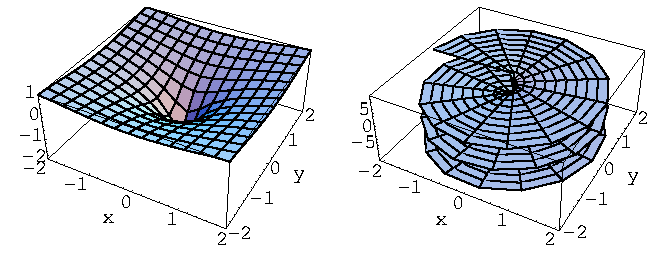
\includegraphics[width=0.6\textwidth]{fcv/function/logz_reim}
    \end{center}
    \caption{Plots of the real part and a portion of imaginary part.}
    \label{logz_reim}
  \end{figure}


  The logarithm is a continuous function except at $z = 0$.  Suppose
  we start at $z = 1 = \e^{\imath 0}$ and the function value $\log\left(
  \e^{\imath 0} \right) = \ln(1) + \imath 0 = 0$.  If we follow the first
  path in Figure~\ref{unchange_circle_01}, the argument of $z$ and
  thus the imaginary part of the logarithm varies from up to about
  $\frac{\pi}{4}$, down to about $-\frac{\pi}{4}$ and back to 0.  The
  value of the logarithm is still $0$.

  Now suppose we follow a circular path around the origin in the positive
  direction.  (See the second path in Figure~\ref{unchange_circle_01}.)
  The argument of $z$ increases by $2 \pi$.  The value of the logarithm at
  half turns on the path is
  \begin{align*}
    &\log\left( \e^{\imath 0} \right) = 0, 
    \\
    &\log\left( \e^{\imath \pi} \right) = \imath \pi, 
    \\
    &\log\left( \e^{\imath 2 \pi} \right) = \imath 2 \pi
  \end{align*}
  As we return to the point $z = 1$, the value of the logarithm has changed
  by $\imath 2 \pi$.
  If we were to walk along the circular path again, the argument of $z$
  would increase by another $2 \pi$ and the value of the logarithm would
  increase by another $\imath 2 \pi$.


  %% CONTINUE: Change to log and Move this to the next section
  %%In general, any time we walk around the origin, the value of $z^{1/2}$
  %%changes by the factor $-1$.  We call $z = 0$ a branch point.  
  %%If we want a single-valued square root, we need something to prevent us from
  %%walking around the origin.  We achieve this by introducing a
  %%branch cut.  Suppose we have the complex plane drawn on an infinite sheet
  %%of paper. With a scissors we cut the paper from the origin
  %%to $-\infty$ along the real axis.  Then if we start at $z = \e^{\imath 0}$,
  %%and draw a continuous line without leaving the paper, the argument of
  %%$z$ will always be in the range $-\pi < \arg z < \pi$.  This means
  %%that $-\frac{\pi}{2} < \arg \left( z^{1/2} \right) < \frac{\pi}{2}$  No matter what
  %%path we follow in this cut plane, $z = 1$ has argument zero and
  %%$(1)^{1/2} = 1$.  By never crossing the negative real axis, we have
  %%constructed a single valued \textbf{branch} of the square root function.
  %%We call the cut along the negative real axis a \textbf{branch cut}.
\end{Example}

















\begin{Result}
  %% CONTINUE
  %% Say this better.
  A point $z_0$ is a \textbf{branch point} of a function $f(z)$ if
  the function changes value when you walk around the point on any
  path that encloses no singularities other than the one at $z = z_0$.
\end{Result}
%% CONTINUE
%% Maybe prove.



\paragraph{Branch points at infinity : mapping infinity to the origin.}
Up to this point we have considered only branch points in the finite
plane.  Now we consider the possibility of a branch point at infinity.
As a first method of approaching this problem we map the point at
infinity to the origin with the transformation $\zeta = 1 / z$ and
examine the point $\zeta = 0$.






\begin{Example}
  Again consider the function $z^{1/2}$.  Mapping the point at infinity to
  the origin, we have $f(\zeta) = (1/\zeta)^{1/2} = \zeta^{-1/2}$.
  For each value of $\zeta$, there are two values of $\zeta^{-1/2}$.  
  We write $\zeta^{-1/2}$ in modulus-argument form.
  \[
  \zeta^{-1/2} = \frac{ 1 }{ \sqrt{|\zeta|} } \e^{- \imath \arg(\zeta) / 2} 
  \]
  Like $z^{1/2}$, $\zeta^{-1/2}$ has a double-layered sheet of values.
  Figure~\ref{zeta_m12_ma} shows the modulus and the principal argument of 
  $\zeta^{-1/2}$.  We see that each time we walk around the origin, the argument
  of $\zeta^{-1/2}$ changes by $-\pi$.  This means that the value of the 
  function changes by the factor $\e^{-\imath \pi} = -1$, i.e. the function changes 
  sign.  If we walk around the origin twice, the argument
  changes by $-2 \pi$, so that the value of the function does not change,
  $\e^{-\imath 2 \pi} = 1$.

  \begin{figure}[htbp!]
    \begin{center}
      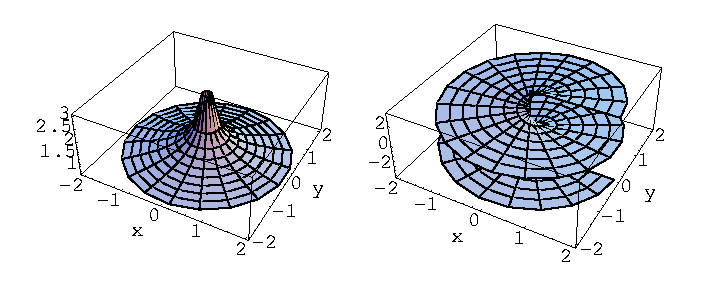
\includegraphics[width=0.6\textwidth]{fcv/function/zeta_m12_ma}
    \end{center}
    \caption{Plots of the modulus and the principal argument.}
    \label{zeta_m12_ma}
  \end{figure}

  Since $\zeta^{-1/2}$ has a branch point at zero, we conclude that $z^{1/2}$
  has a branch point at infinity.
\end{Example}









\begin{Example}
  Again consider the logarithmic function $\log z$.  Mapping the point at 
  infinity to the origin, we have $f(\zeta) = \log(1/\zeta) = - \log(\zeta)$.
  From Example~\ref{ex_bp_log} we known that $- \log(\zeta)$ has a branch
  point at $\zeta = 0$.  Thus $\log z$ has a branch point at infinity.
\end{Example}








\paragraph{Branch points at infinity : paths around infinity.}
We can also check for a branch point at infinity by following a path
that encloses the point at infinity and no other singularities.  
Just draw a simple closed curve that separates the complex plane into
a bounded component that contains all the singularities of the function
in the finite plane.  Then, depending on orientation, the curve is 
a contour enclosing all the finite singularities, or the point at 
infinity and no other singularities.



\begin{Example}
  Once again consider the function $z^{1/2}$.  We know that the function 
  changes value on a curve that goes once around the origin.  Such a 
  curve can be considered to be either a path around the origin or a path
  around infinity.  In either case the path encloses one singularity.  
  There are branch points at the origin and at infinity.  Now consider 
  a curve that does not go around the origin.  Such a curve can be considered
  to be either a path around neither of the branch points or both of them.
  Thus we see that $z^{1/2}$ does not change value when we follow a path
  that encloses neither or both of its branch points.
\end{Example}








\begin{Example}
  Consider $f(z) = \left( z^2 - 1 \right)^{1/2}$.  We factor the function.
  \[
  f(z) = (z - 1)^{1/2}  (z + 1)^{1/2}
  \]
  There are branch points at $z = \pm1$.  Now consider the point at infinity.
  \[
  f\left( \zeta^{-1} \right) = \left( \zeta^{-2} - 1 \right)^{1/2} 
  = \pm \zeta^{-1}  \left( 1 - \zeta^2 \right)^{1/2}
  \]
  Since $f\left( \zeta^{-1} \right)$ does not have a branch point at $\zeta = 0$, $f(z)$
  does not have a branch point at infinity.  We could reach the same
  conclusion by considering a path around infinity.  Consider a path
  that circles the branch points at $z = \pm1$ once in the positive
  direction.  Such a path circles the point at infinity once in the
  negative direction.  In traversing this path, the value of $f(z)$ is
  multiplied by the factor 
  $\left( \e^{\imath 2 \pi} \right)^{1/2}  \left( \e^{\imath 2 \pi} \right)^{1/2} = \e^{\imath 2 \pi} = 1$.  
  Thus the value of the function does not
  change.  There is no branch point at infinity.
\end{Example}







\paragraph{Diagnosing branch points.}
We have the definition of a branch point, but we do not have a convenient
criterion for determining if a particular function has a branch point.
We have seen that $\log z$ and $z^\alpha$ for non-integer $\alpha$ have
branch points at zero and infinity.  The inverse trigonometric functions
like the arcsine also have branch points, but they can be written in terms
of the logarithm and the square root.  In fact all the elementary functions
with branch points can be written in terms of the functions $\log z$ and 
$z^\alpha$.  Furthermore, note that the multi-valuedness of $z^\alpha$
comes from the logarithm,  $z^\alpha = \e^{\alpha \log z}$.
This gives us a way of quickly determining if and where a function
may have branch points.


\begin{Result}
  Let $f(z)$ be a single-valued function.  Then $\log(f(z))$ and 
  $(f(z))^\alpha$ may have branch points only where $f(z)$ is zero or singular.
\end{Result}
%% CONTINUE
%% Prove







\begin{Example}
  Consider the functions,
  \begin{enumerate}
  \item $\left( z^2 \right)^{1/2}$
  \item $\left( z^{1/2} \right)^2$
  \item $\left( z^{1/2} \right)^3$
  \end{enumerate}
  Are they multi-valued?  Do they have branch points?

  \begin{enumerate}
  \item
    \[ 
    \left( z^2 \right)^{1/2} = \pm \sqrt{z^2} = \pm z 
    \]
    Because of the $(\cdot)^{1/2}$, the function is multi-valued.  The
    only possible branch points are at zero and infinity.  If
    $\left( \left( \e^{\imath 0} \right)^2 \right)^{1/2} = 1$, then 
    $\left( \left(\e^{\imath 2 \pi} \right)^2 \right)^{1/2} =
    \left( \e^{\imath 4 \pi} \right)^{1/2} = \e^{\imath 2 \pi} = 1$.  Thus we see that
    the function does not change value when we walk around the origin.
    We can also consider this to be a path around infinity.  This
    function is multi-valued, but has no branch points.
  \item
    \[ 
    \left( z^{1/2} \right)^2 = \left( \pm \sqrt{z} \right)^2 = z 
    \]
    This function is single-valued.
  \item
    \[ 
    \left( z^{1/2} \right)^3 = \left( \pm \sqrt{z} \right)^3 
    = \pm \left( \sqrt{z} \right)^3 
    \]
    This function is multi-valued.  
    We consider the possible branch point at $z = 0$.  If 
    $\left( \left( \e^0 \right)^{1/2} \right)^3 = 1$,
    then $\left( \left( \e^{\imath 2 \pi} \right)^{1/2} \right)^3 = \left( \e^{\imath \pi} \right)^3 
    = \e^{\imath 3 \pi} = -1$.  Since
    the function changes value when we walk around the origin,
    it has a branch point at $z = 0$.  Since this is also a path around 
    infinity, there is a branch point there.
  \end{enumerate}
\end{Example}







\begin{Example}
  Consider the function $f(z) = \log \left( \frac{1}{z-1} \right)$.  Since
  $\frac{1}{z-1}$ is only zero at infinity and its only singularity
  is at $z = 1$, the only possibilities for branch points are at $z = 1$
  and $z = \infty$.  Since
  \[
  \log \left( \frac{1}{z-1} \right) = - \log (z-1)
  \]
  and $\log w$ has branch points at zero and infinity, we see that $f(z)$ 
  has branch points at $z = 1$ and $z = \infty$.
\end{Example}






\begin{Example}
  Consider the functions,
  \begin{enumerate}
  \item $\e^{\log z}$
  \item $\log \e^z$. 
  \end{enumerate}
  Are they multi-valued?  Do they have branch points?

  \begin{enumerate}
  \item
    \[ 
    \e^{\log z} = \exp( \Log z + \imath 2 \pi n ) = \e^{\Log z} \e^{\imath 2 \pi n} = z 
    \]
    This function is single-valued.
  \item
    \[ 
    \log \e^z = \Log \e^z + \imath 2 \pi n = z + \imath 2 \pi m 
    \]
    This function is multi-valued.  It may have branch points only where $\e^z$
    is zero or infinite.  This only occurs at $z = \infty$.
    Thus there are no branch points in the finite plane.  The function does
    not change when traversing a simple closed path.  Since this path can
    be considered to enclose infinity, there is no branch point at infinity.
  \end{enumerate}
\end{Example}






Consider $(f(z))^\alpha$ where $f(z)$ is single-valued and $f(z)$ has either a 
zero or a singularity at $z = z_0$.  $(f(z))^\alpha$ may have a branch point at
$z = z_0$.  If $f(z)$ is not a power of $z$, then it may be difficult to tell
if $(f(z))^\alpha$ changes value when we walk around $z_0$.
Factor $f(z)$ into $f(z) = g(z) h(z)$ where $h(z)$ is nonzero and finite 
at $z_0$.  Then $g(z)$ captures the important behavior of $f(z)$ at the 
$z_0$.  $g(z)$ tells us how fast $f(z)$ vanishes or blows up.  
Since $(f(z))^\alpha = (g(z))^\alpha  (h(z))^\alpha$ and $(h(z))^\alpha$
does not have a branch point at $z_0$, $(f(z))^\alpha$ has a 
branch point at $z_0$ if and only if $(g(z))^\alpha$ has a branch point 
there.

Similarly, we can decompose 
\[
\log(f(z)) = \log(g(z) h(z)) = \log(g(z)) + \log(h(z))
\]
to see that $\log(f(z))$ has a branch point at $z_0$ if and only if
$\log(g(z))$ has a branch point there.





\begin{Result}
  Consider a single-valued function $f(z)$ that has either a zero or
  a singularity at $z = z_0$.  Let $f(z) = g(z) h(z)$ where $h(z)$
  is nonzero and finite.  $(f(z))^\alpha$ has a branch point at $z =
  z_0$ if and only if $(g(z))^\alpha$ has a branch point there.
  $\log(f(z))$ has a branch point at $z = z_0$ if and only if
  $\log(g(z))$ has a branch point there.
\end{Result}








\begin{Example}
  Consider the functions,
  \begin{enumerate}
  \item $\sin z^{1/2}$
  \item $(\sin z)^{1/2}$
  \item $z^{1/2} \sin z^{1/2}$
  \item $\left( \sin z^2 \right)^{1/2}$
  \end{enumerate}
  Find the branch points and the number of branches.

  \begin{enumerate}
    %%
    %%
    %%
  \item
    \[ 
    \sin z^{1/2} = \sin \left( \pm \sqrt{z} \right) = \pm \sin \sqrt{z} 
    \]
    $\sin z^{1/2}$ is multi-valued.  It has two branches.
    There may be branch points at zero and infinity.
    Consider the unit circle which is a path around the origin or infinity.
    If $\sin\left( \left( \e^{\imath 0} \right)^{1/2} \right) = \sin(1)$, then
    $\sin\left( \left( \e^{\imath 2 \pi} \right)^{1/2} \right) = \sin\left( \e^{\imath \pi} \right) 
    = \sin (-1) = - \sin(1)$.
    There are branch points at the origin and infinity.
    %%
    %%
    %%
  \item
    \[ 
    (\sin z)^{1/2} = \pm \sqrt{ \sin z } 
    \]
    The function is multi-valued with two branches.  
    The sine vanishes at $z = n \pi$ and is singular at infinity.  
    There could be branch points at these locations.  
    Consider the point $z = n \pi$.  We can write
    \[
    \sin z = (z - n \pi) \frac{\sin z}{z - n \pi}
    \]
    Note that $\frac{\sin z}{z - n \pi}$ is nonzero and has a
    removable singularity at $z = n \pi$.
    \[
    \lim_{z \to n \pi} \frac{\sin z}{z - n \pi} = \lim_{z \to n \pi} \frac{\cos z}{1} = (-1)^n
    \]
    Since $(z - n \pi)^{1/2}$ has a branch point at $z = n \pi$, $(\sin z)^{1/2}$ has 
    branch points at $z = n \pi$.  

    Since the branch points at $z = n \pi$ go all the way out to infinity.
    It is not possible to make a path that encloses infinity and no other
    singularities.  The point at infinity is a non-isolated singularity.
    A point can be a branch point only if it is an isolated singularity.
    %%
    %%
    %%
  \item 
    \begin{align*}
      z^{1/2} \sin z^{1/2}
      &= \pm \sqrt{z} \sin \left( \pm \sqrt{z} \right) 
      \\
      &= \pm \sqrt{z} \left( \pm \sin \sqrt{z} \right) 
      \\
      &= \sqrt{z} \sin \sqrt{z} 
    \end{align*}
    The function is single-valued.  
    Thus there could be no branch points.
    %%
    %%
    %%
  \item
    \[
    \left( \sin z^2 \right)^{1/2} = \pm \sqrt{ \sin z^2 }
    \]
    This function is multi-valued.  Since $\sin z^2 = 0$ at $z = (n \pi)^{1/2}$,
    there may be branch points there.  First consider the point $z = 0$.
    We can write
    \[
    \sin z^2 = z^2 \frac{\sin z^2}{z^2}
    \]
    where  $\sin\left( z^2 \right) / z^2$ is nonzero and has a removable singularity 
    at $z = 0$.
    \[
    \lim_{z \to 0} \frac{\sin z^2}{z^2} = \lim_{z \to 0} \frac{2 z \cos z^2}{2 z} = 1.
    \]
    Since $\left( z^2 \right)^{1/2}$ does not have a branch point at $z = 0$, 
    $\left( \sin z^2 \right)^{1/2}$
    does not have a branch point there either.

    Now consider the point $z = \sqrt{n \pi}$.
    \[
    \sin z^2 = \left( z - \sqrt{n \pi} \right)  \frac{\sin z^2}{z - \sqrt{n \pi}}
    \]
    $\sin\left( z^2 \right) / \left( z - \sqrt{n \pi} \right)$ in nonzero 
    and has a removable singularity at $z = \sqrt{n \pi}$.
    \[
    \lim_{z \to \sqrt{n \pi}} \frac{\sin z^2}{z - \sqrt{n \pi}}
    = \lim_{z \to \sqrt{n \pi}} \frac{2 z \cos z^2}{1}
    = 2 \sqrt{n \pi} (-1)^n
    \]
    Since $\left( z - \sqrt{n \pi} \right)^{1/2}$ has a branch point at $z = \sqrt{n \pi}$,
    $\left( \sin z^2 \right)^{1/2}$ also has a branch point there.

    Thus we see that $\left( \sin z^2 \right)^{1/2}$ has branch points at 
    $z = (n \pi)^{1/2}$ for $n \in \mathbb{Z} \setminus \{0\}$.
    This is the set of numbers: $\{ \pm \sqrt{\pi}, \pm \sqrt{2 \pi}, \ldots,
    \pm \imath \sqrt{\pi}, \pm \imath \sqrt{2 \pi}, \ldots \}$.
    The point at infinity is a non-isolated singularity.
  \end{enumerate}
\end{Example}









\begin{Example}
  Find the branch points of
  \[ 
  f(z) = \left( z^3 - z \right)^{1/3}. 
  \]
  Introduce branch cuts.  If $f(2) = \sqrt[3]{6}$ then what is $f(-2)$?

  We expand $f(z)$.
  \[ 
  f(z) = z^{1/3} (z-1)^{1/3} (z+1)^{1/3}. 
  \]
  There are branch points at $z = -1, 0, 1$.
  We consider the point at infinity.
  \begin{align*}
    f \left( \frac{1}{\zeta} \right)
    &= \left( \frac{1}{\zeta} \right)^{1/3}  \left( \frac{1}{\zeta}  - 1 \right)^{1/3} 
    \left( \frac{1}{\zeta} + 1 \right)^{1/3} 
    \\
    &= \frac{1}{\zeta}  \left( 1 - \zeta \right)^{1/3}  \left( 1 + \zeta \right)^{1/3}
  \end{align*}
  Since $f(1 / \zeta)$ does not have a branch point at $\zeta = 0$, $f(z)$ does 
  not have a branch point at infinity.
  Consider the three possible branch cuts in Figure~\ref{threebc}.

  \begin{figure}[htb!]
    \begin{center}
      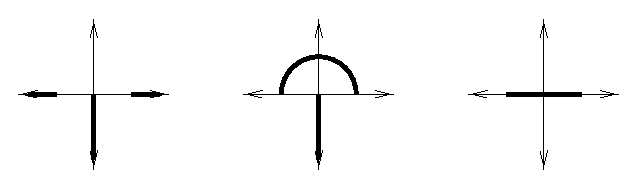
\includegraphics[width=0.7\textwidth]{fcv/function/threebc}
    \end{center}
    \caption{Three possible branch cuts.}
    \label{threebc}
  \end{figure}

  The first and the third branch cuts will make the function single valued,
  the second will not.
  It is clear that the first set makes the function single valued since it
  is not possible to walk around any of the branch points.

  The second set of branch cuts would allow you to walk around the branch
  points at $z = \pm 1$.  If you walked around these two once in the positive
  direction, the value of the function would change by the factor
  $\e^{\imath 4 \pi / 3}$.

  The third set of branch cuts would allow you to walk around all three
  branch points together.  You can verify that if you walk around the
  three branch points, the value of the function will not change
  ($\e^{\imath 6 \pi / 3} = \e^{\imath 2 \pi} = 1$).

  Suppose we introduce the third set of branch cuts and
  are on the branch with $f(2) = \sqrt[3]{6}$.
  \[ 
  f(2) = \left( 2 \e^{\imath 0} \right)^{1/3}  \left( 1 \e^{\imath 0} \right)^{1/3} 
  \left( 3 \e^{\imath 0} \right)^{1/3} = \sqrt[3]{6}
  \]
  The value of $f(-2)$ is
  \begin{align*}
    f(-2)   
    &= \left( 2 \e^{\imath \pi} \right)^{1/3}  \left( 3 \e^{\imath \pi} \right)^{1/3}  
    \left( 1 \e^{\imath \pi} \right)^{1/3} 
    \\
    &= \sqrt[3]{2} \e^{\imath \pi/3} \sqrt[3]{3} \e^{\imath \pi/3} \sqrt[3]{1} \e^{\imath \pi/3} 
    \\
    &= \sqrt[3]{6} \e^{\imath \pi} 
    \\
    &= -\sqrt[3]{6}.
  \end{align*}
\end{Example}






\begin{Example}
  Find the branch points and number of branches for
  \[ 
  f(z) = z^{z^2}. 
  \]

  \[
  z^{z^2} = \exp \left( z^2 \log z \right)
  \]
  There may be branch points at the origin and infinity due to the logarithm.
  Consider walking around a circle of radius $r$ centered at the origin in 
  the positive direction.   Since the logarithm changes by $\imath 2 \pi$, the value
  of $f(z)$ changes by the factor $\e^{\imath 2 \pi r^2}$.  
  There are branch points at the origin and infinity.  The function has an
  infinite number of branches.
\end{Example}









\begin{Example}
  Construct a branch of
  \[ 
  f(z) = \left( z^2 + 1 \right)^{1/3} 
  \]
  such that
  \[ 
  f(0) = \frac{1}{2} \left( -1 + \imath \sqrt{3} \right). 
  \]

  First we factor $f(z)$.
  \[ 
  f(z) = (z - \imath)^{1/3}  (z + \imath)^{1/3}
  \]
  There are branch points at $z = \pm \imath$.  Figure~\ref{singvbc} 
  shows one way to introduce branch cuts.

  \begin{figure}[htb!]
    \begin{center}
      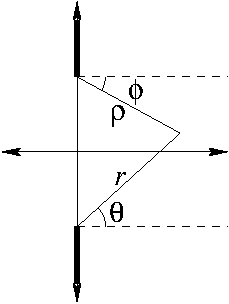
\includegraphics[width=0.2\textwidth]{fcv/function/singvbc}
    \end{center}
    \caption{The branch cuts.}
    \label{singvbc}
  \end{figure}

  Since it is not possible to walk around any branch point, these cuts make
  the function single valued.  We introduce the coordinates:
  \[
  z - \imath = \rho \e^{\imath \phi}, \quad z + \imath = r \e^{\imath \theta}.
  \]
  \begin{align*}
    f(z) &= \left( \rho \e^{\imath \phi} \right)^{1/3}  \left( r \e^{\imath \theta} \right)^{1/3} 
    \\
    &= \sqrt[3]{\rho r} \e^{\imath (\phi+\theta)/3}
  \end{align*}

  The condition
  \[ 
  f(0) = \frac{1}{2} \left( -1 + \imath \sqrt{3} \right) = \e^{\imath (2 \pi/3 + 2 \pi n)} 
  \]
  can be stated
  \begin{gather*}
    \sqrt[3]{1} \e^{\imath (\phi + \theta)/3} = \e^{\imath (2 \pi/3 + 2 \pi n)} 
    \\
    \phi + \theta = 2 \pi + 6 \pi n
  \end{gather*}

  The angles must be defined to satisfy this relation.  One choice is
  \[ 
  \boxed{ 
    \frac{\pi}{2} < \phi < \frac{5 \pi}{2}, \quad
    -\frac{\pi}{2} < \theta < \frac{3 \pi}{2}. 
    } 
  \]
\end{Example}









%% CONTINUE: expand

\paragraph{Principal branches.}
We construct the principal branch of the logarithm by putting a branch
cut on the negative real axis choose $z = r \e^{\imath \theta}$, 
$\theta \in (-\pi,\pi)$.
Thus the principal branch of the logarithm is 
\[
\Log z = \ln r + \imath \theta, \qquad -\pi < \theta < \pi.
\]
Note that the if $x$ is a negative real number, (and thus lies on the 
branch cut), then $\Log x$ is undefined.

The principal branch of $z^\alpha$ is
\[
z^\alpha = \e^{\alpha \Log z}.
\]
Note that there is a branch cut on the negative real axis.
\[
-\alpha \pi < \arg\left( \e^{\alpha \Log z} \right) < \alpha \pi
\]

The principal branch of the $z^{1/2}$ is denoted $\sqrt{z}$.  The 
principal branch of $z^{1/n}$ is denoted $\sqrt[n]{z}$.



\begin{Example}
  Construct $\sqrt{1 - z^2}$, the principal branch of 
  $\left( 1 - z^2 \right)^{1/2}$.

  First note that since $\left( 1 - z^2 \right)^{1/2} = (1 - z)^{1/2}  (1 + z)^{1/2}$ 
  there are branch points at $z = 1$ and $z = -1$.
  The principal branch of the square root has a branch cut on the negative
  real axis.  $1 - z^2$ is a negative real number for $z \in (-\infty \ldots -1)
  \cup (1 \ldots \infty)$.  Thus we put branch cuts on $(-\infty \ldots -1]$ and $[1 \ldots \infty)$.
\end{Example}







\raggedbottom
%%=============================================================================
\exercises{
\pagebreak
\flushbottom
\section{Exercises}




%%-----------------------------------------------------------------------------
\begin{large}
  \noindent
  \textbf{Cartesian and Modulus-Argument Form}
\end{large}





\begin{Exercise}
  \label{exercise image z2}
  Find the image of the strip $2 < x < 3$ under the mapping $w = f(z) = z^2$.
  Does the image constitute a domain?

  \hintsolution{image z2}
\end{Exercise}





%% the transformation $w=z^4$
\begin{Exercise}
  \label{exercise z^4}
  For a given real number $\phi$, $0 \leq \phi < 2 \pi$, find the
  image of the sector $0 \leq \arg(z) < \phi$ under the transformation
  $w = z^4$. How large should $\phi$ be so that the $w$ plane is covered
  exactly once?

  \hintsolution{z^4}
\end{Exercise}




%%-----------------------------------------------------------------------------
\begin{large}
  \noindent
  \textbf{Trigonometric Functions}
\end{large}


%% sin(z) in Cartesian and modulus-argument form
\begin{Exercise}
  \label{exercise sin(z) cart mod-arg}
  In Cartesian coordinates, $z = x + \imath y$, write $\sin(z)$ in Cartesian
  and modulus-argument form.

  \hintsolution{sin(z) cart mod-arg}
\end{Exercise}



%% $\e^z$ is nonzero
\begin{Exercise}
  \label{exercise e z nonzero}
  Show that $\e^z$ is nonzero for all finite $z$.

  \hintsolution{e z nonzero}
\end{Exercise}


%% \left| \e^{z^2} \right| \leq \e^{|z|^2}
\begin{Exercise}
  \label{exercise ez lt ez}
  Show that
  \[
  \left| \e^{z^2} \right| \leq \e^{|z|^2}.
  \]
  When does equality hold?

  \hintsolution{ez lt ez}
\end{Exercise}






%% $\coth z = 1$
\begin{Exercise}
  \label{exercise cothz = 1}
  Solve $\coth(z) = 1$.

  \hintsolution{cothz = 1}
\end{Exercise}



%% 2 \in 2^z
\begin{Exercise}
  \label{exercise 2 in 2z}
  Solve $2 \in 2^z$.  That is, for what values of $z$ is $2$ one of the values
  of $2^z$?  Derive this result then verify your answer by evaluating $2^z$
  for the solutions that your find.

  \hintsolution{2 in 2z}
\end{Exercise}




%% 1 \in 1^z
\begin{Exercise}
  \label{exercise 1 in 1z}
  Solve $1 \in 1^z$.  That is, for what values of $z$ is $1$ one of the values
  of $1^z$?  Derive this result then verify your answer by evaluating $1^z$
  for the solutions that your find.

  \hintsolution{1 in 1z}
\end{Exercise}




%%-----------------------------------------------------------------------------
\begin{large}
  \noindent
  \textbf{Logarithmic Identities}
\end{large}






\begin{Exercise}
  \label{exercise Log z1z2}
  Show that if $\Re \left( z_1 \right) > 0$ and $\Re \left( z_2 \right) > 0$ then
  \[
  \Log( z_1 z_2 ) = \Log( z_1 ) + \Log( z_2 )
  \]
  and illustrate that this relationship does not hold in general.

  \hintsolution{Log z1z2}
\end{Exercise}







%% Find the fallacy in the following argument: \log(-1) = 0.
\begin{Exercise}
  \label{exercise log-1 = 0}
  Find the fallacy in the following arguments:
  \begin{enumerate}
  \item
    $\log(-1) = \log \left( \frac{1}{-1} \right) 
    = \log(1) - \log(-1)
    = - \log(-1)$,
    therefore, $\log(-1) = 0$.
  \item
    $1 = 1^{1/2} = ((-1) (-1))^{1/2} = (-1)^{1/2}  (-1)^{1/2} = \imath \imath =  -1$, 
    therefore, $1 = -1$.
  \end{enumerate}

  \hintsolution{log-1 = 0}
\end{Exercise}











%% modulus-argument and Cartesian form for logarithms
\begin{Exercise}
  \label{exercise mod-arg cart log}
  Write the following expressions in modulus-argument or Cartesian form.
  Denote any multi-valuedness explicitly.
  \[
  2^{2/5}, \quad 3^{1 + \imath}, \quad \left( \sqrt{3} - \imath \right)^{1/4}, \quad 1^{\imath / 4}.
  \]

  \hintsolution{mod-arg cart log}
\end{Exercise}



%% $\cos z = 69$.
\begin{Exercise}
  \label{exercise cosz = 69}
  Solve $\cos z = 69$.

  \hintsolution{cosz = 69}
\end{Exercise}



%% $\cot z = \imath 47$.
\begin{Exercise}
  \label{exercise cotz = i47}
  Solve $\cot z = \imath 47$.

  \hintsolution{cotz = i47}
\end{Exercise}





%% $\log(-\imath)$ $(-\imath)^{-\imath}$ $3^{\pi}$
\begin{Exercise}
  \label{exercise log-i}
  Determine all values of 
  \begin{enumerate}
  \item
    $\log(-\imath)$ 
  \item
    $(-\imath)^{-\imath}$ 
  \item
    $3^{\pi}$
  \item
    $\log(\log(\imath))$
  \end{enumerate}
  and plot them in the complex plane.

  \hintsolution{log-i}
\end{Exercise}





\begin{Exercise}
  \label{exercise cosh ip i2}
Evaluate and plot the following in the complex plane:
\begin{enumerate}
\item 
  $\displaystyle
  ( \cosh(\imath \pi) )^{\imath 2}
  $
\item 
  $\displaystyle
  \log \left( \frac{1}{1 + \imath} \right)
  $
\item 
  $\displaystyle
  \arctan(\imath 3)
  $
\end{enumerate}

  \hintsolution{cosh ip i2}
\end{Exercise}





%% Determine all values of $\imath^\imath$ and $\log((1+\imath)^{\imath \pi})$ and plot them
\begin{Exercise}
  \label{exercise ii log1i}
  Determine all values of $\imath^\imath$ and $\log\left( (1+\imath)^{\imath \pi} \right)$ and 
  plot them in the complex plane.

  \hintsolution{ii log1i}
\end{Exercise}







%% $\e^z = \imath$ $\cos z = \sin z$ $\tan^2 z = -1$
\begin{Exercise}
  Find all $z$ for which
  \begin{enumerate}
  \item
    $\e^z = \imath$ 
  \item
    $\cos z = \sin z$ 
  \item
    $\tan^2 z = -1$
  \end{enumerate}

  \hintsolution{ez = i}
\end{Exercise}






%% \tan^{-1}(z) =\frac{\imath}{2} \log\left( \frac{i+z}{i-z}\right)
\begin{Exercise}
  \label{exercise arctan z}
  Prove the following identities
  and identify the branch points of the functions in the extended 
  complex plane.
  \begin{enumerate}
  \item
    $\displaystyle
    \arctan(z) =\frac{\imath}{2} \log\left( \frac{\imath + z}{\imath - z}\right)
    $
  \item
    $\displaystyle
    \arctanh(z) =\frac{1}{2} \log\left( \frac{1 + z}{1 - z}\right)
    $
  \item
    $\displaystyle
    \arccosh(z) = \log \left( z + \left( z^2 - 1 \right)^{1/2} \right)
    $
  \end{enumerate}

  \hintsolution{arctan z}
\end{Exercise}











%%-----------------------------------------------------------------------------
\begin{large}
  \noindent
  \textbf{Branch Points and Branch Cuts}
\end{large}





\begin{Exercise}
  \label{exercise log zz+1z-1}
  Identify the branch points of the function
  \[
  f(z) = \log \left( \frac{ z (z+1) }{ z-1 } \right)
  \]
  and introduce appropriate branch cuts to ensure that the function is 
  single-valued.

  \hintsolution{log zz+1z-1}
\end{Exercise}





\begin{Exercise}
  \label{exercise z3 z2 6z 12}
  Identify all the branch points of the function
  \[
  w = f(z) = \left( z^3 + z^2 - 6 z \right)^{1/2}
  \]
  in the extended complex plane.  Give a polar description of $f(z)$ and 
  specify branch cuts so that your choice of angles gives a single-valued
  function that is continuous at $z = -1$ with $f(-1) = - \sqrt{6}$.
  Sketch the branch cuts in the stereographic projection.

  \hintsolution{z3 z2 6z 12}
\end{Exercise}








\begin{Exercise}
  \label{exercise mapping z13}
  Consider the mapping $w = f(z) = z^{1/3}$ and the inverse mapping 
  $z = g(w) = w^3$.
  \begin{enumerate}
  \item 
    Describe the multiple-valuedness of $f(z)$.
  \item
    Describe a region of the $w$-plane that $g(w)$ maps one-to-one to the whole
    $z$-plane.
  \item
    Describe and attempt to draw a Riemann surface on which $f(z)$ is 
    single-valued and to which $g(w)$ maps one-to-one.  Comment on the 
    misleading nature of your picture.
  \item
    Identify the branch points of $f(z)$ and introduce a branch cut to make 
    $f(z)$ single-valued.
  \end{enumerate}

  \hintsolution{mapping z13}
\end{Exercise}






%% f(z)=(z^3-1)^{1/2}.
\begin{Exercise}
  \label{exercise z3112}
  Determine the branch points of the function
  \[
  f(z) = \left( z^3 - 1 \right)^{1/2}.
  \]
  Construct cuts and define a branch so that $z = 0$ and $z = -1$ do 
  not lie on a
  cut, and such that $f(0) = -\imath$. What is $f(-1)$ for this branch?

  \hintsolution{z3112}
\end{Exercise}





%% w(z) = \left( (z-1)(z-6)(z+2) \right)^{1/2}
\begin{Exercise}
  \label{exercise z1z6z2}
  Determine the branch points of the function
  \[
  w(z) = \left( (z-1) (z-6) (z+2) \right)^{1/2}
  \]
  Construct cuts and define a branch so that $z = 4$ does not lie
  on a cut, and such that $w = \imath 6$ when $z = 4$.

  \hintsolution{z1z6z2}
\end{Exercise}






%% \cos z^{1/2} (z + \imath)^{-z}
\begin{Exercise}
  \label{exercise cos z12}
  Give the number of branches and locations of the branch points for the 
  functions
  \begin{enumerate}
  \item $\displaystyle \cos \left( z^{1/2} \right)$
  \item $\displaystyle (z + \imath)^{-z}$
  \end{enumerate}

  \hintsolution{cos z12}
\end{Exercise}









%%
\begin{Exercise}
  \label{exercise z2112}
  Find the branch points of the following functions in the extended complex
  plane, (the complex plane including the point at infinity).
  \begin{enumerate}
  \item $\displaystyle \left( z^2 + 1 \right)^{1/2}$
  \item $\displaystyle \left( z^3 - z \right)^{1/2}$
  \item $\displaystyle \log \left( z^2 - 1 \right)$
  \item $\displaystyle \log \left( \frac{z+1}{z-1} \right)$
  \end{enumerate}
  Introduce branch cuts to make the functions single valued.

  \hintsolution{z2112}
\end{Exercise}







%% f(z) = \left( z^3 + 8 \right)^{1/2}
\begin{Exercise}
  \label{exercise z3812}
  Find all branch points and introduce cuts to make the following functions
  single-valued:  For the first function, choose cuts so that there is 
  no cut within the disk $|z| < 2$.
  \begin{enumerate}
  \item $\displaystyle f(z) = \left( z^3 + 8 \right)^{1/2}$
  \item $\displaystyle f(z) 
    = \log \left( 5 + \left( \frac{z+1}{z-1} \right)^{1/2} \right)$
  \item $\displaystyle f(z) = (z + \imath 3)^{1/2}$
  \end{enumerate}

  \hintsolution{z3812}
\end{Exercise}






%% branch point at infinity I
\begin{Exercise}
  \label{exercise bp inf 1}
  Let $f(z)$ have branch points at $z = 0$ and $z = \pm \imath$, but nowhere else
  in the extended complex plane.  How does the value and argument of $f(z)$
  change while traversing the contour in Figure~\ref{cont_around_0pmi}?
  Does the branch cut in Figure~\ref{cont_around_0pmi} make the function 
  single-valued?
  \begin{figure}[htbp!]
    \begin{center}
      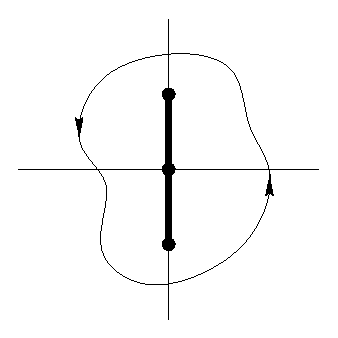
\includegraphics[width=0.25\textwidth]{fcv/function/cont_around_0pmi}
    \end{center}
    \caption{Contour around the branch points and the branch cut.}
    \label{cont_around_0pmi}
  \end{figure}

  \hintsolution{bp inf 1}
\end{Exercise}






%% branch point at infinity II
\begin{Exercise}
  \label{exercise bp inf 2}
  Let $f(z)$ be analytic except for no more than a countably infinite number
  of singularities.  Suppose that $f(z)$ has only one branch point in the
  finite complex plane.  Does $f(z)$ have a branch point at infinity?
  Now suppose that $f(z)$ has two or more branch points in the finite
  complex plane.  Does $f(z)$ have a branch point at infinity?

  \hintsolution{bp inf 2}
\end{Exercise}





%% $(z^4 + 1)^{1/4}
\begin{Exercise}
  \label{exercise z4114}
  Find all branch points of $\left( z^4 + 1 \right)^{1/4}$ in the extended 
  complex plane.
  Which of the branch cuts in Figure~\ref{fourbc} make the function 
  single-valued.
  \begin{figure}[htbp!]
    \begin{center}
      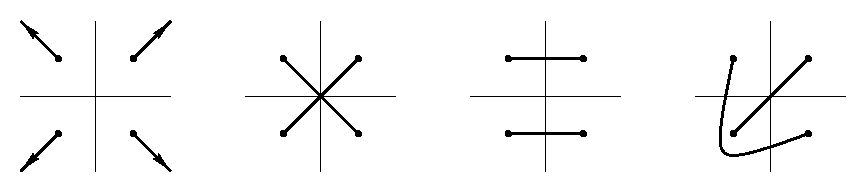
\includegraphics[width=\textwidth]{fcv/function/fourbc}
    \end{center}
    \caption{Four candidate sets of branch cuts.}
    \label{fourbc}
  \end{figure}

  \hintsolution{z4114}
\end{Exercise}






%%
\begin{Exercise}
  \label{exercise zz21}
  Find the branch points of
  \[
  f(z) = \left( \frac{z}{z^2 + 1} \right)^{1/3}
  \]
  in the extended complex plane.  Introduce branch cuts that make the function
  single-valued and such that the function is defined on the positive
  real axis.  Define a branch such that $f(1) = 1 / \sqrt[3]{2}$.  Write
  down an explicit formula for the value of the branch.  What is $f(1 + \imath)$?
  What is the value of $f(z)$ on either side of the branch cuts?

  \hintsolution{zz21}
\end{Exercise}







%% ((z-1)(z-2)(z-3))^{1/2}
\begin{Exercise}
  \label{exercise z1z2z3}
  Find all branch points of 
  \[
  f(z) = ((z-1)(z-2)(z-3))^{1/2}
  \]
  in the extended complex plane.  Which of the branch cuts in
  Figure~\ref{bpbc123} will make the function single-valued.  Using
  the first set of branch cuts in this figure define a branch on which
  $f(0) = \imath \sqrt{6}$.  Write out an explicit formula for the value
  of the function on this branch.
  \begin{figure}[htbp!]
    \begin{center}
      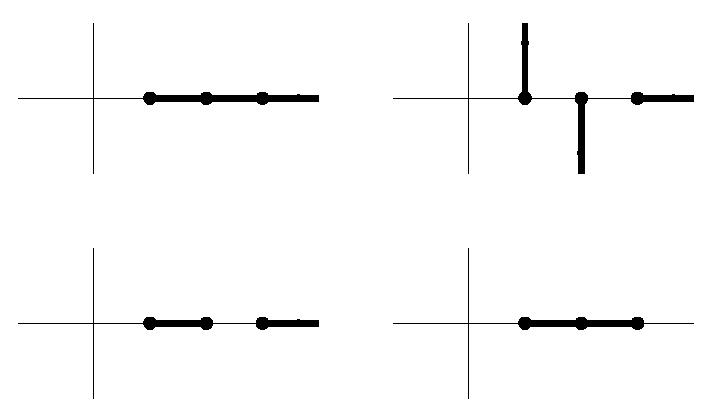
\includegraphics[width=0.5\textwidth]{fcv/function/bpbc123}
    \end{center}
    \caption{Four candidate sets of branch cuts.}
    \label{bpbc123}
  \end{figure}

  \hintsolution{z1z2z3}
\end{Exercise}






%% w = \left( (z^2 - 2)(z + 2) \right)^{1/3}.
\begin{Exercise}
  \label{exercise z22z2}
  Determine the branch points of the function
  \[
  w = \left( \left( z^2 - 2 \right) (z + 2) \right)^{1/3}.
  \]
  Construct and define a branch so that the resulting cut is one line of 
  finite extent and $w(2) = 2$.  What is $w(-3)$ for this branch?  What are 
  the limiting values of $w$ on either side of the branch cut?

  \hintsolution{z22z2}
\end{Exercise}








%%
\begin{Exercise}
  \label{exercise pb arccos}
  Construct the principal branch of $\arccos(z)$.  ($\Arccos(z)$ has the 
  property that if $x \in [-1,1]$ then $\Arccos(x) \in [0,\pi]$.  In 
  particular, $\Arccos(0) = \frac{\pi}{2}$).

  \hintsolution{pb arccos}
\end{Exercise}





%% (z^{1/2} - 1)^{1/2}
\begin{Exercise}
  \label{exercise bp z12112}
  Find the branch points of $\left( z^{1/2} - 1 \right)^{1/2}$ in the finite complex
  plane.  Introduce branch cuts to make the function single-valued.

  \hintsolution{bp z12112}
\end{Exercise}






%% For the linkage illustrated in 
\begin{Exercise}
  \label{exercise linkage}
  For the linkage illustrated in Figure~\ref{linkage}, 
  use complex variables to outline a scheme for 
  expressing the angular position, velocity and acceleration of arm $c$ in
  terms of those of arm $a$.  (You needn't work out the equations.)
  \begin{figure}[htbp!]
    \begin{center}
      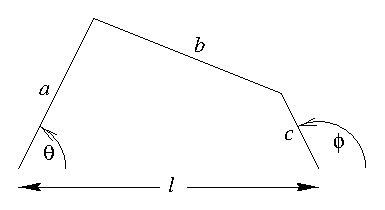
\includegraphics[width=0.4\textwidth]{fcv/function/linkage}
    \end{center}
    \caption{A linkage.}
    \label{linkage}
  \end{figure}

  \hintsolution{linkage}
\end{Exercise}







%% Find the image of the strip $|\Re(z)| < 1$ and of the strip $1 < \Im(z) < 2$
\begin{Exercise}
  \label{exercise image 2z2}
  Find the image of the strip $|\Re(z)| < 1$ and of the strip $1 < \Im(z) < 2$
  under the transformations:
  \begin{enumerate}
  \item
    $w = 2 z^2$
  \item
    $w = \frac{z + 1}{z - 1}$
  \end{enumerate}

  \hintsolution{image 2z2}
\end{Exercise}









%% \frac{(z+1)^{1/2}}{z+2}, \cos \left( \frac{1}{1+z} \right), ...
\begin{Exercise}
  \label{exercise classify z1z2}
  Locate and classify all the singularities of the following functions:
  \begin{enumerate}
  \item $\displaystyle \frac{(z+1)^{1/2}}{z+2}$
  \item $\displaystyle \cos \left( \frac{1}{1+z} \right)$
  \item $\displaystyle \frac{1}{\left( 1 - \e^z \right)^2 }$
  \end{enumerate}
  In each case discuss the possibility of a singularity at the point $\infty$.

  \hintsolution{classify z1z2}
\end{Exercise}








%% Describe how the mapping $w=\sinh(z)$
\begin{Exercise}
  \label{exercise sinh 0 pi}
  Describe how the mapping $w = \sinh(z)$ transforms
  the infinite strip $-\infty < x < \infty$, $0 < y < \pi$ into the
  $w$-plane. Find cuts in the $w$-plane which make the mapping
  continuous both ways. What are the images of the lines (a) $y = \pi / 4$;
  (b) $x = 1$?

  \hintsolution{sinh 0 pi}
\end{Exercise}











\raggedbottom
}
%%=============================================================================
\hints{
\pagebreak
\flushbottom
\section{Hints}





%%-----------------------------------------------------------------------------
\begin{large}
  \noindent
  \textbf{Cartesian and Modulus-Argument Form}
\end{large}





\begin{Hint}
  \label{hint image z2}
  %% CONTINUE
\end{Hint}



%% the transformation $w=z^4$
\begin{Hint}
  \label{hint z^4}
  %% CONTINUE
\end{Hint}



%%-----------------------------------------------------------------------------
\begin{large}
  \noindent
  \textbf{Trigonometric Functions}
\end{large}


%% sin(z) in Cartesian and modulus-argument form
\begin{Hint}
  \label{hint sin(z) cart mod-arg}
  Recall that $\sin(z) = \frac{1}{\imath 2}  \left( \e^{\imath z} - \e^{-\imath z} \right)$.
  Use Result~\ref{cartesian_and_polar_form} to convert between Cartesian
  and modulus-argument form.
\end{Hint}


%% $\e^z$ is nonzero
\begin{Hint}
  \label{hint e z nonzero}
  Write $\e^z$ in polar form.
\end{Hint}




%% \left| \e^{z^2} \right| \leq \e^{|z|^2}
\begin{Hint}
  \label{hint ez lt ez}
  The exponential is an increasing function for real variables.
\end{Hint}







%% $\coth z = 1$
\begin{Hint}
  \label{hint cothz = 1}
  Write the hyperbolic cotangent in terms of exponentials.
\end{Hint}


%% 2 \in 2^z
\begin{Hint}
  \label{hint 2 in 2z}
  Write out the multi-valuedness of $2^z$.  There is a doubly-infinite set of 
  solutions to this problem.
\end{Hint}


%% 1 \in 1^z
\begin{Hint}
  \label{hint 1 in 1z}
  Write out the multi-valuedness of $1^z$.
\end{Hint}





%%-----------------------------------------------------------------------------
\begin{large}
  \noindent
  \textbf{Logarithmic Identities}
\end{large}




\begin{Hint}
  \label{hint Log z1z2}
  %% CONTINUE
\end{Hint}





%% Find the fallacy in the following argument: \log(-1) = 0.
\begin{Hint}
  \label{hint log-1 = 0}
  Write out the multi-valuedness of the expressions.
\end{Hint}





%% modulus-argument and Cartesian form for logarithms
\begin{Hint}
  \label{hint mod-arg cart log}
  Do the exponentiations in polar form.
\end{Hint}



%% $\cos z  = 69$
\begin{Hint}
  \label{hint cosz = 69}
  Write the cosine in terms of exponentials.  Multiply by $\e^{\imath z}$ to get 
  a quadratic equation for $\e^{\imath z}$.
\end{Hint}


%% $\cot z = \imath 47$
\begin{Hint}
  \label{hint cotz = i47}
  Write the cotangent in terms of exponentials.  Get a quadratic equation for
  $\e^{\imath z}$.
\end{Hint}




%% $\log(-\imath)$ $(-\imath)^{-\imath}$ $3^{\pi}$
\begin{Hint}
  \label{hint log-i}
  %% CONTINUE
\end{Hint}





\begin{Hint}
  \label{hint cosh ip i2}
  %% CONTINUE
\end{Hint}




%% Determine all values of $\imath^\imath$ and $\log((1+\imath)^{\imath \pi})$ and plot them
\begin{Hint}
  \label{hint ii log1i}
  $\imath^\imath$ has an infinite number of real, positive values.  $\imath^\imath = \e^{\imath \log \imath}$.
  $\log\left( (1 + \imath)^{\imath \pi} \right)$ has a doubly infinite set of values.
  $\log\left( (1 + \imath)^{\imath \pi} \right) = \log( \exp( \imath \pi \log(1 + \imath) ) )$.
\end{Hint}










%% $\e^z = \imath$ $\cos z = \sin z$ $\tan^2 z = -1$
\begin{Hint}
  \label{hint ez = i}
  %% CONTINUE
\end{Hint}





%% \tan^{-1}(z) =\frac{\imath}{2} \log\left( \frac{i+z}{i-z}\right)
\begin{Hint}
  \label{hint arctan z}
  %% CONTINUE
\end{Hint}



%%-----------------------------------------------------------------------------
\begin{large}
  \noindent
  \textbf{Branch Points and Branch Cuts}
\end{large}


\begin{Hint}
  \label{hint log zz+1z-1}
\end{Hint}





\begin{Hint}
  \label{hint z3 z2 6z 12}
  %% CONTINUE
\end{Hint}






\begin{Hint}
  \label{hint mapping z13}
  %% CONTINUE
\end{Hint}




%% f(z)=(z^3-1)^{1/2}.
\begin{Hint}
  \label{hint z3112}
  %% CONTINUE
\end{Hint}








%% w(z) = \left( (z-1)(z-6)(z+2) \right)^{1/2}
\begin{Hint}
  \label{hint z1z6z2}
  %% CONTINUE
\end{Hint}






%% \cos z^{1/2} (z + \imath)^{-z}
\begin{Hint}
  \label{hint cos z12}
  %% CONTINUE
\end{Hint}






%%
\begin{Hint}
  \label{hint z2112}
  \begin{enumerate}
  \item $\left( z^2 + 1 \right)^{1/2} = (z - \imath)^{1/2}  (z + \imath)^{1/2}$
  \item $\left( z^3 - z \right)^{1/2} = z^{1/2}  (z-1)^{1/2}  (z+1)^{1/2}$
  \item $\log \left( z^2 - 1 \right) = \log (z-1) + \log (z+1)$
  \item $\log \left( \frac{z+1}{z-1} \right) = \log (z+1) - \log (z-1)$
  \end{enumerate}
\end{Hint}










%% f(z) = \left( z^3 + 8 \right)^{1/2}
\begin{Hint}
  \label{hint z3812}
  %% CONTINUE
\end{Hint}







%% branch point at infinity I
\begin{Hint}
  \label{hint bp inf 1}
  Reverse the orientation of the contour so that it encircles infinity and 
  does not contain any branch points.
\end{Hint}




%% branch point at infinity II
\begin{Hint}
  \label{hint bp inf 2}
  Consider a contour that encircles all the branch points in the finite
  complex plane.  Reverse the orientation of the contour so that it 
  contains the point at infinity and does not contain any branch points in
  the finite complex plane.
\end{Hint}




%% $(z^4 + 1)^{1/4}
\begin{Hint}
  \label{hint z4114}
  Factor the polynomial.  The argument of $z^{1/4}$ changes by $\pi / 2$ on 
  a contour that goes around the origin once in the positive direction.
\end{Hint}




%%
\begin{Hint}
  \label{hint zz21}
  %%CONTINUE
\end{Hint}





%% ((z-1)(z-2)(z-3))^{1/2}
\begin{Hint}
  \label{hint z1z2z3}
  To define the branch, define angles from each of the branch points in the
  finite complex plane.
\end{Hint}




%% w = \left( (z^2 - 2)(z + 2) \right)^{1/3}.
\begin{Hint}
  \label{hint z22z2}
  %%CONTINUE
\end{Hint}







%%
\begin{Hint}
  \label{hint pb arccos}
  %%CONTINUE
\end{Hint}






%% (z^{1/2} - 1)^{1/2}
\begin{Hint}
  \label{hint bp z12112}
  %% CONTINUE
\end{Hint}








%% For the linkage illustrated in 
\begin{Hint}
  \label{hint linkage}
  %% CONTINUE
\end{Hint}







%% Find the image of the strip $|\Re(z)| < 1$ and of the strip $1 < \Im(z) < 2$
\begin{Hint}
  \label{hint image 2z2}
  %% CONTINUE
\end{Hint}









%% \frac{(z+1)^{1/2}}{z+2}, \cos \left( \frac{1}{1+z} \right), ...
\begin{Hint}
  \label{hint classify z1z2}
  %% CONTINUE
\end{Hint}




%% Describe how the mapping $w=\sinh(z)$
\begin{Hint}
  \label{hint sinh 0 pi}
  %% CONTINUE
\end{Hint}








\raggedbottom
}
%%=============================================================================
\solutions{
\pagebreak
\flushbottom
\section{Solutions}
}




\solutions{
%%-----------------------------------------------------------------------------
\begin{large}
  \noindent
  \textbf{Cartesian and Modulus-Argument Form}
\end{large}
}




\solutions{
\begin{Solution}
  \label{solution image z2}
  Let $w = u + \imath v$.  We consider the strip $2 < x < 3$ as composed of 
  vertical lines.  Consider the vertical line:
  $z = c + \imath y$, $y \in \mathbb{R}$ for constant $c$.  
  We find the image of this line under the mapping.
  \begin{gather*}
    w = (c + \imath y)^2 
    \\
    w = c^2 - y^2 + \imath 2 c y 
    \\
    u = c^2 - y^2, \quad v = 2 c y 
  \end{gather*}
  This is a parabola that opens to the left.  
  We can parameterize the curve in terms of $v$.
  \[
  u = c^2 - \frac{1}{4 c^2} v^2, \quad v \in \mathbb{R}
  \]
  The boundaries of the region, $x = 2$ and $x = 3$, are respectively 
  mapped to the parabolas:
  \[
  u = 4 - \frac{1}{16} v^2, \quad v \in \mathbb{R}
  \quad \mathrm{and} \quad
  u = 9 - \frac{1}{36} v^2, \quad v \in \mathbb{R}
  \]
  We write the image of the mapping in set notation.
  \[
  \boxed{
    \left\{ w = u + \imath v : v \in \mathbb{R}\ \mathrm{and}\ 
      4 - \frac{1}{16} v^2 < u < 9 - \frac{1}{36} v^2 \right\}.
    }
  \]
  See Figure~\ref{figure domain-image-2x3} for depictions of the strip
  and its image under the mapping.
  The mapping is one-to-one.  Since the image of the strip is open and 
  connected, it is a domain.

  \begin{figure}[htbp!]
    \begin{center}
      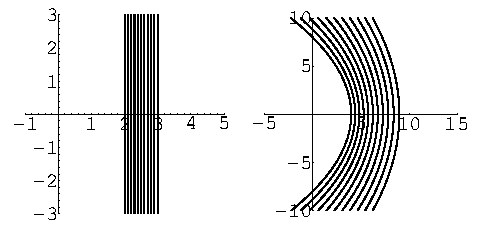
\includegraphics[width=0.5\textwidth]{fcv/function/domain-image-2x3}
    \end{center}
    \caption{The domain and its image under the mapping.}
    \label{figure domain-image-2x3}
  \end{figure}
\end{Solution}
}







%% the transformation $w=z^4$
\solutions{
\begin{Solution}
  \label{solution z^4}
  We write the mapping $w = z^4$ in polar coordinates.
  \[
  w = z^4 = \left( r \e^{\imath \theta} \right)^4 = r^4 \e^{\imath 4 \theta}
  \]
  Thus we see that
  \[
  w : \{ r \e^{\imath \theta} \mid r \geq 0, 0 \leq \theta < \phi \} 
  \to \{ r^4 \e^{\imath 4 \theta} \mid r \geq 0, 0 \leq \theta < \phi \} 
  = \{ r \e^{\imath \theta} \mid r \geq 0, 0 \leq \theta < 4 \phi \} .
  \]
  We can state this in terms of the argument.
  \[
  \boxed{
    w : \{ z \mid 0 \leq \arg(z) < \phi \} 
    \to \{ z \mid 0 \leq \arg(z) < 4 \phi \} 
    }
  \]
  If $\phi = \pi / 2$, the sector will be mapped exactly to the whole complex plane.
\end{Solution}
}





\solutions{
%%-----------------------------------------------------------------------------
\begin{large}
  \noindent
  \textbf{Trigonometric Functions}
\end{large}
}


%% sin(z) in Cartesian and modulus-argument form
\solutions{
\begin{Solution}
  \label{solution sin(z) cart mod-arg}
  \begin{align*}
    \sin z &= \frac{1}{\imath 2} \left( \e^{\imath z} - \e^{-\imath z} \right) 
    \\
    &= \frac{1}{\imath 2} \left( \e^{-y + \imath x} - \e^{y - \imath x} \right) 
    \\
    &= \frac{1}{\imath 2}  \left( \e^{-y} (\cos x + \imath \sin x) 
      - \e^{y}  (\cos x - \imath \sin x) \right) 
    \\
    &= \frac{1}{2}  \left( \e^{-y}  (\sin x - \imath \cos x) 
      + \e^{y}  (\sin x + \imath \cos x) \right) 
    \\
    &= \sin x \cosh y + \imath \cos x \sinh y
  \end{align*}
  \begin{align*}
    \sin z  &= \sqrt{ \sin^2 x \cosh^2 y + \cos^2 x \sinh^2 y } 
    \exp( \imath \arctan( \sin x \cosh y, \cos x \sinh y ) ) 
    \\
    &= \sqrt{ \cosh^2 y - \cos^2 x } 
    \exp( \imath \arctan( \sin x \cosh y, \cos x \sinh y ) ) 
    \\
    &= \sqrt{ \frac{1}{2}  \left( \cosh(2 y) - \cos(2 x) \right) } 
    \exp( \imath \arctan( \sin x \cosh y, \cos x \sinh y ) )
  \end{align*}
\end{Solution}
}


%% $\e^z$ is nonzero
\solutions{
\begin{Solution}
  \label{solution e z nonzero}
  In order that $\e^z$ be zero, the modulus, $\e^x$ must be zero.  Since
  $\e^x$ has no finite solutions, $\e^z = 0$ has no finite solutions.
\end{Solution}
}



%% \left| \e^{z^2} \right| \leq \e^{|z|^2}
\solutions{
\begin{Solution}
  \label{solution ez lt ez}
  We write the expressions in terms of Cartesian coordinates.
  \begin{align*}
    \left| \e^{z^2} \right|
    &= \left| \e^{(x + \imath y)^2} \right| 
    \\
    &= \left| \e^{x^2 - y^2 + \imath 2 x y} \right| 
    \\
    &= \e^{x^2 - y^2}
  \end{align*}
  \[
  \e^{|z|^2}
  = \e^{|x + \imath y|^2} 
  = \e^{x^2 + y^2}
  \]
  The exponential function is an increasing function for real variables.
  Since $x^2 - y^2 \leq x^2 + y^2$, $\e^{x^2 - y^2} \leq \e^{x^2 + y^2}$.
  \[
  \left| \e^{z^2} \right| \leq \e^{|z|^2}
  \]
  Equality holds only when $y = 0$.
\end{Solution}
}




%% $\coth z = 1$
\solutions{
\begin{Solution}
  \label{solution cothz = 1}
  \begin{gather*}
    \coth(z) = 1
    \\
    \frac{ \left( \e^z + \e^{-z} \right) / 2 }{ \left( \e^z - \e^{-z} \right) / 2 } = 1
    \\
    \e^z + \e^{-z} = \e^z - \e^{-z}
    \\
    \e^{-z} = 0
  \end{gather*}
  There are no solutions.
\end{Solution}
}



%% 2 \in 2^z
\solutions{
\begin{Solution}
  \label{solution 2 in 2z}
  We write out the multi-valuedness of $2^z$.
  \begin{gather*}
    2 \in 2^z 
    \\
    \e^{\ln 2} \in \e^{z \log(2)} 
    \\
    \e^{\ln 2} \in \{ \e^{z (\ln(2) + \imath 2 \pi n)} \mid n \in \mathbb{Z} \} 
    \\
    \ln 2 \in z \{ \ln 2 + \imath 2 \pi n + \imath 2 \pi m \mid m,n \in \mathbb{Z} \} 
    \\
    \boxed{
      z = \left\{ \frac{ \ln(2) + \imath 2 \pi m }{ \ln(2) + \imath 2 \pi n } \mid 
        m,n \in \mathbb{Z} \right\}
      }
  \end{gather*}
  We verify this solution.  Consider $m$ and $n$ to be fixed integers.
  We express the multi-valuedness in terms of $k$.
  \begin{align*}
    2^{(\ln(2) + \imath 2 \pi m)/(\ln(2) + \imath 2 \pi n)}
    &= \e^{(\ln(2) + \imath 2 \pi m)/(\ln(2) + \imath 2 \pi n) \log (2)} 
    \\
    &= \e^{(\ln(2) + \imath 2 \pi m)/(\ln(2) + \imath 2 \pi n) 
      (\ln (2) + \imath 2 \pi k)}
  \end{align*}
  For $k = n$, this has the value, $\e^{\ln(2) + \imath 2 \pi m} = \e^{\ln(2)} = 2$.
\end{Solution}
}




%% 1 \in 1^z
\solutions{
\begin{Solution}
  \label{solution 1 in 1z}
  We write out the multi-valuedness of $1^z$.
  \begin{gather*}
    1 \in 1^z 
    \\
    1 \in \e^{z \log(1)} 
    \\
    1 \in \{ \e^{\imath z 2 \pi n} \mid n \in \mathbb{Z} \}
  \end{gather*}
  The element corresponding to $n = 0$ is $\e^0 = 1$.
  Thus $1 \in 1^z$ has the solutions,
  \[
  \boxed{
    z \in \mathbb{C}.
    }
  \]
  That is, $z$ may be any complex number.  We verify this solution.
  \[
  1^z = \e^{z \log(1)} = \e^{\imath z 2 \pi n}
  \]
  For $n = 0$, this has the value $1$.
\end{Solution}
}





\solutions{
%%-----------------------------------------------------------------------------
\begin{large}
  \noindent
  \textbf{Logarithmic Identities}
\end{large}
}





\solutions{
\begin{Solution}
  \label{solution Log z1z2}
  We write the relationship in terms of the natural logarithm and the 
  principal argument.
  \begin{gather*}
    \Log( z_1 z_2 ) = \Log( z_1 ) + \Log( z_2 )
    \\
    \ln| z_1 z_2 | + \imath \Arg( z_1 z_2 ) 
    = \ln| z_1 | + \imath \Arg( z_1 ) + \ln| z_2 | + \imath \Arg( z_2 ) 
    \\
    \Arg( z_1 z_2 ) = \Arg( z_1 ) + \Arg( z_2 ) 
  \end{gather*}
  $\Re \left( z_k \right) > 0$ implies that $\Arg( z_k ) \in (-\pi/2 \ldots \pi/2)$.  Thus
  $\Arg( z_1 ) + \Arg( z_2 ) \in (-\pi \ldots \pi)$. In this case the relationship holds.

  The relationship does not hold in general because $\Arg( z_1 ) + \Arg( z_2 )$
  is not necessarily in the interval $(-\pi \ldots \pi]$.  Consider $z_1 = z_2 = -1$.
  \begin{gather*}
    \Arg((-1) (-1)) = \Arg(1) = 0, \qquad
    \Arg( -1 ) + \Arg( -1 ) = 2 \pi
    \\
    \Log((-1) (-1)) = \Log(1) = 0, \qquad
    \Log( -1 ) + \Log( -1 ) = \imath 2 \pi
  \end{gather*}
\end{Solution}
}







%% Find the fallacy in the following argument: \log(-1) = 0.
\solutions{
\begin{Solution}
  \label{solution log-1 = 0}
  \begin{enumerate}
    %%
    %%
    %%
  \item
    The algebraic manipulations are fine.  We write out the multi-valuedness 
    of the logarithms.
    \[
    \log(-1) = \log \left( \frac{1}{-1} \right) 
    = \log(1) - \log(-1)
    = - \log(-1) 
    \]
    \begin{multline*}
      \{ \imath \pi + \imath 2 \pi n: n \in \mathbb{Z} \} 
      = \{ \imath \pi + \imath 2 \pi n: n \in \mathbb{Z} \} 
      \\
      = \{ \imath 2 \pi n: n \in \mathbb{Z} \} 
      - \{ \imath \pi + \imath 2 \pi n: n \in \mathbb{Z} \} 
      = \{ - \imath \pi - \imath 2 \pi n: n \in \mathbb{Z} \} 
    \end{multline*}
    Thus $\log(-1) = - \log(-1)$.  However
    this does not imply that $\log(-1) = 0$.  This is because the logarithm
    is a set-valued function $\log(-1) = - \log(-1)$ is really saying:
    \[
    \{ \imath \pi + \imath 2 \pi n: n \in \mathbb{Z} \} 
    = \{ - \imath \pi - \imath 2 \pi n: n \in \mathbb{Z} \} 
    \]
    %%
    %%
    %%
  \item
    We consider
    \[
    1 = 1^{1/2} = ((-1) (-1))^{1/2} = (-1)^{1/2}  (-1)^{1/2} = \imath \imath =  -1.
    \]
    There are three multi-valued expressions above.
    \begin{gather*}
      1^{1/2} = \pm 1 
      \\
      ((-1) (-1))^{1/2} = \pm 1 
      \\
      (-1)^{1/2}  (-1)^{1/2} = (\pm \imath) (\pm \imath) = \pm 1
    \end{gather*}
    Thus we see that the first and fourth equalities are incorrect.
    \[
    1 \neq 1^{1/2}, \quad  (-1)^{1/2}  (-1)^{1/2} \neq \imath \imath
    \]
  \end{enumerate}
\end{Solution}
}






%% modulus-argument and Cartesian form for logarithms
\solutions{
\begin{Solution}
  \label{solution mod-arg cart log}
  \begin{align*}
    2^{2/5}
    &= 4^{1/5} 
    \\
    &= \sqrt[5]{4}  1^{1/5} 
    \\
    &= \sqrt[5]{4} \e^{\imath 2 n \pi/5}, \quad n = 0,1,2,3,4
  \end{align*}

  \begin{align*}
    3^{1+\imath}
    &= \e^{(1 + \imath) \log 3} 
    \\
    &= \e^{(1 + \imath) (\ln 3 + \imath 2 \pi n)} 
    \\
    &= \e^{\ln 3 - 2 \pi n} \e^{ \imath (\ln 3 + 2 \pi n)}, \quad  n \in \mathbb{Z}
  \end{align*}

  \begin{align*}
    \left( \sqrt{3} - \imath \right)^{1/4}
    &= \left( 2 \e^{-\imath \pi / 6} \right)^{1/4} 
    \\
    &= \sqrt[4]{2} \e^{-\imath \pi / 24} 1^{1/4} 
    \\
    &= \sqrt[4]{2} \e^{\imath (\pi n / 2 - \pi / 24)}, \quad n = 0,1,2,3
  \end{align*}

  \begin{align*}
    1^{\imath / 4}
    &= \e^{(\imath / 4) \log 1} 
    \\
    &= \e^{(\imath / 4) (\imath 2 \pi n)} 
    \\
    &= \e^{- \pi n/2}, \quad n \in \mathbb{Z}
  \end{align*}
\end{Solution}
}



%% $\cos z = 69$
\solutions{
\begin{Solution}
  \label{solution cosz = 69}
  \begin{gather*}
    \cos z = 69 \\
    \frac{\e^{\imath z} + \e^{-\imath z}}{2} = 69 
    \\
    \e^{\imath 2 z} - 138 \e^{\imath z} + 1 = 0 
    \\
    \e^{\imath z} = \frac{1}{2} \left( 138 \pm \sqrt{138^2 - 4} \right) 
    \\
    z = -\imath \log \left( 69 \pm 2 \sqrt{1190} \right) 
    \\
    z = -\imath \left( \ln \left( 69 \pm 2 \sqrt{1190} \right) 
      + \imath 2 \pi n \right) 
    \\
    \boxed{
      z = 2 \pi n - \imath \ln \left( 69 \pm 2 \sqrt{1190} \right), \quad
      n \in \mathbb{Z}
      }
  \end{gather*}
\end{Solution}
}




%% $\cot z = \imath 47$
\solutions{
\begin{Solution}
  \label{solution cotz = i47}
  \begin{gather*}
    \cot z = \imath 47 
    \\
    \frac{\left(\e^{\imath z} + \e^{-\imath z} \right)/2}
    {\left( \e^{\imath z} - \e^{-\imath z} \right)/(\imath 2)} = \imath 47 
    \\
    \e^{\imath z} + \e^{-\imath z} = 47 \left( \e^{\imath z} - \e^{-\imath z} \right) 
    \\
    46 \e^{\imath 2 z} - 48 = 0 
    \\
    \imath 2 z = \log \frac{24}{23} 
    \\
    z = - \frac{\imath}{2} \log \frac{24}{23} 
    \\
    z = - \frac{\imath}{2} \left( \ln \frac{24}{23} + \imath 2 \pi n \right), \quad
    n \in \mathbb{Z} 
    \\
    \boxed{
      z =  \pi n - \frac{\imath}{2} \ln \frac{24}{23}, \quad n \in \mathbb{Z} 
      }
  \end{gather*}
\end{Solution}
}







%% $\log(-\imath)$ $(-\imath)^{-\imath}$ $3^{\pi}$
\solutions{
\begin{Solution}
  \label{solution log-i}
  \begin{enumerate}
    %%
    %%
    %%
  \item
    \begin{align*}
      \log(-\imath)
      &= \ln |-\imath| + \imath \arg(-\imath) 
      \\
      &= \ln(1) + \imath \left( - \frac{\pi}{2} + 2 \pi n \right), 
      \quad n \in \mathbb{Z} 
    \end{align*}
    \[
    \boxed{
      \log(-\imath) = - \imath \frac{\pi}{2} + \imath 2 \pi n, \quad n \in \mathbb{Z} 
      }
    \]
    These are equally spaced points in the imaginary axis.  See 
    Figure~\ref{log_mi}.

    \begin{figure}[htbp!]
      \begin{center}
        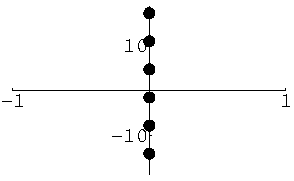
\includegraphics[width=0.3\textwidth]{fcv/function/log_mi}
      \end{center}
      \caption{Plot of the values.}
      \label{log_mi}
    \end{figure}
    %%
    %%
    %%
  \item
    \begin{align*}
      (-\imath)^{-\imath}
      &= \e^{-\imath \log(-\imath)} 
      \\
      &= \e^{-\imath (-\imath \pi/2 + \imath 2 \pi n)}, \quad n \in \mathbb{Z}
    \end{align*}
    \[
    \boxed{
      (-\imath)^{-\imath} = \e^{-\pi/2 + 2 \pi n}, \quad n \in \mathbb{Z} 
      }
    \]
    These are points on the positive real axis with an accumulation point 
    at the origin.  See Figure~\ref{mi_mi}.

    \begin{figure}[htbp!]
      \begin{center}
        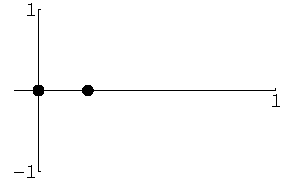
\includegraphics[width=0.3\textwidth]{fcv/function/mi_mi}
      \end{center}
      \caption{Plot of the values.}
      \label{mi_mi}
    \end{figure}
    %%
    %%
    %%
  \item
    \begin{align*}
      3^\pi
      &= \e^{\pi \log(3)} 
      \\
      &= \e^{\pi (\ln(3) + \imath \arg(3))} 
    \end{align*}
    \[
    \boxed{
      3^\pi = \e^{\pi (\ln(3) + \imath 2 \pi n)}, \quad n \in \mathbb{Z} 
      }
    \]
    These points all lie on the circle of radius $|e^\pi|$ centered about
    the origin in the complex plane.  See Figure~\ref{3_pi}.

    \begin{figure}[htbp!]
      \begin{center}
        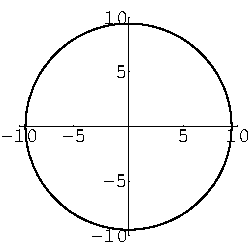
\includegraphics[width=0.25\textwidth]{fcv/function/3_pi}
      \end{center}
      \caption{Plot of the values.}
      \label{3_pi}
    \end{figure}
    %%
    %%
    %%
  \item
    \begin{align*}
      \log(\log(\imath))
      &= \log \left( \imath \left( \frac{\pi}{2} + 2 \pi m \right) \right), 
      \quad m \in \mathbb{Z} 
      \\
      &= \ln \left| \frac{\pi}{2} + 2 \pi m \right|
      + \imath \Arg \left( \imath \left( \frac{\pi}{2} + 2 \pi m \right) \right)
      + \imath 2 \pi n,
      \quad m,n \in \mathbb{Z} 
      \\
      &= \ln \left| \frac{\pi}{2} + 2 \pi m \right|
      + \imath \sign(1 + 4 m) \frac{\pi}{2} + \imath 2 \pi n,
      \quad m,n \in \mathbb{Z} 
    \end{align*}
    These points all lie in the right half-plane.
    See Figure~\ref{loglogi}.

    \begin{figure}[htbp!]
      \begin{center}
        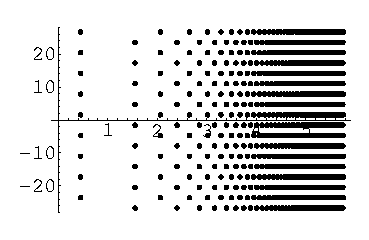
\includegraphics[width=0.4\textwidth]{fcv/function/loglogi}
      \end{center}
      \caption{Plot of the values.}
      \label{loglogi}
    \end{figure}
  \end{enumerate}
\end{Solution}
}






\solutions{
\begin{Solution}
  \label{solution cosh ip i2}
\begin{enumerate}
\item 
  \begin{align*}
    ( \cosh(\imath \pi) )^{\imath 2}
    &= \left( \frac{ \e^{\imath \pi} + \e^{-\imath \pi} }{2} \right)^{\imath 2}
    \\
    &= (-1)^{\imath 2}
    \\
    &= \e^{\imath 2 \log(-1)}
    \\
    &= \e^{\imath 2 (\ln(1) + \imath \pi + \imath 2 \pi n)}, \quad n \in \mathbb{Z}
    \\
    &= \e^{- 2 \pi (1 + 2 n)}, \quad n \in \mathbb{Z}
  \end{align*}
  These are points on the positive real axis with an accumulation point 
  at the origin.  See Figure~\ref{figure coshipi2}.
  \begin{figure}[htbp!]
    \begin{center}
      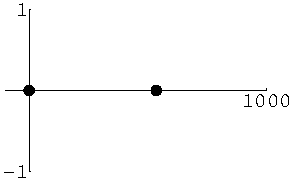
\includegraphics[width=0.3\textwidth]{fcv/function/coshipi2}
    \end{center}
    \caption{Plot of the values.}
    \label{figure coshipi2}
  \end{figure}
\item 
  \begin{align*}
    \log \left( \frac{1}{1 + \imath} \right)
    &= - \log ( 1 + \imath )
    \\
    &= - \log \left( \sqrt{2} \e^{\imath \pi/4} \right)
    \\
    &= - \frac{1}{2} \ln(2) - \log \left( \e^{\imath \pi/4} \right)
    \\
    &= - \frac{1}{2} \ln(2) - \imath \pi/4 + \imath 2 \pi n, \quad n \in \mathbb{Z}
  \end{align*}
  These are points on a vertical line in the complex plane.
  See Figure~\ref{figure log11i}.
  \begin{figure}[htbp!]
    \begin{center}
      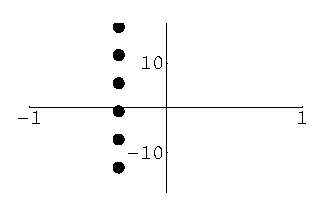
\includegraphics[width=0.3\textwidth]{fcv/function/log11i}
    \end{center}
    \caption{Plot of the values.}
    \label{figure log11i}
  \end{figure}
\item 
  \begin{align*}
    \arctan(\imath 3)
    &= \frac{1}{\imath 2} \log \left( \frac{ \imath - \imath 3 }{ \imath + \imath 3 } \right)
    \\
    &= \frac{1}{\imath 2} \log \left( - \frac{1}{2} \right)
    \\
    &= \frac{1}{\imath 2} \left( \ln \left( \frac{1}{2} \right) 
      + \imath \pi + \imath 2 \pi n \right), \quad n \in \mathbb{Z}
    \\
    &= \frac{\pi}{2} + \pi n + \frac{\imath}{2} \ln(2)
  \end{align*}
  These are points on a horizontal line in the complex plane.
  See Figure~\ref{figure arctani3}.
  \begin{figure}[htbp!]
    \begin{center}
      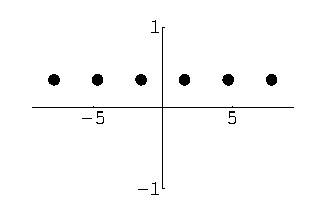
\includegraphics[width=0.3\textwidth]{fcv/function/arctani3}
    \end{center}
    \caption{Plot of the values.}
    \label{figure arctani3}
  \end{figure}
\end{enumerate}
\end{Solution}
}









%% Determine all values of $\imath^\imath$ and $\log((1+\imath)^{\imath \pi})$ and plot them
\solutions{
\begin{Solution}
  \label{solution ii log1i}
  \begin{align*}
    \imath^\imath     
    &= \e^{\imath \log(\imath)} 
    \\
    &= \e^{\imath (\ln|\imath| + \imath \Arg(\imath) + \imath 2 \pi n) }, \quad n \in \mathbb{Z} 
    \\
    &= \e^{\imath ( \imath \pi / 2 + \imath 2 \pi n) }, \quad n \in \mathbb{Z} 
    \\
    &= \e^{-\pi ( 1/2 + 2 n) }, \quad n \in \mathbb{Z} 
  \end{align*}
  These are points on the positive real axis.  There is an accumulation point 
  at $z = 0$.  See Figure~\ref{i_i}.

  \begin{figure}[htbp!]
    \begin{center}
      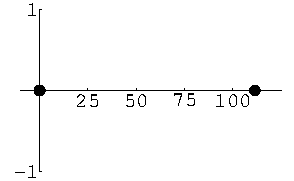
\includegraphics[width=0.3\textwidth]{fcv/function/i_i}
    \end{center}
    \caption{Plot of the values.}
    \label{i_i}
  \end{figure}


  \begin{align*}
    \log \left( (1 + \imath)^{\imath \pi} \right)
    &= \log \left( \e^{\imath \pi \log(1 + \imath)} \right) 
    \\
    &= \imath \pi \log(1 + \imath) + \imath 2 \pi n, \quad n \in \mathbb{Z} 
    \\
    &= \imath \pi \left( \ln |1 + \imath| + \imath \Arg(1 + \imath) + \imath 2 \pi m \right)
    + \imath 2 \pi n, \quad m,n \in \mathbb{Z} 
    \\
    &= \imath \pi \left( \frac{1}{2} \ln 2 + \imath \frac{\pi}{4} + \imath 2 \pi m 
    \right) + \imath 2 \pi n, \quad m,n \in \mathbb{Z} 
    \\
    &= - \pi^2 \left( \frac{1}{4} + 2 m \right)
    + \imath \pi \left( \frac{1}{2} \ln 2 + 2 n \right)
    , \quad m,n \in \mathbb{Z}
  \end{align*}
  See Figure~\ref{log1_i_ipi} for a plot.

  \begin{figure}[htbp!]
    \begin{center}
      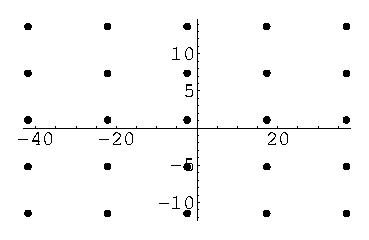
\includegraphics[width=0.4\textwidth]{fcv/function/log1_i_ipi}
    \end{center}
    \caption{Plot of the values.}
    \label{log1_i_ipi}
  \end{figure}
\end{Solution}
}








%% $\e^z = \imath$ $\cos z = \sin z$ $\tan^2 z = -1$
\solutions{
\begin{Solution}
  \label{solution ez = i}
  \begin{enumerate}
    %%
    %%
    %%
  \item
    \begin{gather*}
      \e^z = \imath 
      \\
      z = \log \imath 
      \\
      z = \ln |\imath| + \imath \arg(\imath) 
      \\
      z = \ln(1) + \imath \left( \frac{\pi}{2} + 2 \pi n \right), 
      \quad n \in \mathbb{Z} 
      \\
      \boxed{
        z =  \imath \frac{\pi}{2} + \imath 2 \pi n, \quad n \in \mathbb{Z} 
        }
    \end{gather*}
    %%
    %%
    %%
  \item
    We can solve the equation by writing the cosine and sine in terms of the 
    exponential.
    \begin{gather*}
      \cos z = \sin z 
      \\
      \frac{\e^{\imath z} + \e^{-\imath z}}{2} = \frac{\e^{\imath z} - \e^{-\imath z}}{\imath 2} 
      \\
      (1 + \imath) \e^{\imath z} = (-1 + \imath) \e^{-\imath z} 
      \\
      \e^{\imath 2 z} = \frac{-1 + \imath}{1 + \imath} 
      \\
      \e^{\imath 2 z}  = \imath 
      \\
      \imath 2 z = \log(\imath) 
      \\
      \imath 2 z = \imath \frac{\pi}{2} + \imath 2 \pi n, \quad n \in \mathbb{Z} 
      \\
      \boxed{
        z = \frac{\pi}{4} + \pi n, \quad n \in \mathbb{Z} 
        }
    \end{gather*}
    %%
    %%
    %%
  \item
    \begin{gather*}
      \tan^2 z = -1 
      \\
      \sin^2 z = - \cos^2 z 
      \\
      \cos z = \pm \imath \sin z 
      \\
      \frac{\e^{\imath z} + \e^{-\imath z}}{2} = \pm \imath \frac{\e^{\imath z} - \e^{-\imath z}}{\imath 2} 
      \\
      \e^{-\imath z} = - \e^{-\imath z} \quad \mathrm{or} \quad \e^{\imath z} = - \e^{\imath z} 
      \\
      \e^{-\imath z} = 0 \quad \mathrm{or} \quad \e^{\imath z} = 0 
      \\
      \e^{y - \imath x} = 0 \quad \mathrm{or} \quad \e^{-y + \imath x} = 0 
      \\
      \e^y = 0 \quad \mathrm{or} \quad \e^{-y} = 0 
      \\
      \boxed{
        z = \emptyset
        }
    \end{gather*}
    There are no solutions for finite $z$.
  \end{enumerate}
\end{Solution}
}




%% \tan^{-1}(z) =\frac{\imath}{2} \log\left( \frac{i+z}{i-z}\right)
\solutions{
\begin{Solution}
  \label{solution arctan z}
  \begin{enumerate}
  \item
    \begin{gather*}
      w = \arctan(z) 
      \\
      z = \tan(w) 
      \\
      z = \frac{ \sin(w) }{ \cos(w) } 
      \\
      z = \frac{ \left( \e^{\imath w} - \e^{-\imath w} \right)/(\imath 2) }
      { \left( \e^{\imath w} + \e^{-\imath w} \right)/2 } 
      \\
      z \e^{\imath w} + z \e^{-\imath w} = - \imath \e^{\imath w} + \imath \e^{-\imath w} 
      \\
      (\imath + z) \e^{\imath 2 w} = (\imath - z) 
      \\
      \e^{\imath w} = \left( \frac{\imath - z}{\imath + z} \right)^{1/2} 
      \\
      w = - \imath \log \left( \frac{\imath - z}{\imath + z} \right)^{1/2} 
      \\
      \boxed{
        \arctan(z) = \frac{\imath}{2} \log \left( \frac{\imath + z}{\imath - z} \right) 
        }
    \end{gather*}
    We identify the branch points of the arctangent.
    \[
    \arctan(z) = \frac{\imath}{2} \left( \log( \imath + z ) - \log( \imath - z ) \right)
    \]
    There are branch points at $z = \pm \imath$ due to the logarithm terms.
    We examine the point at infinity with the change of variables 
    $\zeta = 1 / z$.
    \begin{gather*}
      \arctan(1/\zeta) = \frac{\imath}{2} \log \left( \frac{\imath + 1/\zeta}{\imath - 1/\zeta} \right) 
      \\
      \arctan(1/\zeta) = \frac{\imath}{2} \log \left( \frac{\imath \zeta + 1}{\imath \zeta - 1} \right) 
    \end{gather*}
    As $\zeta \to 0$, the argument of the logarithm term tends to $-1$  The 
    logarithm does not have a branch point at that point.
    Since $\arctan(1/\zeta)$ does not have a branch point at $\zeta = 0$,
    $\arctan(z)$ does not have a branch point at infinity.
    %%
  \item
    \begin{gather*}
      w = \arctanh(z) 
      \\
      z = \tanh(w) 
      \\
      z = \frac{ \sinh(w) }{ \cosh(w) } 
      \\
      z = \frac{ \left( \e^{w} - \e^{-w} \right)/2 }
      { \left( \e^{w} + \e^{-w} \right)/2 } 
      \\
      z \e^{w} + z \e^{-w} = \e^{w} - \e^{-w} 
      \\
      (z - 1) \e^{2 w} = -z - 1 
      \\
      \e^w = \left( \frac{-z - 1}{z - 1} \right)^{1/2} 
      \\
      w = \log \left( \frac{z + 1}{1 - z} \right)^{1/2} 
      \\
      \boxed{
        \arctanh(z) = \frac{1}{2} \log \left( \frac{1 + z}{1 - z} \right) 
        }
    \end{gather*}
    We identify the branch points of the hyperbolic arctangent.
    \[
    \arctanh(z) = \frac{1}{2} \left( \log(1 + z) - \log(1 - z) \right)
    \]
    There are branch points at $z = \pm 1$ due to the logarithm terms.
    We examine the point at infinity with the change of variables 
    $\zeta = 1 / z$.
    \begin{gather*}
      \arctanh(1/\zeta) = \frac{1}{2} \log \left( \frac{1 + 1/\zeta}{1 - 1/\zeta} \right) 
      \\
      \arctanh(1/\zeta) = \frac{1}{2} \log \left( \frac{\zeta + 1}{\zeta - 1} \right) 
    \end{gather*}
    As $\zeta \to 0$, the argument of the logarithm term tends to $-1$  The 
    logarithm does not have a branch point at that point.
    Since $\arctanh(1/\zeta)$ does not have a branch point at $\zeta = 0$,
    $\arctanh(z)$ does not have a branch point at infinity.
    %%
  \item
  \begin{gather*}
    w = \arccosh(z)
    \\
    z = \cosh(w)
    \\
    z = \frac{ \e^w + \e^{-w} }{2}
    \\
    \e^{2 w} - 2 z \e^w + 1 = 0
    \\
    \e^w = z + \left( z^2 - 1 \right)^{1/2}
    \\
    w = \log \left( z + \left( z^2 - 1 \right)^{1/2} \right)
    \\
    \boxed{
      \arccosh(z) = \log \left( z + \left( z^2 - 1 \right)^{1/2} \right)
      }
  \end{gather*}
  We identify the branch points of the hyperbolic arc-cosine.
  \[
  \arccosh(z) = \log \left( z + (z - 1)^{1/2} (z + 1)^{1/2} \right)
  \]
  First we consider branch points due to the square root.
  There are branch points at $z = \pm 1$ due to the square root terms.
  If we walk around the singularity at $z = 1$ and no other singularities,
  the $\left( z^2 - 1 \right)^{1/2}$ term changes sign.  This will change the
  value of $\arccosh(z)$.  The same is true for the point $z = -1$.
  The point at infinity is not a branch point for $\left( z^2 - 1 \right)^{1/2}$.
  We factor the expression to verify this.
  \[
  \left( z^2 - 1 \right)^{1/2}
  = \left( z^2 \right)^{1/2} \left( 1 - z^{-2} \right)^{1/2}
  \]
  $\left( z^2 \right)^{1/2}$ does not have a branch point at infinity.  It is 
  multi-valued, but it has no branch points.
  $\left( 1 - z^{-2} \right)^{1/2}$ does not have a branch point at infinity,
  The argument of the square root function tends to unity there.
  In summary, there are branch points at $z = \pm 1$ due to the square root.
  If we walk around either one of the these branch points. the square root
  term will change value.  If we walk around both of these points, the square 
  root term will not change value.

  Now we consider branch points due to logarithm.  There may be branch 
  points where the argument of the logarithm vanishes or tends to infinity.
  We see if the argument of the logarithm vanishes.
  \begin{gather*}
    z + \left( z^2 - 1 \right)^{1/2} = 0
    \\
    z^2 = z^2 - 1
  \end{gather*}
  $z + \left( z^2 - 1 \right)^{1/2}$ is non-zero and finite everywhere in 
  the complex plane.  The only possibility for a branch point in the 
  logarithm term is the point at infinity.  We see if the argument of 
  $z + \left( z^2 - 1 \right)^{1/2}$ changes when we walk around infinity
  but no other singularity.  We consider a circular path with center at the
  origin and radius greater than unity.  We can either say that this path
  encloses the two branch points at $z = \pm 1$ and no other singularities
  or we can say that this path encloses the point at infinity and no other 
  singularities.  We examine the value of the argument of the logarithm 
  on this path.
  \[
  z + \left( z^2 - 1 \right)^{1/2} 
  = z + \left( z^2 \right)^{1/2} \left( 1 - z^{-2} \right)^{1/2} 
  \]
  Neither $\left( z^2 \right)^{1/2}$ nor $\left( 1 - z^{-2} \right)^{1/2}$ changes 
  value as we walk the path.  Thus we can use the principal branch of the 
  square root in the expression.
  \[
  z + \left( z^2 - 1 \right)^{1/2} 
  = z \pm z \sqrt{1 - z^{-2}}
  = z \left( 1 \pm \sqrt{1 - z^{-2}} \right)
  \]

  First consider the ``$+$'' branch.
  \[
  z \left( 1 + \sqrt{1 - z^{-2}} \right)
  \]
  As we walk the path around infinity, the argument of $z$ changes by $2 \pi$
  while the argument of $\left( 1 + \sqrt{1 - z^{-2}} \right)$ does not change.
  Thus the argument of $z + \left( z^2 - 1 \right)^{1/2}$ changes by $2 \pi$ when 
  we go around infinity.  This makes the value of the logarithm change by 
  $\imath 2 \pi$.  There is a branch point at infinity.

  First consider the ``$-$'' branch.
  \begin{align*}
    z \left( 1 - \sqrt{1 - z^{-2}} \right)
    &= z \left( 1 - \left(1 - \frac{1}{2} z^{-2} 
        + \mathcal{O}\left(z^{-4} \right) \right) \right)
    \\
    &= z \left( \frac{1}{2} z^{-2} + \mathcal{O}\left(z^{-4} \right) \right)
    \\
    &= \frac{1}{2} z^{-1} \left( 1 + \mathcal{O}\left(z^{-2} \right) \right)
  \end{align*}
  As we walk the path around infinity, the argument of $z^{-1}$ changes by $-2 \pi$
  while the argument of $\left( 1 + \mathcal{O}\left(z^{-2} \right) \right)$ 
  does not change.
  Thus the argument of $z + \left( z^2 - 1 \right)^{1/2}$ changes by $-2 \pi$ when 
  we go around infinity.  This makes the value of the logarithm change by 
  $-\imath 2 \pi$.  Again we conclude that there is a branch point at infinity.

  For the sole purpose of overkill, let's repeat the above analysis from a 
  geometric viewpoint.  Again we consider the possibility of a branch point
  at infinity due to the logarithm.  We walk along the circle shown in 
  the first plot of Figure~\ref{figure map-z11z2}.  Traversing this path, 
  we go around infinity, but no other singularities.  We consider the 
  mapping $w = z + \left( z^2 - 1 \right)^{1/2}$.  Depending on the branch of the 
  square root, the circle is mapped to one one of the contours shown in the 
  second plot.  For each branch, the argument of $w$ changes by $\pm 2 \pi$ as 
  we traverse the circle in the $z$-plane.  Therefore the value of 
  $\arccosh(z) = \log \left( z + \left( z^2 - 1 \right)^{1/2} \right)$ changes 
  by $\pm \imath 2 \pi$ as we traverse the circle.  We again conclude that there 
  is a branch point at infinity due to the logarithm.
  \begin{figure}[htbp!]
    \begin{center}
      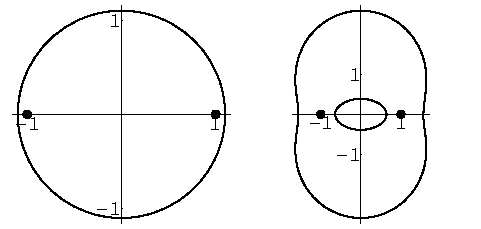
\includegraphics[width=0.5\textwidth]{fcv/function/map-z11z2}
    \end{center}
    \caption{The mapping of a circle.}
    \label{figure map-z11z2}
  \end{figure}

  To summarize:  There are branch points at $z = \pm 1$ due to the square root
  and a branch point at infinity due to the logarithm.
  \end{enumerate}
\end{Solution}
}








\solutions{
%%-----------------------------------------------------------------------------
\begin{large}
  \noindent
  \textbf{Branch Points and Branch Cuts}
\end{large}
}






\solutions{
\begin{Solution}
  \label{solution log zz+1z-1}
  We expand the function to diagnose the branch points in the finite complex
  plane.
  \[
  f(z) = \log \left( \frac{ z (z+1) }{ z-1 } \right)
  = \log(z) + \log(z+1) - \log(z-1)
  \]
  The are branch points at $z = -1,0,1$.  Now we examine the point at 
  infinity.  We make the change of variables $z = 1 / \zeta$.
  \begin{align*}
    f \left( \frac{1}{\zeta} \right) 
    &= \log \left( \frac{ (1 / \zeta) (1 / \zeta + 1) }{ (1 / \zeta - 1) } \right)
    \\
    &= \log \left( \frac{1}{\zeta}  \frac{ (1 + \zeta }{ 1 - \zeta } \right)
    \\
    &= \log(1 + \zeta) - \log(1 - \zeta) - \log(\zeta)
  \end{align*}
  $\log(\zeta)$ has a branch point at $\zeta = 0$.  The other terms do not have
  branch points there.  Since $f(1 / \zeta)$ has a branch point at $\zeta = 0$
  $f(z)$ has a branch point at infinity.

  Note that in walking around either $z = -1$ or $z = 0$ once in the 
  positive direction, the argument of $z (z+1) / (z-1)$ changes by
  $2 \pi$.  In walking around $z = 1$, the argument of $z (z+1) / (z-1)$ 
  changes by $-2 \pi$.  This argument does not change if we walk around
  both $z = 0$ and $z = 1$.  Thus we put a branch cut between $z = 0$ and 
  $z = 1$.  Next be put a branch cut between $z = -1$ and the point at
  infinity.  This prevents us from walking around either of these branch 
  points.  These two branch cuts separate the branches of the function.
  See Figure~\ref{figure branch-cuts-logzz1z1}
  \begin{figure}[htbp!]
    \begin{center}
      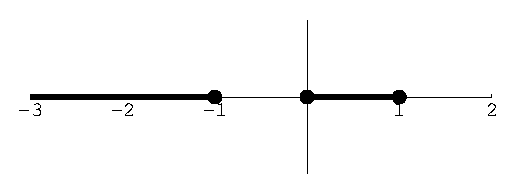
\includegraphics[width=0.5\textwidth]{fcv/function/branch-cuts-logzz1z1}
    \end{center}
    \caption{The branch cuts.}
    \label{figure branch-cuts-logzz1z1}
  \end{figure}
\end{Solution}
}








\solutions{
\begin{Solution}
  \label{solution z3 z2 6z 12}
  First we factor the function.
  \[
  f(z) = \left( z (z + 3) (z - 2) \right)^{1/2} 
  = z^{1/2}  (z + 3)^{1/2}  (z - 2)^{1/2}
  \]
  There are branch points at $z = -3, 0, 2$.  Now we examine the point at 
  infinity.
  \[
  f \left( \frac{1}{\zeta} \right) 
  = \left( \frac{1}{\zeta} 
    \left( \frac{1}{\zeta} + 3 \right) 
    \left( \frac{1}{\zeta} - 2 \right) \right)^{1/2}
  = \zeta^{-3/2}  ( ( 1 + 3 \zeta )  ( 1 - 2 \zeta ) )^{1/2}
  \]
  Since $\zeta^{-3/2}$ has a branch point at $\zeta = 0$  and the rest of the
  terms are analytic there, $f(z)$ has a branch point at infinity.

  Consider the set of branch cuts in Figure~\ref{figure bpz3z26z}.  
  These cuts do not permit us to walk around any single branch point.
  We can only walk around none or all of the branch points, (which is 
  the same thing).  The cuts can be used to define a single-valued 
  branch of the function.

  \begin{figure}[htbp!]
    \begin{center}
      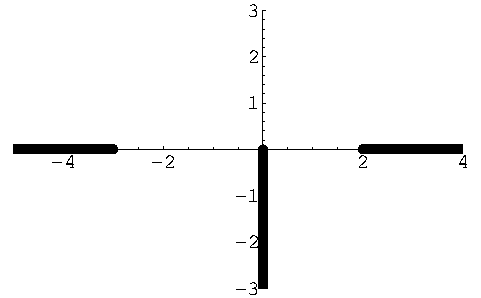
\includegraphics[width=0.5\textwidth]{fcv/function/bpz3z26z}
    \end{center}
    \caption{The branch cuts.}
    \label{figure bpz3z26z}
  \end{figure}

  Now to define the branch.  We make a choice of angles.
  \begin{align*}
    z+3 &= r_1 \e^{\imath \theta_1}, \quad -\pi < \theta_1 < \pi
    \\
    z &= r_2 \e^{\imath \theta_2}, \quad - \frac{\pi}{2} < \theta_2 < \frac{3 \pi}{2}
    \\
    z-2 &= r_3 \e^{\imath \theta_3}, \quad 0 < \theta_3 < 2 \pi
  \end{align*}
  The function is
  \[
  f(z) = \left( r_1 \e^{\imath \theta_1} r_2 \e^{\imath \theta_2} r_3 \e^{\imath \theta_3} \right)^{1/2}
  = \sqrt{ r_1 r_2 r_3 } \e^{\imath \left( \theta_1 + \theta_2 + \theta_3 \right)/2 }.
  \]
  We evaluate the function at $z = -1$.
  \[
  f(-1) = \sqrt{ (2) (1) (3) } \e^{\imath (0 + \pi + \pi) / 2} = - \sqrt{6}
  \]
  We see that our choice of angles gives us the desired branch.



  The stereographic projection is the projection from the complex plane 
  onto a unit sphere with south pole at the origin.  The point $z = x + \imath y$
  is mapped to the point $(X,Y,Z)$ on the sphere with
  \[
  X = \frac{4 x}{|z|^2 + 4}, \quad
  Y = \frac{4 y}{|z|^2 + 4}, \quad
  Z = \frac{2 |z|^2}{|z|^2 + 4}.
  \]
  Figure~\ref{figure bp-stereographic-z3z26z12} first shows the branch
  cuts and their stereographic projections and then shows the stereographic
  projections alone.
  \begin{figure}[htbp!]
    \begin{center}
      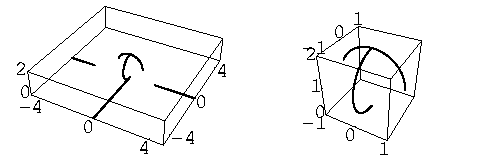
\includegraphics[width=0.5\textwidth]{fcv/function/bp-stereographic-z3z26z12}
    \end{center}
    \caption{The branch cuts and their stereographic projections.}
    \label{figure bp-stereographic-z3z26z12}
  \end{figure}
\end{Solution}
}







\solutions{
\begin{Solution}
  \label{solution mapping z13}
  \begin{enumerate}
    %%
  \item 
    For each value of $z$, $f(z) = z^{1/3}$ has three values.
    \[
    f(z) = z^{1/3} = \sqrt[3]{z} \e^{\imath k 2 \pi/3}, \quad k = 0,1,2
    \]
    %%
  \item
    \[
    g(w) = w^3 = |w|^3 \e^{\imath 3 \arg(w)}
    \]
    Any sector of the $w$ plane of angle $2 \pi/3$ maps one-to-one to the whole 
    $z$-plane.
    \begin{gather*}
      g : \left\{ r \e^{\imath \theta} \mid r \geq 0, \theta_0 \leq \theta < \theta_0 + 2 \pi/3 \right\} 
      \mapsto \left\{ r^3 \e^{\imath 3 \theta} \mid r \geq 0, \theta_0 \leq \theta < \theta_0 + 2 \pi/3 \right\} 
      \\
      g : \left\{ r \e^{\imath \theta} \mid r \geq 0, \theta_0 \leq \theta < \theta_0 + 2 \pi/3 \right\} 
      \mapsto \left\{ r \e^{\imath \theta} \mid r \geq 0, 3 \theta_0 \leq \theta < 3 \theta_0 + 2 \pi \right\} 
      \\
      g : \left\{ r \e^{\imath \theta} \mid r \geq 0, \theta_0 \leq \theta < \theta_0 + 2 \pi/3 \right\} 
      \mapsto \mathbb{C}
    \end{gather*}
    See Figure~\ref{figure sector-z3} to see how $g(w)$ maps the 
    sector $0 \leq \theta < 2 \pi/3$.
    \begin{figure}[htbp!]
      \begin{center}
        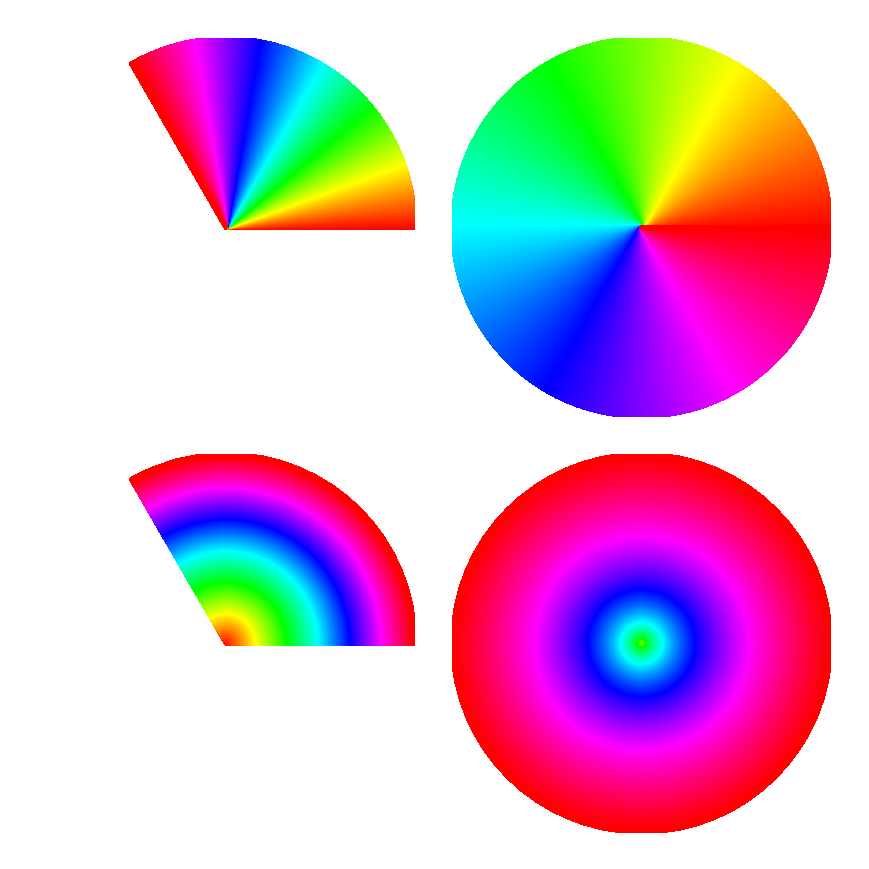
\includegraphics[width=0.5\textwidth]{fcv/function/sector-z3}
      \end{center}
      \caption{The function maps the sector 
        one-to-one to the whole complex plane.}
      \label{figure sector-z3}
    \end{figure}
    %%
  \item
    See Figure~\ref{figure riemann-surface-z13} for a depiction of the 
    Riemann surface for $f(z) = z^{1/3}$.  We show two views of the surface
    and a curve that traces the edge of the shown portion of the surface.
    The depiction is misleading because the surface is not self-intersecting.
    We would need four dimensions to properly visualize the this Riemann 
    surface.
    \begin{figure}[htbp!]
      \begin{center}
        \includegraphics[width=0.8\textwidth]{fcv/function/riemann-surface-z13}
      \end{center}
      \caption{The Riemann surface.}
      \label{figure riemann-surface-z13}
    \end{figure}
    %%
  \item
    $f(z) = z^{1/3}$ has branch points at $z = 0$ and $z = \infty$.  Any branch cut 
    which connects these two points would prevent us from walking around
    the points singly and would thus separate the branches of the function.
    For example, we could put a branch cut on the negative real axis.
    Defining the angle $-\pi < \theta < \pi$ for the mapping
    \[
    f \left( r \e^{\imath \theta} \right) = \sqrt[3]{r} \e^{\imath \theta/3}
    \]
    defines a single-valued branch of the function.
  \end{enumerate}
\end{Solution}
}







%% f(z)=(z^3-1)^{1/2}.
\solutions{
\begin{Solution}
  \label{solution z3112}
  The cube roots of $1$ are 
  \[
  \left\{ 1, \e^{\imath 2 \pi / 3}, \e^{\imath 4 \pi / 3} \right\}
  =
  \left\{ 1, \frac{-1 + \imath \sqrt{3}}{2}, \frac{-1 - \imath \sqrt{3}}{2} \right\}.
  \]
  We factor the polynomial.
  \[
  \left( z^3 - 1 \right)^{1/2}
  = (z - 1)^{1/2} \left( z + \frac{1 - \imath \sqrt{3}}{2} \right)^{1/2} 
  \left( z + \frac{1 + \imath \sqrt{3}}{2} \right)^{1/2}
  \]
  There are branch points at each of the cube roots of unity.
  \[
  z = \left\{ 1, \frac{-1 + \imath \sqrt{3}}{2}, \frac{-1 - \imath \sqrt{3}}{2} \right\}
  \]
  Now we examine the point at infinity.  We make the change of variables 
  $z = 1 / \zeta$.
  \[
  f(1/ \zeta) = \left( 1 / \zeta^3 - 1 \right)^{1/2} = \zeta^{-3/2}  \left( 1 - \zeta^3 \right)^{1/2}
  \]
  $\zeta^{-3/2}$ has a branch point at $\zeta = 0$, while $\left( 1 - \zeta^3 \right)^{1/2}$ 
  is not singular there.
  Since $f(1 / \zeta)$ has a branch point at $\zeta = 0$, $f(z)$ has a branch point
  at infinity.

  There are several ways of introducing branch cuts to separate the
  branches of the function.  The easiest approach is to put a branch
  cut from each of the three branch points in the finite complex plane
  out to the branch point at infinity.  See
  Figure~\ref{bc_sqrt_z3_1}a.  Clearly this makes the function single
  valued as it is impossible to walk around any of the branch points.
  Another approach is to have a branch cut from one of the branch
  points in the finite plane to the branch point at infinity and a
  branch cut connecting the remaining two branch points.  See
  Figure~\ref{bc_sqrt_z3_1}bcd.  Note that in walking around any one
  of the finite branch points, (in the positive direction), the
  argument of the function changes by $\pi$.  This means that the value
  of the function changes by $\e^{\imath \pi}$, which is to say the value
  of the function changes sign.  In walking around any two of the
  finite branch points, (again in the positive direction), the
  argument of the function changes by $2 \pi$.  This means that the
  value of the function changes by $\e^{\imath 2 \pi}$, which is to say
  that the value of the function does not change.  This demonstrates
  that the latter branch cut approach makes the function
  single-valued.

  \begin{figure}[htbp!]
    \begin{center}
      \includegraphics[width=0.7\textwidth]{fcv/function/bc_sqrt_z3_1}
    \end{center}
    \caption{Suitable branch cuts.}
    \label{bc_sqrt_z3_1}
  \end{figure}




  Now we construct a branch.  We will use the branch cuts in
  Figure~\ref{bc_sqrt_z3_1}a.  We introduce variables to measure radii and
  angles from the three finite branch points.
  \begin{gather*}
    z - 1 = r_1 \e^{\imath \theta_1}, \quad 0 < \theta_1 < 2 \pi 
    \\
    z + \frac{1 - \imath \sqrt{3}}{2} = r_2 \e^{\imath \theta_2}, 
    \quad -\frac{2 \pi}{3} < \theta_2 < \frac{\pi}{3} 
    \\
    z + \frac{1 + \imath \sqrt{3}}{2} = r_3 \e^{\imath \theta_3},
    \quad -\frac{\pi}{3} < \theta_3 < \frac{2 \pi}{3}
  \end{gather*}
  We compute $f(0)$ to see if it has the desired value.
  \begin{gather*}
    f(z) = \sqrt{r_1 r_2 r_3} \e^{\imath \left( \theta_1 + \theta_2 + \theta_3 \right) / 2} 
    \\
    f(0) = \e^{\imath (\pi - \pi / 3 + \pi / 3) / 2} = \imath
  \end{gather*}
  Since it does not have the desired value, we change the range of $\theta_1$.
  \[
  z - 1 = r_1 \e^{\imath \theta_1}, \quad 2 \pi < \theta_1 < 4 \pi
  \]
  $f(0)$ now has the desired value.
  \[
  f(0) = \e^{\imath (3 \pi - \pi / 3 + \pi / 3) / 2} = - \imath
  \]
  We compute $f(-1)$.
  \[
  f(-1) = \sqrt{2} \e^{\imath (3 \pi - 2 \pi / 3 + 2 \pi / 3) / 2} = - \imath \sqrt{2}
  \]
\end{Solution}
}






%% w(z) = \left( (z-1)(z-6)(z+2) \right)^{1/2}
\solutions{
\begin{Solution}
  \label{solution z1z6z2}
  First we factor the function.
  \[
  w(z) = \left( (z+2) (z-1) (z-6) \right)^{1/2} 
  = (z+2)^{1/2}  (z-1)^{1/2}  (z-6)^{1/2}
  \]
  There are branch points at $z = -2,1,6$.  Now we examine the point at 
  infinity.
  \[
  w \left( \frac{1}{\zeta} \right) 
  = \left( \left( \frac{1}{\zeta} + 2 \right) 
    \left( \frac{1}{\zeta} - 1 \right) 
    \left( \frac{1}{\zeta} - 6 \right) \right)^{1/2}
  = \zeta^{-3/2}  \left( \left( 1 + \frac{2}{\zeta} \right) 
    \left( 1 - \frac{1}{\zeta} \right) 
    \left( 1 - \frac{6}{\zeta} \right) \right)^{1/2}
  \]
  Since $\zeta^{-3/2}$ has a branch point at $\zeta = 0$  and the rest of the
  terms are analytic there, $w(z)$ has a branch point at infinity.

  Consider the set of branch cuts in Figure~\ref{bpz216}.  These cuts
  let us walk around the branch points at $z = -2$ and $z = 1$
  together or if we change our perspective, we would be walking around
  the branch points at $z = 6$ and $z = \infty$ together.  Consider a
  contour in this cut plane that encircles the branch points at $z =
  -2$ and $z = 1$.  Since the argument of $\left( z-z_0 \right)^{1/2}$ changes by
  $\pi$ when we walk around $z_0$, the argument of $w(z)$ changes by
  $2 \pi$ when we traverse the contour.  Thus the value of the
  function does not change and it is a valid set of branch cuts.

  \begin{figure}[htbp!]
    \begin{center}
      \includegraphics[width=0.4\textwidth]{fcv/function/bpz216}
    \end{center}
    \caption{The branch cuts.}
    \label{bpz216}
  \end{figure}


  Now to define the branch.  We make a choice of angles.
  \begin{align*}
    z+2 &= r_1 \e^{\imath \theta_1}, \quad \theta_1 = \theta_2\ \mathrm{for}\ z \in (1 \ldots 6), 
    \\
    z-1 &= r_2 \e^{\imath \theta_2}, \quad \theta_2 = \theta_1\ \mathrm{for}\ z \in (1 \ldots 6), 
    \\
    z-6 &= r_3 \e^{\imath \theta_3}, \quad 0 < \theta_3 < 2 \pi
  \end{align*}
  The function is
  \[
  w(z) = \left( r_1 \e^{\imath \theta_1} r_2 \e^{\imath \theta_2} r_3 \e^{\imath \theta_3} \right)^{1/2}
  = \sqrt{ r_1 r_2 r_3 } \e^{\imath \left( \theta_1 + \theta_2 + \theta_3 \right)/2 }.
  \]
  We evaluate the function at $z = 4$.
  \[
  w(4) = \sqrt{ (6) (3) (2) } \e^{\imath (2 \pi n + 2 \pi n + \pi) / 2} = \imath 6
  \]
  We see that our choice of angles gives us the desired branch.
\end{Solution}
}







%% \cos z^{1/2} (z + \imath)^{-z}
\solutions{
\begin{Solution}
  \label{solution cos z12}
  \begin{enumerate}
  \item 
    \[
    \cos \left( z^{1/2} \right) 
    = \cos\left( \pm \sqrt{z} \right) 
    = \cos\left( \sqrt{z} \right)
    \]
    This is a single-valued function.  There are no branch points.
  \item 
    \begin{align*}
      (z + \imath)^{-z}
      &= \e^{-z \log(z + \imath) } 
      \\
      &= \e^{-z (\ln |z + \imath| + \imath \Arg(z + \imath) + \imath 2 \pi n) }, \quad n \in \mathbb{Z} 
    \end{align*}
    There is a branch point at $z = - \imath$.  There are an infinite number of 
    branches.
  \end{enumerate}
\end{Solution}
}








%%
\solutions{
\begin{Solution}
  \label{solution z2112}
  \begin{enumerate}
    %%
  \item
    \[
    f(z) = \left( z^2 + 1 \right)^{1/2} = (z + \imath)^{1/2}  (z - \imath)^{1/2}
    \]
    We see that there are branch points at $z = \pm \imath$.
    To examine the point at infinity, we substitute $z = 1/\zeta$ and examine
    the point $\zeta = 0$.
    \[
    \left( \left( \frac{1}{\zeta} \right)^2 + 1 \right)^{1/2}
    = \frac{1}{\left( \zeta^2 \right)^{1/2}}  \left( 1 + \zeta^2 \right)^{1/2}
    \]
    Since there is no branch point at $\zeta = 0$, $f(z)$ has no branch point at
    infinity.

    A branch cut connecting $z = \pm \imath$ would make the function single-valued.
    We could also accomplish this with two branch cuts starting $z = \pm \imath$
    and going to infinity.
    %%
  \item
    \[
    f(z) = \left( z^3 - z \right)^{1/2} = z^{1/2}  (z-1)^{1/2}  (z+1)^{1/2}
    \]
    There are branch points at $z = -1,0,1$.  Now we consider the point at
    infinity.
    \[
    f\left( \frac{1}{\zeta} \right)
    = \left( \left(\frac{1}{\zeta}\right)^3 - \frac{1}{\zeta} \right)^{1/2}
    = \zeta^{-3/2}  \left( 1 - \zeta^2 \right)^{1/2}
    \]
    There is a branch point at infinity.

    One can make the function single-valued with three branch cuts that start
    at $z = -1,0,1$ and each go to infinity.  We can also make the function
    single-valued with a branch cut that connects two of the points
    $z = -1,0,1$ and another branch cut that starts at the remaining point
    and goes to infinity.
    %%
  \item
    \[
    f(z) = \log \left( z^2 - 1 \right) = \log (z-1) + \log (z+1)
    \]
    There are branch points at $z = \pm 1$.
    \[
    f \left( \frac{1}{\zeta} \right)
    = \log \left( \frac{1}{\zeta^2} - 1 \right)
    = \log \left( \zeta^{-2} \right) + \log \left( 1 - \zeta^2 \right)
    \]
    $\log \left( \zeta^{-2} \right)$ has a branch point at $\zeta = 0$.
    \[
    \log \left( \zeta^{-2} \right) = \ln \left| \zeta^{-2} \right| 
    + \imath \arg\left( \zeta^{-2} \right)
    = \ln \left| \zeta^{-2} \right| - \imath 2 \arg(\zeta)
    \]
    Every time we walk around the point $\zeta = 0$ in the positive direction,
    the value of the function changes by $-\imath 4 \pi$.  $f(z)$ has a branch point
    at infinity.

    We can make the function single-valued by introducing two branch cuts that
    start at $z = \pm 1$ and each go to infinity.
    %%
  \item
    \[
    f(z) = \log \left( \frac{z+1}{z-1} \right)
    = \log (z+1) - \log (z-1)
    \]
    There are branch points at $z = \pm 1$.
    \[
    f \left( \frac{1}{\zeta} \right)
    = \log \left( \frac{1/\zeta + 1}{1/\zeta - 1} \right)
    = \log \left( \frac{1 + \zeta}{1 - \zeta} \right)
    \]
    There is no branch point at $\zeta = 0$.  $f(z)$ has no branch point at
    infinity.

    We can make the function single-valued by introducing two branch cuts that
    start at $z = \pm 1$ and each go to infinity.  We can also make the function
    single-valued with a branch cut that connects the points $z = \pm 1$.
    This is because $\log(z+1)$ and $-\log(z-1)$ change by $\imath 2 \pi$ and
    $- \imath 2 \pi$, respectively, when you walk around their branch points once
    in the positive direction.
  \end{enumerate}
\end{Solution}
}












%% f(z) = \left( z^3 + 8 \right)^{1/2}
\solutions{
\begin{Solution}
  \label{solution z3812}
  \begin{enumerate}
    %%
    %%
    %%
  \item
    The cube roots of $-8$ are 
    \[
    \left\{ -2, -2 \e^{\imath 2 \pi / 3}, -2 \e^{\imath 4 \pi / 3} \right\}
    =
    \left\{ -2, 1 + \imath \sqrt{3}, 1 - \imath \sqrt{3} \right\}.
    \]
    Thus we can write
    \[
    \left( z^3 + 8 \right)^{1/2}
    = (z + 2)^{1/2}  \left( z - 1 - \imath \sqrt{3} \right)^{1/2}  
    \left( z - 1 + \imath \sqrt{3} \right)^{1/2}.
    \]
    There are three branch points on the circle of radius 2.
    \[
    z = \left\{ -2, 1 + \imath \sqrt{3}, 1 - \imath \sqrt{3} \right\}.
    \]
    We examine the point at infinity.
    \[
    f(1/ \zeta) = \left( 1 / \zeta^3 + 8 \right)^{1/2} = \zeta^{-3/2}  \left( 1 + 8 \zeta^3 \right)^{1/2}
    \]
    Since $f(1 / \zeta)$ has a branch point at $\zeta = 0$, $f(z)$ has a branch point
    at infinity.

    There are several ways of introducing branch cuts outside of the
    disk $|z| < 2$ to separate the branches of the function.  The
    easiest approach is to put a branch cut from each of the three
    branch points in the finite complex plane out to the branch point
    at infinity.  See Figure~\ref{bc_sqrt_z3_8}a.  Clearly this makes
    the function single valued as it is impossible to walk around any
    of the branch points.  Another approach is to have a branch cut
    from one of the branch points in the finite plane to the branch
    point at infinity and a branch cut connecting the remaining two
    branch points.  See Figure~\ref{bc_sqrt_z3_8}bcd.  Note that in
    walking around any one of the finite branch points, (in the
    positive direction), the argument of the function changes by $\pi$.
    This means that the value of the function changes by $\e^{\imath \pi}$,
    which is to say the value of the function changes sign.  In
    walking around any two of the finite branch points, (again in the
    positive direction), the argument of the function changes by $2 \pi$.  
    This means that the value of the function changes by $\e^{\imath 2 \pi}$, 
    which is to say that the value of the function does not
    change.  This demonstrates that the latter branch cut approach
    makes the function single-valued.

    \begin{figure}[htbp!]
      \begin{center}
        \includegraphics[width=0.8\textwidth]{fcv/function/bc_sqrt_z3_8}
      \end{center}
      \caption{Suitable branch cuts.}
      \label{bc_sqrt_z3_8}
    \end{figure}
    %%
    %%
    %%
  \item
    \[
    f(z) = \log \left( 5 + \left( \frac{z+1}{z-1} \right)^{1/2} \right)
    \]
    First we deal with the function
    \[
    g(z) = \left( \frac{z+1}{z-1} \right)^{1/2} 
    \]
    Note that it has branch points at $z = \pm 1$.  
    Consider the point at infinity.
    \[
    g(1 / \zeta) = \left( \frac{1 / \zeta + 1}{1 / \zeta - 1} \right)^{1/2} 
    = \left( \frac{1 + \zeta}{1 - \zeta} \right)^{1/2} 
    \]
    Since $g(1 / \zeta)$ has no branch point at $\zeta = 0$, $g(z)$ has no branch point
    at infinity.  This means that if we walk around both of the branch points
    at $z = \pm1$, the function does not change value.  We can verify this with
    another method:  When we walk around the
    point $z = -1$ once in the positive direction, the argument of $z+1$ 
    changes by $2 \pi$, the argument of $(z+1)^{1/2}$ changes by $\pi$
    and thus the value of $(z+1)^{1/2}$ changes by $\e^{\imath \pi} = -1$.
    When we walk around the
    point $z = 1$ once in the positive direction, the argument of $z - 1$ 
    changes by $2 \pi$, the argument of $(z-1)^{-1/2}$ changes by $-\pi$
    and thus the value of $(z-1)^{-1/2}$ changes by $\e^{-\imath \pi} = -1$.
    $f(z)$ has branch points at $z = \pm 1$.
    When we walk around both points $z = \pm 1$ once in the positive direction,
    the value of $\left( \frac{z+1}{z-1} \right)^{1/2}$ does not change.
    Thus we can make the function single-valued with a branch cut which 
    enables us to walk around either none or both of these branch points.
    We put a branch cut from $-1$ to $1$ on the real axis.

    %%A simple, closed curve separates the
    %%plane into a bounded and an unbounded region.  There is a duality in
    %%what such a curve encloses.  One can say that a curve goes around either
    %%the points in the bounded region or the unbounded region.  

    %%Recall that the function $\log z$ has branch point at $z = 0$ and at
    %%$z = \infty$.  The function is made single valued with any branch 
    %%cut connecting these two points.  
    %%Refer to Figure~\ref{two_paths}.  We can say that the first path
    %%either goes around the branch point at the origin, or the branch point
    %%at infinity.  The value of the logarithm changes in traversing such 
    %%a path.  The second path either encloses no branch points or encloses
    %%both the branch points.  The value of the logarithm does not change 
    %%on such a path.  In order for the value of the logarithm to change when
    %%traversing a simple, closed curve, one branch point must be on the ``inside'',
    %%and the other branch point must be on the ``outside''.

    %%\begin{figure}[htbp!]
    %%\begin{center}
    %%\includegraphics[width=0.4\textwidth]{fcv/function/two_paths}
    %%\end{center}
    %%\caption{Two paths in the complex plane.}
    %%\label{two_paths}
    %%\end{figure}

    $f(z)$ has branch points where
    \[
    5 + \left( \frac{z+1}{z-1} \right)^{1/2}
    \]
    is either zero or infinite.  The only place in the extended complex plane
    where the expression becomes infinite is at $z = 1$.  Now we look for 
    the zeros.
    \begin{gather*}
      5 + \left( \frac{z+1}{z-1} \right)^{1/2} = 0
      \\
      \left( \frac{z+1}{z-1} \right)^{1/2} = -5
      \\
      \frac{z+1}{z-1} = 25
      \\
      z + 1 = 25 z - 25 
      \\
      z = \frac{13}{12}
    \end{gather*}

    Note that 
    \[
    \left( \frac{13/12 + 1}{13/12 - 1} \right)^{1/2} = 25^{1/2} = \pm 5.
    \]
    On one branch, (which we call the positive branch), of the function $g(z)$
    the quantity 
    \[
    5 + \left( \frac{z+1}{z-1} \right)^{1/2}
    \]
    is always nonzero.  On the other (negative) branch of the function, 
    this quantity has a zero at $z = 13/12$.    

    %%On the positive branch of $g(z)$, $f(z)$ has no branch points 
    %%due to the logarithm.   This is because there is a point where 
    %%$5 + ((z+1)/(z-1))^{1/2}$ is infinite, but no point where it is zero.
    %%Thus no path could separate these points.  This branch needs no additional
    %%branch cuts to make $f(z)$ single-valued.

    %%On the negative branch of $g(z)$, $f(z)$ has branch points 
    %%at $z = 1$ and $z = 13/12$ due to the logarithm.   
    %%We make $f(z)$ single-valued with any branch cut which connects these 
    %%points.  We put a branch cut from $1$ to $13/12$ on the real axis.
    %%See Figure~\ref{log_5_etc} for the branch cuts on the positive and 
    %%negative branches of the square root.

    The logarithm introduces branch points at $z = 1$ on both the positive and
    negative branch of $g(z)$.  It introduces a branch point at $z = 13/12$ on
    the negative branch of $g(z)$.  To determine if additional branch cuts are
    needed to separate the branches, we consider 
    \[
    w = 5 + \left( \frac{z+1}{z-1} \right)^{1/2}
    \]
    and see where the branch cut
    between $\pm 1$ gets mapped to in the $w$ plane.  We rewrite the mapping.
    \[
    w = 5 + \left( 1 + \frac{2}{z-1} \right)^{1/2}
    \]
    The mapping is the following sequence of simple transformations:
    \begin{enumerate}
    \item $z \mapsto z - 1$
    \item $\displaystyle z \mapsto \frac{1}{z}$
    \item $z \mapsto 2 z$
    \item $z \mapsto z + 1$
    \item $\displaystyle z \mapsto z^{1/2}$
    \item $z \mapsto z + 5$
    \end{enumerate}
    We show these transformations graphically below.

    \includegraphics[height=1in]{fcv/function/5z1z1a}
    $z \mapsto z-1$
    \includegraphics[height=1in]{fcv/function/5z1z1b}
    $\displaystyle z \mapsto \frac{1}{z}$
    \includegraphics[height=1in]{fcv/function/5z1z1c}
    \\
    $z \mapsto 2 z$
    \includegraphics[height=1in]{fcv/function/5z1z1d}
    $z \mapsto z + 1$
    \includegraphics[height=1in]{fcv/function/5z1z1e}
    \\
    $\displaystyle z \mapsto z^{1/2}$
    \includegraphics[height=1in]{fcv/function/5z1z1f}
    $z \mapsto z + 5$
    \includegraphics[height=1in]{fcv/function/5z1z1g}

    For the positive branch of $g(z)$, the branch cut is mapped to the
    line $x = 5$ and the $z$ plane is mapped to the half-plane $x >
    5$.  $\log(w)$ has branch points at $w = 0$ and $w = \infty$.  It is
    possible to walk around only one of these points in the half-plane
    $x > 5$.  Thus no additional branch cuts are needed in the
    positive sheet of $g(z)$.

    For the negative branch of $g(z)$, the branch cut is mapped to the
    line $x = 5$ and the $z$ plane is mapped to the half-plane $x <
    5$.  It is possible to walk around either $w = 0$ or $w = \infty$
    alone in this half-plane.  Thus we need an additional branch cut.
    On the negative sheet of $g(z)$, we put a branch cut beteen $z =
    1$ and $z = 13/12$.  This puts a branch cut between $w = \infty$ and
    $w = 0$ and thus separates the branches of the logarithm.

    Figure~\ref{log_5_etc} shows the branch cuts in the positive and negative 
    sheets of $g(z)$.




    \begin{figure}[htbp!]
      \begin{center}
        \includegraphics[width=0.9\textwidth]{fcv/function/log_5_etc}
      \end{center}
      \caption{The branch cuts.}
      \label{log_5_etc}
    \end{figure}
    %%
    %%
    %%
  \item
    The function $f(z) = (z + \imath 3)^{1/2}$ has a branch point at $z = -\imath 3$.
    The function is made single-valued by connecting this point and the 
    point at infinity with a branch cut.
  \end{enumerate}
\end{Solution}
}








%% branch point at infinity I
\solutions{
\begin{Solution}
  \label{solution bp inf 1}
  Note that the curve with opposite orientation goes around infinity
  in the positive direction and does not enclose any branch points.  Thus 
  the value of the function does not change when traversing the curve, (with
  either orientation, of course).  This means that the argument of the function
  must change my an integer multiple of $2 \pi$.  Since the branch cut
  only allows us to encircle all three or none of the branch points, it
  makes the function single valued.
\end{Solution}
}



%% branch points at infinity II
\solutions{
\begin{Solution}
  \label{solution bp inf 2}
  We suppose that $f(z)$ has only one branch point in the finite complex
  plane.  Consider any contour that encircles this branch point in the positive
  direction.  $f(z)$ changes value if we traverse the contour.  If we reverse
  the orientation of the contour, then it encircles infinity in the positive
  direction, but contains no branch points in the finite complex plane.  Since
  the function changes value when we traverse the contour, we conclude that
  the point at infinity must be a branch point.  If $f(z)$ has only a 
  single branch point in the finite complex plane then it must have a 
  branch point at infinity.

  If $f(z)$ has two or more branch points in the finite complex plane then it
  may or may not have a branch point at infinity.  This is because the value 
  of the function may or may not change on a contour that encircles all the 
  branch points in the finite complex plane. 
\end{Solution}
}




%% $(z^4 + 1)^{1/4}
\solutions{
\begin{Solution}
  \label{solution z4114}
  First we factor the function,
  \[
  f(z) = \left( z^4 + 1 \right)^{1/4} 
  = \left( z - \frac{1 + \imath}{\sqrt{2}} \right)^{1/4} 
  \left( z - \frac{-1 + \imath}{\sqrt{2}} \right)^{1/4} 
  \left( z - \frac{-1 - \imath}{\sqrt{2}} \right)^{1/4} 
  \left( z - \frac{1 - \imath}{\sqrt{2}} \right)^{1/4}.
  \]
  There are branch points at $z = \frac{\pm 1 \pm \imath}{\sqrt{2}}$.  We make the
  substitution $z = 1/\zeta$ to examine the point at infinity.
  \begin{align*}
    f \left( \frac{1}{\zeta} \right) 
    &= \left( \frac{1}{\zeta^4} + 1 \right)^{1/4} 
    \\
    &= \frac{1}{\left( \zeta^4 \right)^{1/4} }  \left( 1 + \zeta^4 \right)^{1/4}
  \end{align*}
  $\left( \zeta^{1/4} \right)^4$ has a removable singularity at the point $\zeta = 0$, but
  no branch point there.  Thus $\left( z^4 + 1 \right)^{1/4}$ has no 
  branch point at infinity.

  Note that the argument of $\left( z^4 - z_0 \right)^{1/4}$ changes by 
  $\pi/2$ on a contour
  that goes around the point $z_0$ once in the positive direction.  
  The argument of $\left( z^4 + 1 \right)^{1/4}$ changes by $n \pi / 2$ on a contour
  that goes around $n$ of its branch points.  Thus any set of branch cuts 
  that permit you to walk around only one, two or three of the branch points
  will not make the function single valued.  A set of branch cuts that permit
  us to walk around only zero or all four of the branch points will make the
  function single-valued.   Thus we see that the first two sets of branch
  cuts in Figure~\ref{fourbc} will make the function single-valued, while
  the remaining two will not.

  %% CONTINUE: FIX
  Consider the contour in Figure~\ref{fourbc}.  There are two ways to
  see that the function does not change value while traversing the
  contour.  The first is to note that each of the branch points makes
  the argument of the function increase by $\pi/2$.  Thus the argument
  of $\left( z^4 + 1 \right)^{1/4}$ changes by $4 (\pi/2) = 2 \pi$ on the contour.
  This means that the value of the function changes by the factor
  $\e^{\imath 2 \pi} = 1$.  If we change the orientation of the contour,
  then it is a contour that encircles infinity once in the positive
  direction.  There are no branch points inside the this contour with
  opposite orientation.  (Recall that the inside of a contour lies to
  your left as you walk around it.)  Since there are no branch points
  inside this contour, the function cannot change value as we traverse
  it.
\end{Solution}
}








%%
\solutions{
\begin{Solution}
  \label{solution zz21}
  \[
  f(z) = \left( \frac{z}{z^2 + 1} \right)^{1/3}
  = z^{1/3}  (z - \imath)^{-1/3}  (z + \imath)^{-1/3}
  \]
  There are branch points at $z = 0, \pm \imath$.
  \[
  f \left( \frac{1}{\zeta} \right) =
  \left( \frac{1/\zeta}{(1/\zeta)^2 + 1} \right)^{1/3}
  = \frac{\zeta^{1/3}}{\left( 1 + \zeta^2 \right)^{1/3}}
  \]
  There is a branch point at $\zeta = 0$.  $f(z)$ has a branch point at
  infinity.

  We introduce branch cuts from $z = 0$ to infinity on the negative real axis,
  from $z = \imath$ to infinity on the positive imaginary axis and from $z = -\imath$
  to infinity on the negative imaginary axis.  As we cannot walk around any
  of the branch points, this makes the function single-valued.

  We define a branch by defining angles from the branch points.  Let
  \begin{alignat*}{2}
    z &= r \e^{\imath \theta} &\quad &-\pi < \theta < \pi, 
    \\
    (z - \imath) &= s \e^{\imath \phi} &\quad &-3 \pi/2 < \phi < \pi/2, 
    \\
    (z + \imath) &= t \e^{\imath \psi} &\quad &-\pi/2 < \psi < 3 \pi/2.
  \end{alignat*}
  With
  \begin{align*}
    f(z)
    &= z^{1/3}  (z - \imath)^{-1/3}  (z + \imath)^{-1/3} 
    \\
    &= \sqrt[3]{r} \e^{\imath \theta/3} 
    \frac{1}{\sqrt[3]{s}} \e^{-\imath \phi/3} 
    \frac{1}{\sqrt[3]{t}} \e^{-\imath \psi/3} 
    \\
    &= \sqrt[3]{ \frac{r}{s t} } \e^{ \imath (\theta - \phi - \psi) / 3}
  \end{align*}
  we have an explicit formula for computing the value of the function for this
  branch.  Now we compute $f(1)$ to see if we chose the correct ranges for the
  angles.  (If not, we'll just change one of them.)
  \[
  f(1) = \sqrt[3]{ \frac{1}{\sqrt{2} \sqrt{2}} }
  \e^{ \imath (0 - \pi/4 - (-\pi/4))/3}
  = \frac{1}{\sqrt[3]{2}}
  \]
  We made the right choice for the angles.  Now to compute $f(1 + \imath)$.
  \[
  f(1 + \imath) = \sqrt[3]{ \frac{\sqrt{2}}{1 \sqrt{5}} }
  \e^{\imath (\pi/4 - 0 - \Arctan(2))/3}
  = \sqrt[6]{ \frac{2}{5} } \e^{\imath (\pi/4  - \Arctan(2))/3}
  \]
  Consider the value of the function above and below the branch cut on the
  negative real axis.  Above the branch cut the function is
  \[
  f(-x + \imath 0) = \sqrt[3]{ \frac{x}{\sqrt{x^2+1} \sqrt{x^2+1}}} \e^{\imath (\pi - \phi - \psi)/3}
  \]
  Note that $\phi = - \psi$ so that
  \[
  f(-x + \imath 0) = \sqrt[3]{ \frac{x}{x^2+1} } \e^{\imath \pi/3}
  = \sqrt[3]{ \frac{x}{x^2+1} } \frac{1 + \imath \sqrt{3}}{2}.
  \]
  Below the branch cut $\theta = - \pi$ and
  \[
  f(-x - \imath 0) = \sqrt[3]{ \frac{x}{x^2+1} } \e^{\imath (-\pi )/3}
  = \sqrt[3]{ \frac{x}{x^2+1} } \frac{1 - \imath \sqrt{3}}{2}.
  \]
  For the branch cut along the positive imaginary axis,
  \begin{align*}
    f(\imath y + 0) &= \sqrt[3]{ \frac{y}{(y-1) (y+1)} } 
    \e^{\imath (\pi/2 - \pi/2 - \pi/2)/3} 
    \\
    &= \sqrt[3]{ \frac{y}{(y-1) (y+1)} } \e^{- \imath \pi/6} 
    \\
    &= \sqrt[3]{ \frac{y}{(y-1) (y+1)} } \frac{\sqrt{3} - \imath}{2},
  \end{align*}
  \begin{align*}
    f(\imath y - 0) &= \sqrt[3]{ \frac{y}{(y-1) (y+1)} } 
    \e^{\imath (\pi/2 - (-3 \pi/2) - \pi/2)/3} 
    \\
    &= \sqrt[3]{ \frac{y}{(y-1) (y+1)} } \e^{\imath \pi/2} 
    \\
    &= \imath \sqrt[3]{ \frac{y}{(y-1) (y+1)} }.
  \end{align*}
  For the branch cut along the negative imaginary axis,
  \begin{align*}
    f(-\imath y + 0) &= \sqrt[3]{ \frac{y}{(y+1) (y-1)} } 
    \e^{\imath (-\pi/2 - (-\pi/2) - (-\pi/2))/3} 
    \\
    &= \sqrt[3]{ \frac{y}{(y+1) (y-1)} }  \e^{\imath \pi/6} 
    \\
    &= \sqrt[3]{ \frac{y}{(y+1) (y-1)} }  \frac{\sqrt{3} + \imath}{2},
  \end{align*}
  \begin{align*}
    f(-\imath y - 0) &= \sqrt[3]{ \frac{y}{(y+1) (y-1)} } 
    \e^{\imath (-\pi/2 - (-\pi/2) - (3 \pi/2))/3} 
    \\
    &= \sqrt[3]{ \frac{y}{(y+1) (y-1)} }  \e^{- \imath \pi/2} 
    \\
    &= -\imath \sqrt[3]{ \frac{y}{(y+1) (y-1)} }.
  \end{align*}
\end{Solution}
}






%% ((z-1)(z-2)(z-3))^{1/2}
\solutions{
\begin{Solution}
  \label{solution z1z2z3}
  First we factor the function.
  \[
  f(z) = \left( (z-1) (z-2) (z-3) \right)^{1/2} 
  = (z-1)^{1/2} (z-2)^{1/2} (z-3)^{1/2}
  \]
  There are branch points at $z = 1,2,3$.  Now we examine the point 
  at infinity.
  \[
  f \left( \frac{1}{\zeta} \right) 
  = \left( \left( \frac{1}{\zeta} - 1 \right) 
    \left( \frac{1}{\zeta} - 2 \right) 
    \left( \frac{1}{\zeta} - 3 \right) \right)^{1/2}
  = \zeta^{-3/2} \left( \left( 1 - \frac{1}{\zeta} \right) 
    \left( 1 - \frac{2}{\zeta} \right) 
    \left( 1 - \frac{3}{\zeta} \right) \right)^{1/2}
  \]
  Since $\zeta^{-3/2}$ has a branch point at $\zeta = 0$  and the rest of the
  terms are analytic there, $f(z)$ has a branch point at infinity.

  The first two sets of branch cuts in Figure~\ref{bpbc123} do not
  permit us to walk around any of the branch points, including the
  point at infinity, and thus make the function single-valued.  The
  third set of branch cuts lets us walk around the branch points at $z
  = 1$ and $z = 2$ together or if we change our perspective, we would
  be walking around the branch points at $z = 3$ and $z = \infty$
  together.  Consider a contour in this cut plane that encircles the
  branch points at $z = 1$ and $z = 2$.  Since the argument of 
  $\left( z - z_0 \right)^{1/2}$ changes by $\pi$ when we walk around $z_0$, 
  the argument
  of $f(z)$ changes by $2 \pi$ when we traverse the contour.  Thus the
  value of the function does not change and it is a valid set of
  branch cuts.  Clearly the fourth set of branch cuts does not make
  the function single-valued as there are contours that encircle the
  branch point at infinity and no other branch points.  The other way
  to see this is to note that the argument of $f(z)$ changes by
  $3 \pi$ as we traverse a contour that goes around the branch points
  at $z = 1,2,3$ once in the positive direction.

  Now to define the branch.  We make the preliminary choice of angles,
  \begin{align*}
    z-1 &= r_1 \e^{\imath \theta_1}, \quad 0 < \theta_1 < 2 \pi, 
    \\
    z-2 &= r_2 \e^{\imath \theta_2}, \quad 0 < \theta_2 < 2 \pi, 
    \\
    z-3 &= r_3 \e^{\imath \theta_3}, \quad 0 < \theta_3 < 2 \pi.
  \end{align*}
  The function is
  \[
  f(z) = \left( r_1 \e^{\imath \theta_1} r_2 \e^{\imath \theta_2} r_3 \e^{\imath \theta_3} 
  \right)^{1/2}
  = \sqrt{ r_1 r_2 r_3 } \e^{\imath \left( \theta_1 + \theta_2 + \theta_3 \right)/2 }.
  \]
  The value of the function at the origin is
  \[
  f(0) = \sqrt{ 6 } \e^{\imath (3 \pi)/2} = - \imath \sqrt{6},
  \]
  which is not what we wanted.  We will change range of one of the angles to 
  get the desired result.
  \begin{align*}
    z-1 &= r_1 \e^{\imath \theta_1}, \quad 0 < \theta_1 < 2 \pi, 
    \\
    z-2 &= r_2 \e^{\imath \theta_2}, \quad 0 < \theta_2 < 2 \pi, 
    \\
    z-3 &= r_3 \e^{\imath \theta_3}, \quad 2 \pi < \theta_3 < 4 \pi.
  \end{align*}
  \[
  f(0) = \sqrt{ 6 } \e^{\imath (5 \pi)/2} = \imath \sqrt{6},
  \]
\end{Solution}
}













%% w = \left( (z^2 - 2)(z + 2) \right)^{1/3}.
\solutions{
\begin{Solution}
  \label{solution z22z2}
  \[
  w = \left( \left( z^2 - 2 \right)  (z + 2) \right)^{1/3} 
  \left( z + \sqrt{2} \right)^{1/3}  \left( z - \sqrt{2} \right)^{1/3}  
  (z + 2)^{1/3} 
  \]
  There are branch points at $z = \pm \sqrt{2}$ and $z = -2$.  If we 
  walk around any one of the branch points once in the positive direction,
  the argument of $w$ changes by $2 \pi / 3$ and thus the value of 
  the function changes by $\e^{\imath 2 \pi /3}$.  If we walk around all three
  branch points then the argument of $w$ changes by $3 \times 2 \pi /3 = 2 \pi$.
  The value of the function is unchanged as $\e^{\imath 2 \pi} = 1$.  Thus the 
  branch cut on the real axis from $- 2$ to $\sqrt{2}$ makes the function
  single-valued.

  Now we define a branch.  Let
  \[
  z - \sqrt{2} = a \e^{\imath \alpha}, \quad
  z + \sqrt{2} = b \e^{\imath \beta}, \quad
  z + 2 = c \e^{\imath \gamma}.
  \]
  We constrain the angles as follows:  On the positive real axis, 
  $\alpha = \beta = \gamma$.  See Figure~\ref{bc_z_2_z_2}.

  \begin{figure}[htbp!]
    \begin{center}
      \includegraphics[width=0.3\textwidth]{fcv/function/bc_z_2_z_2}
    \end{center}
    \caption{A branch of the function.}
    \label{bc_z_2_z_2}
  \end{figure}

  Now we determine $w(2)$.
  \begin{align*}
    w(2)    
    &= \left( 2 - \sqrt{2} \right)^{1/3}  \left( 2 + \sqrt{2} \right)^{1/3}  
    (2 + 2)^{1/3} 
    \\
    &= \sqrt[3]{2 - \sqrt{2}} \e^{\imath 0} 
    \sqrt[3]{2 + \sqrt{2}} \e^{\imath 0} \sqrt[3]{4} \e^{\imath 0} 
    \\
    &= \sqrt[3]{2} \sqrt[3]{4} \\
    &= 2.
  \end{align*}
  Note that we didn't have to choose the angle from each of the branch points
  as zero.  Choosing any integer multiple of $2 \pi$ would give us the 
  same result.

  \begin{align*}
    w(-3)   
    &= \left( -3 - \sqrt{2} \right)^{1/3}  \left( -3 + \sqrt{2} \right)^{1/3}  
    (-3 + 2)^{1/3} 
    \\
    &= \sqrt[3]{3 + \sqrt{2}} \e^{\imath \pi / 3} 
    \sqrt[3]{3 - \sqrt{2}} \e^{\imath \pi / 3} 
    \sqrt[3]{1} \e^{\imath \pi / 3} 
    \\
    &= \sqrt[3]{7} \e^{\imath \pi} 
    \\
    &= - \sqrt[3]{7}
  \end{align*}

  The value of the function is
  \[
  w = \sqrt[3]{a b c} \e^{\imath (\alpha + \beta + \gamma) / 3}.
  \]
  Consider the interval $\left( -\sqrt{2} \ldots \sqrt{2} \right)$.  
  As we approach the branch cut from above, the function has the value,
  \[
  w = \sqrt[3]{a b c} \e^{\imath \pi / 3} 
  = \sqrt[3]{ \left( \sqrt{2} - x \right)  \left( x + \sqrt{2} \right)
    (x + 2) } \e^{\imath \pi / 3}.
  \]
  As we approach the branch cut from below, the function has the value,
  \[
  w = \sqrt[3]{a b c} \e^{-\imath \pi / 3} 
  = \sqrt[3]{ \left( \sqrt{2} - x \right)  \left( x + \sqrt{2} \right)
    (x + 2) } \e^{-\imath \pi / 3}.
  \]

  Consider the interval $\left( -2 \ldots -\sqrt{2} \right)$.  
  As we approach the branch cut from above, the function has the value,
  \[
  w = \sqrt[3]{a b c} \e^{\imath 2 \pi / 3} 
  = \sqrt[3]{ \left( \sqrt{2} - x \right)  \left( - x - \sqrt{2} \right)
    (x + 2) } \e^{\imath 2 \pi / 3}.
  \]
  As we approach the branch cut from below, the function has the value,
  \[
  w = \sqrt[3]{a b c} \e^{-\imath 2 \pi / 3} 
  = \sqrt[3]{ \left( \sqrt{2} - x \right) \left( - x - \sqrt{2} \right)
    (x + 2) } \e^{-\imath 2 \pi / 3}.
  \]
\end{Solution}
}









%%
\solutions{
\begin{Solution}
  \label{solution pb arccos}
  $\Arccos(x)$ is shown in Figure~\ref{arccosx} 
  for real variables in the range $[-1 \ldots 1]$.
  \begin{figure}[htbp!]
    \begin{center}
      \includegraphics[width=0.4\textwidth]{fcv/function/arccosx}
    \end{center}
    \caption{The principal branch of the inverse cosine.}
    \label{arccosx}
  \end{figure}

  First we write $\arccos(z)$ in terms of $\log(z)$.  If $\cos(w) = z$, then
  $w = \arccos(z)$.
  \begin{gather*}
    \cos(w) = z 
    \\
    \frac{\e^{\imath w} + \e^{-\imath w}}{2} = z 
    \\
    \left( \e^{\imath w} \right)^2 -2 z \e^{\imath w} + 1 = 0 
    \\
    \e^{\imath w} = z + \left( z^2 -1 \right)^{1/2} 
    \\
    w = - \imath \log \left( z + \left( z^2 - 1 \right)^{1/2} \right)
  \end{gather*}
  Thus we have
  \[
  \boxed{
    \arccos(z) = - \imath \log \left( z + \left( z^2 - 1 \right)^{1/2} \right).
    }
  \]
  Since $\Arccos(0) = \frac{\pi}{2}$, we must find the branch such that
  \begin{gather*}
    - \imath \log\left( 0 + \left( 0^2 - 1 \right)^{1/2} \right) = 0 
    \\
    - \imath \log\left( (-1)^{1/2} \right) = 0.
  \end{gather*}
  Since 
  \[
  - \imath \log(\imath) = - \imath \left( \imath \frac{\pi}{2} + \imath 2 \pi n \right)
  = \frac{\pi}{2} + 2 \pi n
  \]
  and
  \[
  - \imath \log(-\imath) = - \imath \left( - \imath \frac{\pi}{2} + \imath 2 \pi n \right)
  = -\frac{\pi}{2} + 2 \pi n
  \]
  we must choose the branch of the square root such that $(-1)^{1/2} = \imath$ 
  and the branch of the logarithm such that $\log(\imath) = \imath \frac{\pi}{2}$.

  First we construct the branch of the square root.
  \[
  \left( z^2 - 1 \right)^{1/2} = (z+1)^{1/2}  (z-1)^{1/2}
  \]
  We see that there are branch points at $z = -1$ and $z = 1$.  
  In particular we want the $\Arccos$ to be defined for $z = x$, 
  $x \in [-1 \ldots 1]$.  Hence we introduce
  branch cuts on the lines $-\infty < x \leq -1$ and $1 \leq x < \infty$.
  Define the local coordinates
  \[
  z + 1 = r \e^{\imath \theta}, \qquad z - 1 = \rho \e^{\imath \phi}.
  \]
  With the given branch cuts, the angles have the possible ranges
  \[
  \{\theta\}= \{ \ldots, (-\pi \ldots \pi), (\pi \ldots 3 \pi), \ldots \}, \qquad
  \{\phi\}= \{ \ldots, (0 \ldots 2 \pi), (2 \pi \ldots 4 \pi), \ldots \}.
  \]
  Now we choose ranges for $\theta$ and $\phi$ and see if we get the desired
  branch.  If not, we choose a different range for one of the angles.
  First we choose the ranges
  \[
  \theta \in (-\pi \ldots \pi), \qquad \phi \in (0 \ldots 2 \pi).
  \]
  If we substitute in $z = 0$ we get
  \[
  \left( 0^2 - 1 \right)^{1/2} = \left( 1 \e^{\imath 0} \right)^{1/2}  
  \left( 1 \e^{\imath \pi} \right)^{1/2}
  = \e^{\imath 0}  \e^{\imath \pi/2}
  = \imath
  \]
  Thus we see that this choice of angles gives us the desired branch.
  \begin{figure}[htbp!]
    \begin{center}
      \includegraphics[width=0.3\textwidth]{fcv/function/arccosbc}
    \end{center}
    \caption{The branch cuts and angles.}
    \label{arccosbc}
  \end{figure}

  Now we go back to the expression
  \[
  \arccos(z) = - \imath \log\left( z + \left( z^2 - 1 \right)^{1/2} \right).
  \]
  We have already seen that there are branch points at $z = -1$ and $z = 1$
  because of $\left( z^2 - 1 \right)^{1/2}$.  Now we must determine if 
  the logarithm 
  introduces additional branch points.  The only possibilities for branch
  points are where the argument of the logarithm is zero.
  \begin{gather*}
    z + \left( z^2 - 1 \right)^{1/2} = 0 
    \\
    z^2 = z^2 - 1 
    \\
    0 = -1
  \end{gather*}
  We see that the argument of the logarithm is nonzero and thus there are no
  additional branch points.  Introduce the variable, 
  $w = z + \left( z^2 - 1 \right)^{1/2}$.
  What is the image of the branch cuts in the $w$ plane?  We parameterize
  the branch cut connecting $z = 1$ and $z = +\infty$ with $z = r + 1$, 
  $r \in [0 \ldots \infty)$.
  \begin{align*}
    w &= r + 1 + \left( (r+1)^2 - 1 \right)^{1/2} 
    \\
    &= r + 1 \pm \sqrt{r (r+2)} 
    \\
    &= r \left( 1 \pm r \sqrt{1 + 2/r} \right) + 1
  \end{align*}
  $r \left( 1 + \sqrt{1+2/r} \right) + 1$ is the interval $[1 \ldots \infty)$; 
  $r \left( 1 - \sqrt{1+2/r} \right) + 1$ is the interval $(0 \ldots 1]$. 
  Thus we see that this branch cut is mapped to the interval $(0 \ldots \infty)$
  in the $w$ plane.  Similarly, we could show that the branch cut 
  $(-\infty \ldots -1]$ in the $z$ plane is mapped to $(-\infty \ldots 0)$ in the $w$
  plane.  In the $w$ plane there is a branch cut along the real $w$ axis 
  from $-\infty$ to $\infty$.  Thus cut makes the logarithm single-valued.
  For the branch of the square root that we chose, all the points
  in the $z$ plane get mapped to the upper half of the $w$ plane.
  %% CONTINUE Draw a picture.

  With the branch cuts we have introduced so far
  and the chosen branch of the square root we have
  \begin{align*}
    \arccos(0) &= - \imath \log\left( 0 + \left( 0^2 - 1 \right)^{1/2} \right) 
    \\
    &= - \imath \log \imath 
    \\
    &= - \imath \left( \imath \frac{\pi}{2} + \imath 2 \pi n \right) 
    \\
    &= \frac{\pi}{2} + 2 \pi n
  \end{align*}
  Choosing the $n = 0$ branch of the logarithm will give us $\Arccos(z)$.
  We see that we can write
  \[
  \Arccos(z) = - \imath \Log\left( z + \left(z^2 - 1 \right)^{1/2} \right).
  \]
  %% CONTINUE verify the above formula.
\end{Solution}
}












%% (z^{1/2} - 1)^{1/2}
\solutions{
\begin{Solution}
  \label{solution bp z12112}
  We consider the function $f(z) = \left( z^{1/2} - 1 \right)^{1/2}$.  First 
  note that
  $z^{1/2}$ has a branch point at $z = 0$.  We place a branch cut on the
  negative real axis to make it single valued.  $f(z)$ will have a 
  branch point where $z^{1/2} - 1 = 0$.  This occurs at $z = 1$ on the 
  branch of $z^{1/2}$ on which $1^{1/2} = 1$.  ($1^{1/2}$ has the value
  $1$ on one branch of $z^{1/2}$ and $-1$ on the other branch.)
  For this branch we introduce a branch cut connecting $z = 1$ with 
  the point at infinity.  (See Figure~\ref{bc_z_1_2_etc}.)
  \begin{figure}[htbp!]
    \begin{center}
      \includegraphics[width=0.5\textwidth]{fcv/function/bc_z_1_2_etc}
    \end{center}
    \caption{The branch cuts.}
    \label{bc_z_1_2_etc}
  \end{figure}
\end{Solution}
}









%% For the linkage illustrated in 
\solutions{
\begin{Solution}
  \label{solution linkage}
  The distance between the end of rod $a$ and the end of rod $c$ is $b$.
  In the complex plane, these points are $a \e^{\imath \theta}$ and 
  $l + c \e^{\imath \phi}$, respectively.  We write this out mathematically.
  \begin{gather*}
    \left| l + c \e^{\imath \phi} - a \e^{\imath \theta} \right| = b 
    \\
    \left( l + c \e^{\imath \phi} - a \e^{\imath \theta} \right) 
    \left( l + c \e^{-\imath \phi} - a \e^{-\imath \theta} \right) = b^2 
    \\
    l^2 + c l \e^{-\imath \phi} - a l \e^{-\imath \theta} + c l \e^{\imath \phi} + c^2
    - a c \e^{\imath (\phi - \theta)} - a l \e^{\imath \theta}
    - a c \e^{\imath (\theta - \phi)} + a^2 = b^2 
    \\
    \boxed{
      c l \cos \phi - a c \cos(\phi - \theta) - a l \cos \theta
      = \frac{1}{2} \left( b^2 - a^2 - c^2 - l^2 \right)
      }
  \end{gather*}
  This equation relates the two angular positions.  One could differentiate 
  the equation to relate the velocities and accelerations.
\end{Solution}
}






%% Find the image of the strip $|\Re(z)| < 1$ and of the strip $1 < \Im(z) < 2$
\solutions{
\begin{Solution}
  \label{solution image 2z2}
  \begin{enumerate}
    %%
    %%
    %%
  \item
    Let $w = u + \imath v$.
    First we do the strip: $|\Re(z)| < 1$.  Consider the vertical line:
    $z = c + \imath y$, $y \in \mathbb{R}$.  This line is mapped to
    \begin{gather*}
      w = 2 (c + \imath y)^2 
      \\
      w = 2 c^2 - 2 y^2 + \imath 4 c y 
      \\
      u = 2 c^2 - 2 y^2, \quad v = 4 c y 
    \end{gather*}
    This is a parabola that opens to the left.  For the case $c = 0$ it is 
    the negative $u$ axis.  We can parametrize the curve in terms of $v$.
    \[
    u = 2 c^2 - \frac{1}{8 c^2} v^2, \quad v \in \mathbb{R}
    \]
    The boundaries of the region are both mapped to the parabolas:
    \[
    u = 2 - \frac{1}{8} v^2, \quad v \in \mathbb{R}.
    \]
    The image of the mapping is 
    \[
    \boxed{
      \left\{ w = u + \imath v : v \in \mathbb{R}\ \mathrm{and}\ 
        u < 2 - \frac{1}{8} v^2 \right\}.
      }
    \]
    Note that the mapping is two-to-one.

    Now we do the strip $1 < \Im(z) < 2$.
    Consider the horizontal line:
    $z = x + \imath c$, $x \in \mathbb{R}$.  This line is mapped to
    \begin{gather*}
      w = 2 (x + \imath c)^2 \\
      w = 2 x^2 - 2 c^2 + \imath 4 c x 
      \\
      u = 2 x^2 - 2 c^2, \quad v = 4 c x
    \end{gather*}
    This is a parabola that opens upward.  
    We can parametrize the curve in terms of $v$.
    \[
    u = \frac{1}{8 c^2} v^2 - 2 c^2, \quad v \in \mathbb{R}
    \]
    The boundary $\Im(z) = 1$ is mapped to
    \[
    u = \frac{1}{8} v^2 - 2, \quad v \in \mathbb{R}.
    \]
    The boundary $\Im(z) = 2$ is mapped to
    \[
    u = \frac{1}{32} v^2 - 8, \quad v \in \mathbb{R}
    \]
    The image of the mapping is 
    \[
    \boxed{
      \left\{ w = u + \imath v : v \in \mathbb{R}\ \mathrm{and}\ 
        \frac{1}{32} v^2 - 8 < u < \frac{1}{8} v^2 - 2 \right\}.
      }
    \]
    %%
    %%
    %%
  \item
    We write the transformation as
    \[
    \frac{z+1}{z-1} = 1 + \frac{2}{z - 1}.
    \]
    Thus we see that the transformation is the sequence:
    \begin{enumerate}
    \item
      translation by $-1$
    \item
      inversion
    \item
      magnification by $2$
    \item 
      translation by $1$
    \end{enumerate}

    Consider the strip $|\Re(z)| < 1$.  The translation by $-1$ maps
    this to $-2 < \Re(z) < 0$.  Now we do the inversion.  The left
    edge, $\Re(z) = 0$, is mapped to itself.  The right edge, $\Re(z) =
    -2$, is mapped to the circle $|z + 1/4| = 1/4$.  Thus the current
    image is the left half plane minus a circle:
    \[
    \Re(z) < 0 \quad \mathrm{and} \quad 
    \left| z + \frac{1}{4} \right| > \frac{1}{4}.
    \]
    The magnification by $2$ yields
    \[
    \Re(z) < 0 \quad \mathrm{and} \quad 
    \left| z + \frac{1}{2} \right| > \frac{1}{2}.
    \]
    The final step is a translation by $1$.
    \[
    \boxed{
      \Re(z) < 1 \quad \mathrm{and} \quad 
      \left| z - \frac{1}{2} \right| > \frac{1}{2}.
      }
    \]

    Now consider the strip $1 < \Im(z) < 2$.
    The translation by $-1$ does not change the domain.
    Now we do the inversion.  The bottom edge, $\Im(z) = 1$,
    is mapped to the circle $|z + \imath / 2| = 1/2$.  The top edge, 
    $\Im(z) = 2$, is mapped to the circle $|z + \imath / 4| = 1/4$.  
    Thus the current image is the region between two circles:
    \[
    \left| z + \frac{\imath}{2} \right| < \frac{1}{2} \quad \mathrm{and} \quad
    \left| z + \frac{\imath}{4} \right| > \frac{1}{4}.
    \]
    The magnification by $2$ yields
    \[
    \left| z + \imath \right| < 1 \quad \mathrm{and} \quad
    \left| z + \frac{\imath}{2} \right| > \frac{1}{2}.
    \]
    The final step is a translation by $1$.
    \[
    \boxed{
      \left| z - 1 + \imath \right| < 1 \quad \mathrm{and} \quad
      \left| z - 1 + \frac{\imath}{2} \right| > \frac{1}{2}.
      }
    \]
  \end{enumerate}
\end{Solution}
}







%% \frac{(z+1)^{1/2}}{z+2}, \cos \left( \frac{1}{1+z} \right), ...
\solutions{
\begin{Solution}
  \label{solution classify z1z2}
  \begin{enumerate}
    %%
    %%
  \item
    There is a simple pole at $z = -2$.  The function has a branch point at
    $z = -1$.  Since this is the only branch point in the finite complex plane
    there is also a branch point at infinity.  We can verify this with the
    substitution $z = 1/\zeta$.
    \begin{align*}
      f \left( \frac{1}{\zeta} \right)
      &= \frac{ (1/\zeta + 1)^{1/2} }{ 1/\zeta + 2 } 
      \\
      &= \frac{ \zeta^{1/2} (1 + \zeta)^{1/2} }{ 1 + 2 \zeta } 
    \end{align*}
    Since $f(1/\zeta)$ has a branch point at $\zeta = 0$, $f(z)$ has a branch
    point at infinity.
    %%
    %%
  \item
    $\cos z$ is an entire function with an essential singularity at infinity.
    Thus $f(z)$ has singularities only where $1/(1+z)$ has singularities.
    $1/(1+z)$ has a first order pole at $z = -1$.  It is analytic everywhere
    else, including the point at infinity.  Thus we conclude that $f(z)$
    has an essential singularity at $z = -1$ and is analytic elsewhere.
    To explicitly show that $z = -1$ is an essential singularity, we 
    can find the Laurent series expansion of $f(z)$ about $z = -1$.
    \[
    \cos \left( \frac{1}{1+z} \right)
    = \sum_{n = 0}^\infty \frac{(-1)^n}{(2 n)!} (z + 1)^{-2n}
    \]
    %%
    %%
  \item
    $1 - \e^z$ has simple zeros at $z = \imath 2 n \pi$, $n \in \mathbb{Z}$.
    Thus $f(z)$ has second order poles at those points.  

    The point at infinity is a non-isolated singularity.  
    To justify this:
    Note that
    \[
    f(z) = \frac{1}{\left( 1 - \e^z \right)^2}
    \]
    has second order poles at $z = \imath 2 n \pi$, $n \in \mathbb{Z}$.  This means
    that $f(1/\zeta)$ has second order poles at $\zeta = \frac{1}{\imath 2 n \pi}$,
    $n \in \mathbb{Z}$.  These second order poles get arbitrarily close to 
    $\zeta = 0$.  There is no deleted neighborhood around $\zeta = 0$ in 
    which $f(1/\zeta)$ is analytic.  Thus the point $\zeta = 0$, ($z = \infty$),
    is a non-isolated singularity.  There is no Laurent series expansion
    about the point $\zeta = 0$, ($z = \infty$).

    The point at infinity is neither a branch point nor a removable
    singularity.  It is not a pole either.  If it were, there would be
    an $n$ such that $\lim_{z \to \infty} z^{-n} f(z) = \mathrm{const} \neq 0$.
    Since $z^{-n} f(z)$ has second order poles in every deleted
    neighborhood of infinity, the above limit does not exist.  Thus we
    conclude that the point at infinity is an essential singularity.
  \end{enumerate}
\end{Solution}
}












%% Describe how the mapping $w=\sinh(z)$
\solutions{
\begin{Solution}
  \label{solution sinh 0 pi}
  We write $\sinh z$ in Cartesian form.
  \[
  w = \sinh z = \sinh x \cos y + \imath \cosh x \sin y = u + \imath v
  \]
  Consider the line segment $x = c$, $y \in (0 \ldots \pi)$.  Its image is 
  \[
  \{ \sinh c \cos y + \imath \cosh c \sin y \mid y \in (0 \ldots \pi) \}.
  \]
  This is the parametric equation for the upper half of an ellipse.  
  Also note that $u$ and $v$ satisfy the equation for an ellipse.
  \[
  \frac{u^2}{\sinh^2 c} + \frac{v^2}{\cosh^2 c} = 1
  \]
  The ellipse starts at the point $(\sinh(c), 0)$, passes through the point
  $(0, \cosh(c))$ and ends at $(- sinh(c), 0)$.  As $c$ varies from zero to
  $\infty$ or from zero to $-\infty$, the semi-ellipses cover the upper half $w$ plane.
  Thus the mapping is 2-to-1.

  Consider the infinite line $y = c$, $x \in (-\infty \ldots \infty)$.Its image is 
  \[
  \{ \sinh x \cos c + \imath \cosh x \sin c \mid x \in (-\infty \ldots \infty) \}.
  \]
  This is the parametric equation for the upper half of a hyperbola.  
  Also note that $u$ and $v$ satisfy the equation for a hyperbola.
  \[
  - \frac{u^2}{\cos^2 c} + \frac{v^2}{\sin^2 c} = 1
  \]
  As $c$ varies from $0$ to $\pi/2$ or from $\pi/2$ to $\pi$, the
  semi-hyperbola cover the upper half $w$ plane.  Thus the mapping is
  2-to-1.


  We look for branch points of $\sinh^{-1} w$.
  \begin{gather*}
    w = \sinh z 
    \\
    w = \frac{\e^z - \e^{-z}}{2} 
    \\
    \e^{2 z} - 2 w \e^z - 1 = 0 
    \\
    \e^z = w + \left( w^2 + 1 \right)^{1/2} 
    \\
    z = \log \left( w + (w - \imath)^{1/2} (w + \imath)^{1/2} \right)
  \end{gather*}
  There are branch points at $w = \pm \imath$.  Since $w + \left(w^2 + 1 \right)^{1/2}$ 
  is nonzero and
  finite in the finite complex plane, the logarithm does not introduce any 
  branch points in the finite plane.  Thus the only branch point in the upper 
  half $w$ plane is at $w = \imath$.  Any branch cut that connects $w = \imath$ with
  the boundary of $\Im(w) > 0$ will separate the branches under the inverse 
  mapping.


  Consider the line $y = \pi / 4$.  The image under the mapping is the upper 
  half of the hyperbola
  \[
  2 u^2 + 2 v^2 = 1.
  \]

  Consider the segment $x = 1$.The image under the mapping is the upper 
  half of the ellipse
  \[
  \frac{u^2}{\sinh^2 1} + \frac{v^2}{\cosh^2 1} = 1.
  \]
\end{Solution}
}





\raggedbottom
